% !Mode:: "TeX:UTF-8"
\def\usewhat{pdflatex}                              % 定义编译方式 dvipdfmx 或者 pdflatex ,默认为 dvipdfmx
                                                    % 方式编译,如果需要修改,只需改变花括号中的内容即可。
\documentclass[12pt,openany,twoside]{book}
                                           % 如果论文超过60 页 可以使用twoside 双面打印
% !Mode:: "TeX:UTF-8"
%  Authors: 张井   Jing Zhang: prayever@gmail.com     天津大学2010级管理与经济学部信息管理与信息系统专业硕士生
%           余蓝涛 Lantao Yu: lantaoyu1991@gmail.com  天津大学2008级精密仪器与光电子工程学院测控技术与仪器专业本科生

%%%%%%%%%% Package %%%%%%%%%%%%

\usepackage{graphicx}                       % 支持插图处理
%\usepackage[a4paper,text={150true mm,224true mm},top=35.5true mm,left=30true mm,head=5true mm,headsep=2.5true mm,foot=8.5true mm]{geometry}
%\usepackage[a4paper,text={153true mm,243true mm},top= 25true mm,left=31.8 true mm,head=6true mm,headsep=6true mm,foot=16.5true mm]{geometry}
\usepackage[a4paper,top=27.5mm,bottom=25.4mm,left=35.7mm,right=27.7mm,head=6true mm,headsep=6true mm,foot=7.9true mm]{geometry}

                                            % 支持版面尺寸设置
\usepackage{titlesec}                       % 控制标题的宏包
\usepackage{titletoc}                       % 控制目录的宏包
\usepackage{fancyhdr}                       % fancyhdr宏包 支持页眉和页脚的相关定义
\usepackage[UTF8]{ctex}                     % 支持中文显示
\usepackage{color}                          % 支持彩色
\usepackage{amsmath}                        % AMSLaTeX宏包 用来排出更加漂亮的公式
\usepackage{amssymb}                        % 数学符号生成命令
\usepackage[below]{placeins}                %允许上一个section的浮动图形出现在下一个section的开始部分,还提供\FloatBarrier命令,使所有未处理的浮动图形立即被处理
\usepackage{flafter}                        % 使得所有浮动体不能被放置在其浮动环境之前,以免浮动体在引述它的文本之前出现.
\usepackage{multirow}                       % 使用Multirow宏包,使得表格可以合并多个row格
\usepackage{booktabs}                       % 表格,横的粗线;\specialrule{1pt}{0pt}{0pt}
\usepackage{longtable}                      % 支持跨页的表格。
\usepackage{tabularx}                       % 自动设置表格的列宽
\usepackage{subfigure}                      % 支持子图 %centerlast 设置最后一行是否居中
\usepackage[subfigure]{ccaption}            % 支持子图的中文标题
\usepackage[sort&compress,numbers]{natbib}  % 支持引用缩写的宏包
\usepackage{enumitem}                       % 使用enumitem宏包,改变列表项的格式
\usepackage{calc}                           % 长度可以用+ - * / 进行计算
\usepackage{txfonts}                        % 字体宏包
\usepackage{bm}                             % 处理数学公式中的黑斜体的宏包
\usepackage[amsmath,thmmarks,hyperref]{ntheorem}  % 定理类环境宏包,其中 amsmath 选项用来兼容 AMS LaTeX 的宏包
\usepackage{CJKnumb}                        % 提供将阿拉伯数字转换成中文数字的命令
\usepackage{indentfirst}                    % 首行缩进宏包
\usepackage{CJKutf8}                        % 用在UTF8编码环境下,它可以自动调用CJK,同时针对UTF8编码作了设置。
%\usepackage{hypbmsec}                      % 用来控制书签中标题显示内容
\usepackage[ruled,lined,linesnumbered]{algorithm2e}       % 算法
\usepackage{algorithmic}
\usepackage{makecell}
%\usepackage{ccmap}

%如果您的pdf制作中文书签有乱码使用如下命令,就可以解决了
%\usepackage[pdftex, unicode,               % pdflatex, pdftex 这里决定运行文件的方式不同
%            pdfstartview=FitH,
%            %CJKbookmarks=true,
%            bookmarksnumbered=true,
%            bookmarksopen=true,
%            colorlinks=false,
%            pdfborder={0 0 1},
%            citecolor=blue,
%            linkcolor=red,
%            anchorcolor=green,
%            urlcolor=blue,
%            breaklinks=true
%            ]{hyperref}

\usepackage[unicode,  pdfstartview=FitH,
            %CJKbookmarks=true,
            bookmarksnumbered=true,
            bookmarksopen=true,colorlinks,linkcolor=black,anchorcolor=black,urlcolor=black,citecolor=black]{hyperref}
                      % 定义本文所使用宏包
\graphicspath{{figures/}}                  % 定义所有的.eps文件在figures子目录下
\begin{document}                           % 开始全文
\begin{CJK*}{UTF8}{song}                   % 开始中文字体使用
% !Mode:: "TeX:UTF-8"
%  Authors: 张井   Jing Zhang: prayever@gmail.com     天津大学2010级管理与经济学部信息管理与信息系统专业硕士生
%           余蓝涛 Lantao Yu: lantaoyu1991@gmail.com  天津大学2008级精密仪器与光电子工程学院测控技术与仪器专业本科生

%%%%%%%%%% Fonts Definition and Basics %%%%%%%%%%%%%%%%%
\newcommand{\song}{\CJKfamily{song}}    % 宋体
\newcommand{\fs}{\CJKfamily{fs}}        % 仿宋体
\newcommand{\kai}{\CJKfamily{kai}}      % 楷体
\newcommand{\hei}{\CJKfamily{hei}}      % 黑体
\newcommand{\li}{\CJKfamily{li}}        % 隶书
\newcommand{\yihao}{\fontsize{26pt}{26pt}\selectfont}       % 一号, 1.倍行距
\newcommand{\xiaoyi}{\fontsize{24pt}{24pt}\selectfont}      % 小一, 1.倍行距
\newcommand{\erhao}{\fontsize{22pt}{1.25\baselineskip}\selectfont}       % 二号, 1.25倍行距
\newcommand{\xiaoer}{\fontsize{18pt}{18pt}\selectfont}      % 小二, 单倍行距
\newcommand{\sanhao}{\fontsize{16pt}{16pt}\selectfont}      % 三号, 1.倍行距
\newcommand{\xiaosan}{\fontsize{15pt}{15pt}\selectfont}     % 小三, 1.倍行距
\newcommand{\sihao}{\fontsize{14pt}{14pt}\selectfont}       % 四号, 1.0倍行距
\newcommand{\xiaosi}{\fontsize{12pt}{20pt}\selectfont}      % 小四, 1.倍行距
\newcommand{\wuhao}{\fontsize{10.5pt}{10.5pt}\selectfont}   % 五号, 单倍行距
\newcommand{\xiaowu}{\fontsize{9pt}{9pt}\selectfont}        % 小五, 单倍行距

%\CJKcaption{gb_452}
\CJKtilde  % 重新定义了波浪符~的意义
\newcommand\prechaptername{第}
\newcommand\postchaptername{章}

% 调整罗列环境的布局
\setitemize{leftmargin=3em,itemsep=0em,partopsep=0em,parsep=0em,topsep=-0em}
\setenumerate{leftmargin=3em,itemsep=0em,partopsep=0em,parsep=0em,topsep=0em}
%\setlength{\baselineskip}{20pt}
%\renewcommand{\baselinestretch}{1.38} % 设置行距

%避免宏包 hyperref 和 arydshln 不兼容带来的目录链接失效的问题。
\def\temp{\relax}
\let\temp\addcontentsline
\gdef\addcontentsline{\phantomsection\temp}

% 自定义项目列表标签及格式 \begin{publist} 列表项 \end{publist}
\newcounter{pubctr} %自定义新计数器
\newenvironment{publist}{%%%%%定义新环境
\begin{list}{[\arabic{pubctr}]} %%标签格式
    {
     \usecounter{pubctr}
     \setlength{\leftmargin}{2.5em}     % 左边界 \leftmargin =\itemindent + \labelwidth + \labelsep
     \setlength{\itemindent}{0em}     % 标号缩进量
     \setlength{\labelsep}{1em}       % 标号和列表项之间的距离,默认0.5em
     \setlength{\rightmargin}{0em}    % 右边界
     \setlength{\topsep}{0ex}         % 列表到上下文的垂直距离
     \setlength{\parsep}{0ex}         % 段落间距
     \setlength{\itemsep}{0ex}        % 标签间距
     \setlength{\listparindent}{0pt}  % 段落缩进量
    }}
{\end{list}}%%%%%

\makeatletter
\renewcommand\normalsize{
  \@setfontsize\normalsize{12pt}{12pt} % 小四对应12pt
  \setlength\abovedisplayskip{4pt}
  \setlength\abovedisplayshortskip{4pt}
  \setlength\belowdisplayskip{\abovedisplayskip}
  \setlength\belowdisplayshortskip{\abovedisplayshortskip}
  \setlength{\baselineskip}{20pt} % 设置固定行间距为20pt
  \let\@listi\@listI}
\def\defaultfont{\renewcommand{\baselinestretch}{1.0}\normalsize\selectfont}
% 设置行距和段落间垂直距离
\renewcommand{\CJKglue}{\hskip -0.08pt plus 0.08\baselineskip} % 每行大概35个字符

\makeatother
%%%%%%%%%%%%% Contents %%%%%%%%%%%%%%%%% 目录样式修改,(天津大学关于博士、硕士学位论文统一格式的规定 2016.10.24)

\renewcommand{\contentsname}{目\qquad录}
\setcounter{tocdepth}{2}
\titlecontents{chapter}[0em]{\vspace{0pt}\xiaosi\song\bfseries}%
             {\prechaptername\thecontentslabel\postchaptername\quad}{} %
             {\hspace{.5em}\titlerule*[7pt]{.}\xiaosi\contentspage}
\titlecontents{section}[2em]{\vspace{0pt}\xiaosi\song} %
            {\thecontentslabel\quad}{} %
            {\hspace{.5em}\titlerule*[7pt]{.}\xiaosi\contentspage}
\titlecontents{subsection}[4em]{\vspace{0pt}\xiaosi\song} %
            {\thecontentslabel\quad}{} %
            {\hspace{.5em}\titlerule*[7pt]{.}\xiaosi\contentspage}
%\titlecontents{subsubsection}[6em]{\vspace{0pt}\xiaosi\song} %
%            {\thecontentslabel\quad}{} %
%            {\hspace{.5em}\titlerule*[7pt]{.}\xiaosi\contentspage}

%%%%%%%%%% Chapter and Section %%%%%%%%%%%%%%%%% 各级标题样式((天津大学关于博士、硕士学位论文统一格式的规定 2016.10.24))
\setcounter{secnumdepth}{4}
\setlength{\parindent}{2em}
\renewcommand{\chaptername}{\prechaptername\thechapter\postchaptername}
\titleformat{\chapter}{\centering\xiaosan\hei}{\chaptername}{1em}{}
\titlespacing{\chapter}{0pt}{33pt}{33pt}
\titleformat{\section}{\sihao\hei}{\thesection}{1em}{}
\titlespacing{\section}{0pt}{21pt}{21pt}
\titleformat{\subsection}{\sihao\hei}{\thesubsection}{1em}{}
\titlespacing{\subsection}{0pt}{13pt}{13pt}
\titleformat{\subsubsection}{\xiaosi\hei}{\thesubsubsection}{1em}{}
\titlespacing{\subsubsection}{0pt}{10pt}{10pt}

%%%%%%%%%% Table, Figure and Equation %%%%%%%%%%%%%%%%%
\renewcommand{\tablename}{表} % 插表题头
\renewcommand{\figurename}{图} % 插图题头
\renewcommand{\thefigure}{\arabic{chapter}-\arabic{figure}} % 使图编号为 7-1 的格式 %\protect{~}
\renewcommand{\thetable}{\arabic{chapter}-\arabic{table}}%使表编号为 7-1 的格式
\renewcommand{\theequation}{\arabic{chapter}-\arabic{equation}}%使公式编号为 7-1 的格式
\renewcommand{\thesubfigure}{(\alph{subfigure})}%使子图编号为 (a)的格式
\renewcommand{\thesubtable}{(\alph{subtable})} %使子表编号为 (a)的格式
\makeatletter
\renewcommand{\p@subfigure}{\thefigure~} %使子图引用为 7-1 a) 的格式,母图编号和子图编号之间用~加一个空格
\makeatother


%% 定制浮动图形和表格标题样式
\makeatletter
\long\def\@makecaption#1#2{%
   \vskip\abovecaptionskip
   \sbox\@tempboxa{\centering\wuhao\song{#1\qquad #2} }%
   \ifdim \wd\@tempboxa >\hsize
     \centering\wuhao\song{#1\qquad #2} \par
   \else
     \global \@minipagefalse
     \hb@xt@\hsize{\hfil\box\@tempboxa\hfil}%
   \fi
   \vskip\belowcaptionskip}
\makeatother
\captiondelim{~~~~} %用来控制longtable表头分隔符

%%%%%%%%%% Theorem Environment %%%%%%%%%%%%%%%%%
\theoremstyle{plain}
\theorembodyfont{\song\rmfamily}
\theoremheaderfont{\hei\rmfamily}
\newtheorem{theorem}{定理~}[chapter]
\newtheorem{lemma}{引理~}[chapter]
\newtheorem{axiom}{公理~}[chapter]
\newtheorem{assumption}{假设~}[chapter]
\newtheorem{proposition}{命题~}[chapter]
\newtheorem{corollary}{推论~}[chapter]
\newtheorem{definition}{定义~}[chapter]
\newtheorem{conjecture}{猜想~}[chapter]
\newtheorem{example}{例~}[chapter]
\newtheorem{remark}{注~}[chapter]
%\newtheorem{algorithm}{算法~}[chapter]
\renewcommand{\algorithmcfname}{算法~}
\renewcommand{\algorithmicrequire}{ \textbf{输入:~}} %Use Input in the format of Algorithm
\renewcommand{\algorithmicensure}{ \textbf{输出:~}} %UseOutput in the format of Algorithm
\newenvironment{proof}{\noindent{\hei 证明:}}{\hfill $ \square $ \vskip 4mm}
\theoremsymbol{$\square$}

%%%%%%%%%% Page: number, header and footer  %%%%%%%%%%%%%%%%%

%\frontmatter 或 \pagenumbering{roman}
%\mainmatter 或 \pagenumbering{arabic}
\makeatletter
\renewcommand\frontmatter{\clearpage
  \@mainmatterfalse
  \pagenumbering{Roman}} % 正文前罗马字体编号
\makeatother


%%%%%%%%%% References %%%%%%%%%%%%%%%%%
\renewcommand{\bibname}{参考文献}
% 重定义参考文献样式,来自thu
\makeatletter
\renewenvironment{thebibliography}[1]{%
   \chapter*{\bibname}%
   \xiaosi
   \list{\@biblabel{\@arabic\c@enumiv}}%
        {\renewcommand{\makelabel}[1]{##1\hfill}
         \setlength{\baselineskip}{17pt}
         \settowidth\labelwidth{0.5cm}
         \setlength{\labelsep}{0pt}
         \setlength{\itemindent}{0pt}
         \setlength{\leftmargin}{\labelwidth+\labelsep}
         \addtolength{\itemsep}{-0.7em}
         \usecounter{enumiv}%
         \let\p@enumiv\@empty
         \renewcommand\theenumiv{\@arabic\c@enumiv}}%
    \sloppy\frenchspacing
    \clubpenalty4000%
    \@clubpenalty \clubpenalty
    \widowpenalty4000%
    \interlinepenalty4000%
    \sfcode`\.\@m}
   {\def\@noitemerr
     {\@latex@warning{Empty `thebibliography' environment}}%
    \endlist\frenchspacing}
\makeatother

\addtolength{\bibsep}{3pt} % 增加参考文献间的垂直间距
\setlength{\bibhang}{2em} %每个条目自第二行起缩进的距离

% 参考文献引用作为上标出现
%\newcommand{\citeup}[1]{\textsuperscript{\cite{#1}}}
\makeatletter
    \def\@cite#1#2{\textsuperscript{[{#1\if@tempswa , #2\fi}]}}
\makeatother
%% 引用格式
\bibpunct{[}{]}{,}{s}{}{,}

%%%%%%%%%% Cover %%%%%%%%%%%%%%%%%
% 封面、摘要、版权、致谢格式定义
\makeatletter
\def\ctitle#1{\def\@ctitle{#1}}\def\@ctitle{}
\def\etitle#1{\def\@etitle{#1}}\def\@etitle{}
\def\caffil#1{\def\@caffil{#1}}\def\@caffil{}
\def\cmacrosubject#1{\def\@cmacrosubject{#1}}\def\@cmacrosubject{}
\def\cmacrosubjecttitle#1{\def\@cmacrosubjecttitle{#1}}\def\@cmacrosubjecttitle{}
\def\csubject#1{\def\@csubject{#1}}\def\@csubject{}
\def\csubjecttitle#1{\def\@csubjecttitle{#1}}\def\@csubjecttitle{}
\def\cgrade#1{\def\@cgrade{#1}}\def\@cgrade{}
\def\cauthor#1{\def\@cauthor{#1}}\def\@cauthor{}
\def\cauthortitle#1{\def\@cauthortitle{#1}}\def\@cauthortitle{}
\def\csupervisor#1{\def\@csupervisor{#1}}\def\@csupervisor{}
\def\csupervisortitle#1{\def\@csupervisortitle{#1}}\def\@csupervisortitle{}
\def\ccorsupervisor#1{\def\@ccorsupervisor{#1}}\def\@ccorsupervisor{}
\def\ccorsupervisortitle#1{\def\@ccorsupervisortitle{#1}}\def\@ccorsupervisortitle{}
\def\cdate#1{\def\@cdate{#1}}\def\@cdate{}
\def\declaretitle#1{\def\@declaretitle{#1}}\def\@declaretitle{}
\def\declarecontent#1{\def\@declarecontent{#1}}\def\@declarecontent{}
\def\authorizationtitle#1{\def\@authorizationtitle{#1}}\def\@authorizationtitle{}
\def\authorizationcontent#1{\def\@authorizationcontent{#1}}\def\@authorizationconent{}
\def\authorizationadd#1{\def\@authorizationadd{#1}}\def\@authorizationadd{}
\def\authorsigncap#1{\def\@authorsigncap{#1}}\def\@authorsigncap{}
\def\supervisorsigncap#1{\def\@supervisorsigncap{#1}}\def\@supervisorsigncap{}
\def\signdatecap#1{\def\@signdatecap{#1}}\def\@signdatecap{}
\long\def\cabstract#1{\long\def\@cabstract{#1}}\long\def\@cabstract{}
\long\def\eabstract#1{\long\def\@eabstract{#1}}\long\def\@eabstract{}
\long\def\enotations#1{\long\def\@enotations{#1}}\long\def\@enotations{}
\def\ckeywords#1{\def\@ckeywords{#1}}\def\@ckeywords{}
\def\ekeywords#1{\def\@ekeywords{#1}}\def\@ekeywords{}

%在book文件类别下,\leftmark自动存录各章之章名,\rightmark记录节标题
\pagestyle{fancy}
%去掉章节标题中的数字 务必放到\pagestyle{fancy}之后才会起作用
%%不要注销这一行,否则页眉会变成:“第1章1  绪论”样式
\renewcommand{\chaptermark}[1]{\markboth{\chaptername~\ #1}{}}
  \fancyhf{}
  %\fancyhead[C]{\song\wuhao \leftmark} % 页眉显示章节名称
  \fancyhead[CO]{\song\wuhao \leftmark}
  \fancyhead[CE]{\song\wuhao 天津大学硕士学位论文}
  \fancyfoot[C]{\song\xiaowu ~\thepage~}
  \renewcommand{\headrulewidth}{0.7pt}%
  \renewcommand{\footrulewidth}{0pt}%

\fancypagestyle{plain}{% 设置开章页页眉页脚风格
    \fancyhf{}%
    \fancyhead[C]{\song\wuhao \leftmark}
    \fancyfoot[C]{\song\xiaowu ~\thepage~ } %%首页页脚格式
    \renewcommand{\headrulewidth}{0.7pt}%
    \renewcommand{\footrulewidth}{0pt}%
}

\fancypagestyle{only_foot}{% 设置摘要、目录的页眉页脚风格:无页眉((天津大学关于博士、硕士学位论文统一格式的规定 2016.10.24)貌似要这种only_foot的样式)
    \fancyhf{}%
    \fancyfoot[C]{\song\xiaowu ~\thepage~ }
    \renewcommand{\headrulewidth}{0pt}%
    \renewcommand{\footrulewidth}{0pt}%
}


\newlength{\@title@width}
\def\@put@covertitle#1{\makebox[\@title@width][s]{#1}}
% 定义封面
\def\makecover{
\clearpage{\pagestyle{empty}\cleardoublepage}
   \phantomsection
    \pdfbookmark[-1]{\@ctitle}{ctitle}

    \begin{titlepage}
      \vspace*{0.8cm}
      \begin{center}

      \vspace*{1cm}
      \begin{center}
      \renewcommand{\baselinestretch}{1.25} % 设置行距
      \song\erhao\textbf{\@ctitle} % 修改成宋体加粗 (天津大学关于博士、硕士学位论文统一格式的规定, 2016.10.24)
      \renewcommand{\baselinestretch}{1.25} % 设置行距
      \end{center}
      \vspace*{1cm}

      \vspace*{1cm}

      \begin{center}
      \renewcommand{\baselinestretch}{1.25} % 设置行距
      \song\erhao\textbf{\@etitle}  % 修改成宋体加粗1.25倍行距(英文默认变成了Times new Roman) (天津大学关于博士、硕士学位论文统一格式的规定, 2016.10.24)
      \renewcommand{\baselinestretch}{1.25} % 设置行距
      \end{center}

      \vspace*{3cm}
      \setlength{\@title@width}{5em}
      {\song\sihao
      \begin{tabular}{p{\@title@width}@{:}l}
        \@put@covertitle{\@csubjecttitle} & \@csubject \\
        \@put@covertitle{\@cauthortitle} & \@cauthor \\
        \@put@covertitle{\@csupervisortitle} & \@csupervisor \\
        %\@put@covertitle{\@ccorsupervisortitle} & \@ccorsupervisor \\
      \end{tabular}
      }

  \vspace*{5cm}
  \song\sihao\@caffil \\
  \song\sihao\@cdate

\end{center}
%  另起一页: 独创性声明和学位论文版权使用授权书
\newpage
    \clearpage{\pagestyle{empty}\cleardoublepage} %去除空白页的页眉页脚(由于每章从奇数页开始因此有空白页)
    \thispagestyle{empty} %去掉页眉页脚
    \vspace*{1cm}
    \renewcommand{\baselinestretch}{1} % 设置行距
    \begin{center}\song\xiaoer{\@declaretitle}\end{center}\par
    \vspace*{0.5cm}
    \song\xiaosi{\@declarecontent}\par
    \vspace*{1cm}
    {\song\xiaosi
    \@authorsigncap \makebox[2.5cm][s]{}
    \@signdatecap \makebox[2cm][s]{} 年 \makebox[1cm][s]{} 月 \makebox[1cm][s]{} 日
    }

    \vspace*{3cm}
    \begin{center}\song\xiaoer{\@authorizationtitle}\end{center}\par
    \vspace*{1cm}
    {
    \song\xiaosi{\@authorizationcontent}

    \@authorizationadd\par
    }

    \vspace*{2cm}
    {\song\xiaosi\setlength{\parindent}{-0.45em}
    \begin{tabularx}{\textwidth}{ll}
        \@authorsigncap \makebox[3.5cm][s]{}  & \@supervisorsigncap \makebox[3.5cm][s]{}   \\
         &  \\
        \@signdatecap \makebox[1.5cm][s]{} 年 \makebox[1cm][s]{} 月 \makebox[1cm][s]{} 日 &
         \@signdatecap \makebox[1.5cm][s]{} 年 \makebox[1cm][s]{} 月 \makebox[1cm][s]{} 日 \\
    \end{tabularx}
    }
\end{titlepage}

%%%%%%%%%%%%%%%%%%%   Abstract and Keywords  %%%%%%%%%%%%%%%%%%%%%%%
\clearpage{\pagestyle{empty}\cleardoublepage} %去除空白页的页眉页脚(由于每章从奇数页开始因此有空白页)
\markboth{摘~要}{摘~要}
\addcontentsline{toc}{chapter}{摘\qquad 要}
\chapter*{\centering\song\erhao\textbf{摘\qquad 要}}
\thispagestyle{only_foot}

\setcounter{page}{1}
\song\defaultfont
\@cabstract
%\vspace{\baselineskip}

%\hangafter=1\hangindent=52.3pt\noindent   %如果取消该行注释,关键词换行时将会自动缩进
\noindent
{\hei\sihao 关键词:} \@ckeywords

%%%%%%%%%%%%%%%%%%%   English Abstract  %%%%%%%%%%%%%%%%%%%%%%%%%%%%%%
\clearpage{\pagestyle{empty}\cleardoublepage} %去除空白页的页眉页脚(由于每章从奇数页开始因此有空白页)
\markboth{ABSTRACT}{ABSTRACT}
\addcontentsline{toc}{chapter}{ABSTRACT}
\chapter*{\centering\erhao\textbf{ABSTRACT}}
\thispagestyle{only_foot}
%\vspace{\baselineskip}
\@eabstract
%\vspace{\baselineskip}

%\hangafter=1\hangindent=60pt\noindent  %如果取消该行注释,KEY WORDS换行时将会自动缩进
\noindent
{\sihao\textbf{KEY WORDS:}}  \@ekeywords

%%%%%%%%%%%%%%%%%%%   notations  %%%%%%%%%%%%%%%%%%%%%%%%%%%%%%
%\clearpage{\pagestyle{empty}\cleardoublepage} %去除空白页的页眉页脚(由于每章从奇数页开始因此有空白页)
%\markboth{主要符号对照表}{主要符号对照表}
%\addcontentsline{toc}{chapter}{主要符号对照表}
%\chapter*{\centering\erhao\textbf{主要符号对照表}}
%\thispagestyle{empty}
%\vspace{\baselineskip}
\@enotations
}


\makeatother
                       % 完成对论文各个部分格式的设置
\frontmatter                               % 以下是论文导言部分,包括论文的封面,中英文摘要和中文目录
% !Mode:: "TeX:UTF-8"


\ctitle{动态复杂网络社团结构演变特征构建及建模研究}  %封面用论文标题,自己可手动断行
\etitle{A study on dynamic network community detection modelling and evolution feature analysis}
\caffil{天津大学智能与计算学部} %学院名称
\csubjecttitle{工程领域}
\csubject{{软件学院~~\quad\qquad}}   %专业
\cauthortitle{作者姓名}     % 学位
\cauthor{{李天鹏\qquad\qquad }}   %学生姓名
\csupervisortitle{指导教师}
\csupervisor{{李杰 \quad\qquad}} %导师姓名
%\ccorsupervisortitle{企业导师}
%\ccorsupervisor{{孙\,\,\,\,\,\,提~\;高级工程师}}

\declaretitle{独创性声明}
\declarecontent{
本人声明所呈交的学位论文是本人在导师指导下进行的研究工作和取得的研究成果,除了文中特别加以标注和致谢之处外,论文中不包含其他人已经发表或撰写过的研究成果,也不包含为获得 {\underline{\kai\textbf{~天津大学~}}}或其他教育机构的学位或证书而使用过的材料。与我一同工作的同志对本研究所做的任何贡献均已在论文中作了明确的说明并表示了谢意。
}
\authorizationtitle{学位论文版权使用授权书}
\authorizationcontent{
本学位论文作者完全了解{\underline{\kai\textbf{~天津大学~}}}有关保留、使用学位论文的规定。特授权{\underline{\kai\textbf{~天津大学~}}} 可以将学位论文的全部或部分内容编入有关数据库进行检索,并采用影印、缩印或扫描等复制手段保存、汇编以供查阅和借阅。同意学校向国家有关部门或机构送交论文的复印件和磁盘。
}
\authorizationadd{(保密的学位论文在解密后适用本授权说明)}
\authorsigncap{学位论文作者签名:}
\supervisorsigncap{导师签名:}
\signdatecap{签字日期:}


%\cdate{\CJKdigits{\the\year} 年\CJKnumber{\the\month} 月}
\cdate{二零一九年十一月}
% 如需改成二零一二年四月二十五日的格式,可以直接输入,即如下所示
% \cdate{二零一二年四月二十五日}
% \cdate{\the\year 年\the\month 月 \the\day 日} % 此日期显示格式为阿拉伯数字 如2012年4月25日
\cabstract{
    %互联网的发展以及移动智能设备的普及使网络成为了人们主要的沟通交流媒介,而网络中特别是社交网络中包含有大量的风险信息。本课题从风险计算的角度出发,通过对社交媒体数据、论文引用数据、关系网络数据以及手机信令数据等关联性数据的分析计算,挖掘数据中的团体信息以及团体演化模式,为决策者提供足够的风险信息支持,有助于针对城市数据进行风险预警、风险应对等任务的执行。具体工作如下:
互联网+时代的来临给城市风险计算带来了全新的挑战,需要融合社会、物理、网络空间的多维大规模数据进行高效精准的风险感知、理解、预测。从多维城市数据中高效准确的检测出符合特定模式的社团及其演化模式是城市风险计算的基石。本课题从演化的角度,针对动态复杂网络社团检测及演化分析以及从社团到风险的挖掘模式进行了探索,具体工作如下:
    
首先,通过对真实复杂网络数据的分析处理,找到节点的结构属性与社团演化的规律。通过巧妙的设计,我们将社团内的节点是否在下一时刻发生转移视作二分类问题,用利用特征工程提取每个节点的结构属性作为分类特征,利用决策树对社交媒体数据、论文引用数据以及其他关系型数据的节点的社团转移进行分类,并分析其特征重要性。

其次,通过融合节点演化特征来构建社团检测模型,增强社团演化的准确性。融合节点级别的社团转移趋势以及社团级别的社团转移趋势,通过构建从社团级别转移矩阵到节点级别社团转移矩阵的层次贝叶斯结构,结合动态网络概率生成模型构建了层次贝叶斯动态随机块模型,并利用变分推断对模型进行参数估计。

最后,利用手机信令数据对以上的规律以及模型在城市风险计算中的有效性进行实证分析。利用手机信令数据验证节点的度以及节点平均邻居度对节点社团归属是否发生转移找到现实的样例进行分析。同时对层次贝叶斯动态随机块模型进行有效性分析,利用对真实网络的处理,提取出真实网络中的节点社团归属以及社团演化信息,接着通过社团信息对现实世界的事件进行提取并针对真实数据潜在风险进行分析并进行可视化。

以上工作的结果表明,节点的度以及平均邻居度是节点进行社团转移的主要结构属性,即社交网络中,用户在不同圈子间进行转移的普遍基础就是具有较多朋友,或者朋友的交友涉猎广泛。同时提出的层次贝叶斯动态随机块模型能够有效地提取出动态网络中的社团划分以及社团演化信息,并能够利用真实网络数据进行潜在风险分析。

}
\ckeywords{复杂网络分析;动态社团检测;社团演化;城市风险计算;}

\eabstract{
    The advent of the Internet+ era has brought new challenges to urban risk computing. It needs to integrate multi-dimensional and large-scale data of social, physical and cyberspace for efficient and accurate risk perception, understanding and prediction. Efficient and accurate detection of associations and their evolution patterns from multidimensional city data is the cornerstone of urban risk calculation. From the perspective of evolution, this topic explores the detection and evolution analysis of dynamic complex network communities and the mining model from community to risk. The specific work is as follows:
    
    Firstly, through the analysis and processing of real complex network data, the structural properties of nodes and the laws of community evolution are found. Through clever design, we regard whether the nodes in the community are transferred at the next moment as a two-category problem, using the feature engineering to extract the structural attributes of each node as the classification feature, and using the decision tree for social media data, paper reference data, and The community transfer of nodes of other relational data is classified and analyzed for its characteristic importance.
    
    Secondly, the community detection model is constructed by integrating the evolution characteristics of nodes, and the accuracy of community evolution is enhanced. Combining the node-level community transfer trend and the community-level community transfer trend, constructing the hierarchical Bayesian dynamic random block by constructing the hierarchical Bayesian structure from the community-level transfer matrix to the node-level community transfer matrix, combined with the dynamic network probability generation model. The model is used to estimate the parameters of the model using variational inference.
    
    Finally, the mobile phone signaling data is used to empirically analyze the above rules and the validity of the model in urban risk calculation. The mobile phone signaling data is used to verify the degree of the node and the average neighbor degree of the node to analyze whether the node community belongs to the transfer and find a reality. At the same time, the effectiveness analysis of the hierarchical Bayesian dynamic random block model is carried out. The processing of the real network is used to extract the node community membership and community evolution information in the real network, and then the real world events are extracted and targeted by the community information. Data potential risks are analyzed and visualized.
    
    The results of the above work show that the degree of nodes and the average neighbor degree are the main structural attributes of nodes for community transfer. In social networks, the common basis for users to transfer between different circles is to have more friends, or friends with friends. . At the same time, the hierarchical Bayesian dynamic random block model can effectively extract the community division and community evolution information in the dynamic network, and can use the real network data for potential risk analysis.
}
\ekeywords{Complex network analysis, dynamic community detection,community evolution,city risk calucalation}


%\enotations{
%    \begin{table}[!htp]
%      \centering
%      \renewcommand\arraystretch{2.0}
%      \label{tab:master_thesis:OKS_MAB:notations}
%      \begin{tabular}{lll}
%        $\{\mathbf{x},y\}$ && 单个样例~$\mathbf{x} \in \mathbb{R}^d,~y \in \mathbb{R}$\\
%        $S$ && 大小为~$T$ 的样本序列~$S = \{\mathbf{x}_i,y_i\}^T_{i=1}$\\
%        $[K]$ &&整数集合~$[K]=\{1,2,\ldots,K\}$\\
%        $\kappa$&&核函数~$\kappa(\cdot,\cdot): \mathbb{R}^d \times \mathbb{R}^d \rightarrow \mathbb{R}$\\
%        $\mathcal{K}$&&$K$ 个候选核的集合~$\mathcal{K} = \{\kappa_1,\kappa_2,\ldots,\kappa_K\}$\\
%        $\kappa^\ast$&&最优核\\
%        $f$&&预测模型~$f: \mathbb{R}^d\rightarrow \mathbb{R}$\\
%        $\mathcal{H}_i$&&第~$i$~个假设空间~$\mathcal{H}_i = \{f\vert f: \mathbb{R}^d \rightarrow \mathbb{R}\},~i \in [K]$\\
%        $\mathcal{H}$&&$K$ 个假设空间~$\mathcal{H} = \{\mathcal{H}_1, \mathcal{H}_2,\ldots,\mathcal{H}_K\}$\\
%        $\ell$&&$L$-Lipschitz 连续的有界凸损失函数~$\ell:\mathbb{R}^2 \rightarrow \mathbb{R}$\\
%        $\nabla\ell_f(f(\mathbf{x}),y)$&&损失函数对~$f$ 的梯度或者次梯度\\
%        $\mathbf{i}_{m}$&&$m$ 维各分量为~$i \in \mathbb{R}$ 的向量~$\mathbf{i}_{m} = \{i,i,\ldots,i\}$\\
%        $\mathrm{OKL}$&&任意的在线核学习算法\\
%        $\mathrm{OKL}(\{\mathbf{x},y\},\mathcal{H}_i)$&&在线核学习算法~$\mathrm{OKL}$~在假设空间~$\mathcal{H}_i$~对样例~$\{\mathbf{x},y\}$~ 的预测\\
%        $z$&&二值随机变量~$z= \mathbf{Bin}(\lambda,B,p_{z})$,$p(z=\lambda) = 1- p_z$
%      \end{tabular}
%    \end{table}
%}

\makecover

\clearpage
                      % 封面


%%%%%%%%%%   目录   %%%%%%%%%%
\clearpage{\pagestyle{empty}\cleardoublepage}
\defaultfont
\clearpage{
    \pagestyle{only_foot}
    \tableofcontents                           % 中文目录
    \thispagestyle{only_foot}
}
\clearpage{\pagestyle{empty}\cleardoublepage}
%%%%%%%%%% 正文部分内容  %%%%%%%%%%
\mainmatter\defaultfont\sloppy\raggedbottom
% !Mode:: "TeX:UTF-8"

\chapter{绪论}
随着互联网的蓬勃发展,复杂网络分析在实际应用特别是风险计算中的地位越来越高。尤其是动态网络的相关算法如动态网络社团检测,对于检测时序关联性数据即动态网络数据中突发事件的作用非常大。本章将会介绍动态复杂网络社团检测以及社团演化的研究背景及意义以及风险计算的研究背景、应用场景等。

\section{研究背景及意义}
随着以互联网为代表的网络信息技术的迅速发展,复杂网络对人类社会的影响越来越大。从万维网到社交网络,从病毒传播到交通流的管控分析,都能够从中提取出复杂网络结构~\cite{ben2004complex},进而通过对相应复杂网络的分析来获得现实网络的信息,进而达到改善用户体验、遏制病毒传播以及减少交通拥堵等目的。

复杂网络分析(complex network analysis)来源于图论,至今已有超过200年的历史,然而自从1998年nature上提出了复杂网络的“小世界”~\cite{watts1998collective}属性以及1999年science上提出了复杂网络的“无标度”~\cite{barabasi1999emergence}属性后,复杂网络分析才进入了飞速发展的时期。

作为复杂网络分析的重要任务之一,社团检测始终吸引了大量科研人员的注意力~\cite{rossetti2018community}。社团最广泛的定义就是----其作为网络中的子图,子图内部的节点连边密度多于子图与子图外其他节点的连边密度。例如,在万维网中,某个局域网内的服务器或pc之间基本是全连通的,而改局域网与外部仅仅通过一个路由器进行数据交换;再比如社交网络中的社团则代表了某个小团体,比如某兴趣团体等;而对于论文引用网络来说,社团结构则可以代表不同的研究领域等。社团检测则利用不同的理论去对网络中的节点进行聚类,以高效准确的找出不同网络中的社团结构。在现实世界中,人们往往利用动态网络对现实世界数据进行建模,并利用动态复杂网络分析的相关方法,对其进行分析。其中动态社团检测就是动态网络分析的重要的任务之一,而动态社团检测涉及两个主要任务,每个时间快照上的社团检测以及连续时间快照的社团演化分析。

动态社团检测能够帮助风险计算如城市风险事件的相关人员以及事件规模进行检测,而社团演化应用在风险计算如城市风险计算中所对应的就是风险事件的发生发展以及结束的整个过程的演化行为的计算。利用复杂网络建模,对城市多维动态数据进行合理的融合,再利用动态社团检测方法对风险事件进行计算以及对其发生发展进行合理推理,进而可以帮助人们把控风险因素以及风险事件。

\section{研究现状}
\subsection{复杂网络社团检测现状}

目前已经有大量的研究和方法聚焦于复杂网络社团检测任务,例如基于模块度的方法~\cite{waltman2013smart}、基于谱聚类的方法~\cite{krzakala2013spectral}以及生成模型~\cite{holland1976local}。在生成模型中,应用最广泛且发展最迅速的模型之一就是随机块模型(Stochastic Block Model)。随机块模型提出三个假设:(1)网络中每个节点属于一个社团;(2)网络中的两个节点之间有没有边只与节点所在的社团有关。(3)网络中的社团个数固定。经过多年的改进,随机块模型已经被应用在多个领域,例如生物信息学和社会科学等~\cite{airoldi2006mixed,hoff2002latent}。研究者对随机块模型进行了不同方向的扩展,例如Pal~\cite{pal2019scalable}等人提出了混合随机块模型,为每个节点分配了一个长度为社团个数的向量来衡量每个节点属于每个社团的概率或称为隶属度,从而使每个节点可以属于多个社团;Kemp~\cite{kemp2004discovering}等人提出了随机块模型的改进版模型,该模型允许网络可以存在无限数量的社团;而Hofman~\cite{hofman2008bayesian}等人则利用贝叶斯推断来推测随机块模型的最优解以及最优社团个数;Chen, Yudong~\cite{chen2018convexified}等人利用了节点的度来修正不同社团节点之间连边的概率,进而来修正随机块模型社团内部节点都是等价的这种不合理假设;类似的,Qiao, Maoying~\cite{qiao2018adapting}等人也引入了度衰减参数来修正这种不合理假设,同时还使得社团内部的节点在该模型中服从power law。

然而上述模型以及方法均面向的是静态网络,也就是网络中的节点与边不具有时间属性,不随时间变化。而真实世界的网络往往是动态的。动态网络社团检测的研究,也是近几年研究者们所重点关注的。动态网络的数据不同于静态网络,其数据引入了时间属性。同时动态网络的数据也具有不同的格式,对于动态网络数据有两种数据格式,第一种是将连续时间的网络数据切分成等时间间隔的静态网络再进行处理;第二种是将网络数据写成三元组的形式,即{源点,汇点,持续时间}来表示一条边的生命周期。第一种形式便于处理,且可以有效利用静态网络的算法拓展到动态网络中,这种格式数据的缺陷是对于相邻网络切片的时间间隔不好把控;而第二种形式相比于第一种形式更加连续,更能保持动态网络的变化,然而这种格式的数据不易于处理,并且较难借鉴静态网络算法。综合考虑,我们的工作主要针对第一种数据格式,即对网络进行切片处理后进行数据分析。
对于动态网络社团检测任务,主要包括两方面,第一方面是每个时间片的社团检测;第二个方面是不同时间片的社团演化\cite{rossetti2018community,dakiche2019tracking}。动态网络社团检测的方法多种多样,包括两步法、进化聚类法以及生成模型等。两步法就是对于每个时间片运行静态网络社团检测的算法,然后再在相邻时间片进行社团匹配~\cite{tajeuna2015tracking}。这种方法完全割裂了社团检测和社团演化,对于网络噪声非常敏感,因此在真实网络中效果不好。进化聚类认为当前时间的网络社团结构与前一个时间片或者前几个时间片的社团有关,因此在计算当前时间片的社团结构时,进化聚类会将上一个时间片的社团检测结果输入到算法中来提高社团检测效果~\cite{jiang2019efficient}。而生成模型则认为当前时刻的社团结构是由一个特定的与整个网络有关的分布生成的,因此生成模型会利用已知信息对网络进行建模,通过对模型的推断求解得出当前所有时间片的社团结构~\cite{yang2011detecting}。

Yang等人~\cite{yang2011detecting}在2011年将随机块模型应用到动态网络中,提出了DSBM即动态随机块模型。该模型引入了节点的社团转移矩阵,通过该矩阵来把握社团的演化行为,并通过采样对模型进行求解。该方法初步将社团检测和社团演化融合到了一起,但是对于社团演化的把握粒度较粗,同时依然需要提前确定社团个数并且不能处理重叠社团问题,并且其依然遵循社团内部节点地位等同的假设。Tang, Xuning~\cite{tang2011dynamic}提出了DBTDP,利用狄利克雷过程进行模型选择,从而解决了社团个数必须提前确定的不合理假设。而Wu,xunxun~\cite{wu2019dynamic}等人将节点的度衰减参数引入了动态网络,并利用变分推断对模型进行求解,使得模型的节点度符合真实网络的power law。Kao, Edward K~\cite{kao2018hybrid}等人将混合随机块模型拓展到了动态网络,打破了动态随机块模型中每个几点只能属于一个社团的假设。
\begin{figure}[htbp]
	\centering
	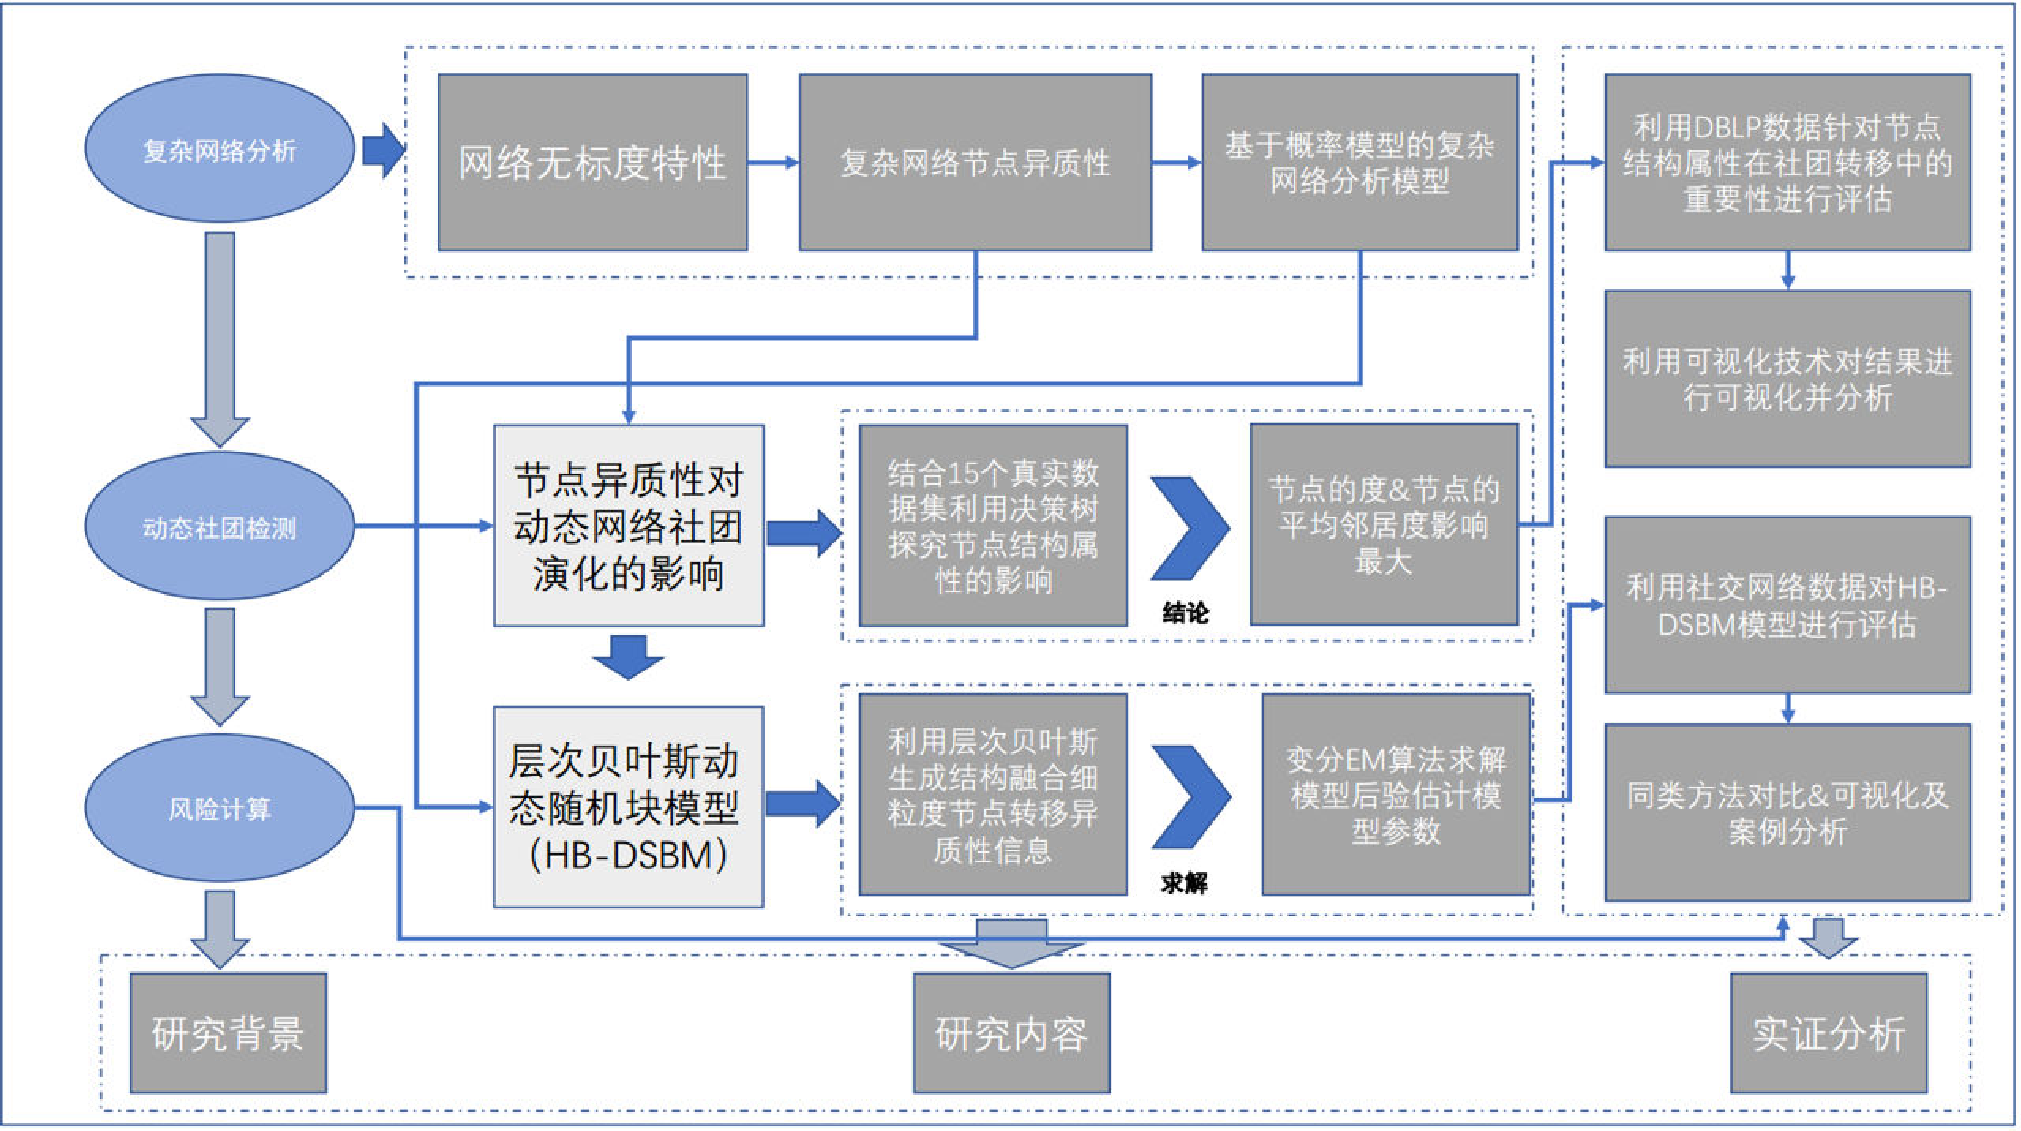
\includegraphics[width = 0.9\textwidth]{./figure/framework1.pdf}
	\caption{研究框架图}
	\label{fig.1}
\end{figure}
以上方法均重点关注动态网络社团检测的精度以及效率,而对于社团演化的关注度并不高。然而社团演化对于动态网络社团检测至关重要,同时社团演化也是一个重要的课题。Yang, Jinfeng~\cite{yang2018structural}等人利用每个社团内的关键节点来匹配相邻社团,进而来把握社团的演化。然而核心节点未必能够代表社团。Gergely Palla~\cite{palla2007quantifying}等人提出社团的出生、消亡、分裂、合并、增长、缩小六种社团行为,被其他研究者广泛借鉴。
社团的演化本质上是由节点之间的连边变化驱动的,因此社团的演化行为与社团内部节点的社团转移之间的关系对于社团演化来说至关重要,然而据我们所知目前还没有对这种关系深入的探究。同时,社团的演化行为也是由社团内的节点的变化而驱动的,目前也没有相关的文献进行详细探究。因此,如图\ref{fig.1}所示,以上两个问题就是本课题将要探究的目标,即探究节点异质性对动态网络社团演化的影响以及利用细粒度演化参数构建动态社团检测模型。
\subsection{城市风险计算现状}
城市风险包含的范围非常广,包括自然灾害城市风险(如地震与台风等)、公共事件类城市风险(如踩踏事件与群体恐慌等)、社会安全城市风险(如核泄漏、恐怖袭击、抢劫枪杀等)、公共卫生安全城市风险(如非典、禽流感与艾滋病等)等。因此对于城市风险来说其风险源广,风险数据量大,其综合识别与整体的管控与治理非常困难。然而针对不同的城市风险需求进行有针对化的计算与治理则难度相对较小,同时其某些特定风险计算需求与网络中的相关算法非常契合,例如网络算法中的关键节点识别就可以用来识别城市风险中的风险点,而风险事件识别则对应了动态网络社团检测。例如社团检测算法可以高效的检测出城市中的不同粒度的团体,再结合社团演化分析就可以检测出不同的事件,通过有效地设置损失函数,就可以对事件风险进行打分并排序,确定不同事件的风险大小。


城市风险计算涉及的数据范围非常广,如城市风险计算包括人类行动轨迹、车辆轨迹、人类电子足迹、社交网络数据、转账数据、城市OD流数据等等,均来自于风险监测模块的多元数据收集。收集后的数据维度广,数据量大,并不能直接进行风险计算,因而需要对数据进行融合,即信息融合。通过多维信息的多层级融合,将数据建模成复杂网络形式数据,进行风险计算。根据不同的风险需求,风险计算可以灵活选择不同的网络算法,如风险因素识别可以利用复杂网络中的关键节点识别算法进行提取,而风险事件则可以利用动态社团检测算法进行计算。

\subsection{主要创新点}

本文的主要创新点包括以下三个方面:

\begin{enumerate}
	\item 发现了动态网络中对节点社团转移影响最大的两个结构属性;
	\item 构建了节点粒度级别演化参数的动态网络社团检测生成模型并为模型求解提出了有效的变分近似算法;
	\item 成功探索了复杂网络社团检测与风险计算的紧密关联并进行了验证。
\end{enumerate}

三个创新点具有紧密的内在关联性,本文通过十五个真实世界复杂网络数据集探索了动态网络中节点的社团转移与节点及社团的结构属性之间的关系,发现了影响节点社团转移的两个结构属性:节点的度以及节点的平均邻居度。这两个结构属性均为节点粒度的结构属性,而社团的属性在节点的社团转移中起到的作用不大,说明节点粒度的社团转移参数在模型中是有必要的。受上述的启发,本文提出了节点粒度的动态网络社团检测模型,并利用变分推断近似求解,使模型适用于真实世界复杂网络。而城市风险计算在城市管理中至关重要,而传统的机器学习算法无法处理具有复杂关联的城市多元数据。依赖于复杂网络及复杂网络社团检测算法,对于城市多元关联性数据,本文提出的算法可以有效的进行处理,同时基于本文算法的处理结果,利用城市风险计算的相关算法可以有效的计算不同事件的风险程度,为城市风险计算与复杂网络社团检测搭建了桥梁。


\section{章节安排}


根据本文的研究框架,文章的章节结构安排如下:

第一章,绪论,介绍复杂网络分析中,社团检测在风险计算中的重要作用以及风险计算的相关流程,研究背景及意义、研究内容框架、主要创新点等。

第二章,相关研究,介绍动态网络社团检测以及风险计算的相关研究,同时介绍本文的统一符号表示等。

第三章,节点结构属性对社团演化影响因素的探究,本文会在真实的网络数据中具体探究动态网络社团检测中,节点的哪些结构属性对社团演化影响较大。

第四章,融合节点级别社团转移参数的动态网络生成模型,本文将会针对经典的动态网络社团检测概率模型-----动态随机块模型,融合更细粒度的演化参数,利用层次贝叶斯生成结构构建对社团演化掌握更准确的新模型:层次贝叶斯动态随机块模型,并在接下来介绍针对层次贝叶斯动态随机块模型的变分推断近似解法。

第五章,案例分析,本章会利用手机信令数据结合动态复杂网络社团检测算法以及风险计算的相关理论知识及算法进行实际的风险计算,验证复杂网络在风险计算中的重要作用。

第六章,总结与展望,本章将总结本课题的工作,并对未来工作进行说明与展望。


\clearpage{\pagestyle{empty}\cleardoublepage} % 去除空白页的页眉页脚(每章从奇数页开始,因此有空白页)
% !Mode:: "TeX:UTF-8"

\chapter{相关研究}
第一章简单介绍了复杂网络社团检测的研究现状,包括静态网络社团检测、动态网络社团检测以及动态网络社团演化的研究现状,并简单说明了以上研究的区别以及关联。同时第一章还介绍了城市风险计算的研究现状,以及社团检测在城市风险计算中的重要作用。本章则从具体的方法论角度介绍动态网络社团检测以及社团演化的研究现状与趋势,包括增量聚类、进化聚类和基于模型的聚类方法。为了验证动态社团检测方法的有效性,本章进一步介绍了相关的社团检测评价指标,包含归一化互信息、均方误差和模块度的定义。接着,本章进一步详细介绍城市风险计算的相关研究以及动态社团检测在风险计算中的作用。
\section{动态网络社团检测}

动态网络社团检测本质上包含了静态复杂网络的社团检测(第一个网络快照上)、动态网络社团检测和社团演化分析三个子问题。对于第一个问题可以借用静态网络社团检测的方法完成,而第二个问题则是目前研究者关注的重点,同时第三个问题--社团演化分析则有助于理解社团的演化模式和动态复杂网络的变化规律。如图\ref{fig.3}所示,图中左右两张图是论文引用数据(DBLP数据)在相邻两个时间快照上的社团可视化图,左侧为前一个时间快照,右侧为后一个时间快照,而不同的颜色代表论文所属的研究领域不同,可以看到,下一时刻的社团结构与上一时刻的社团结构变化很大,只有同时融合社团演化规律与动态社团检测方法才能有效的针对动态复杂网络数据进行高精度的社团检测。
\begin{figure}[!htbp]
	\setlength{\abovecaptionskip}{0pt} 
	\setlength{\belowcaptionskip}{10pt} 
	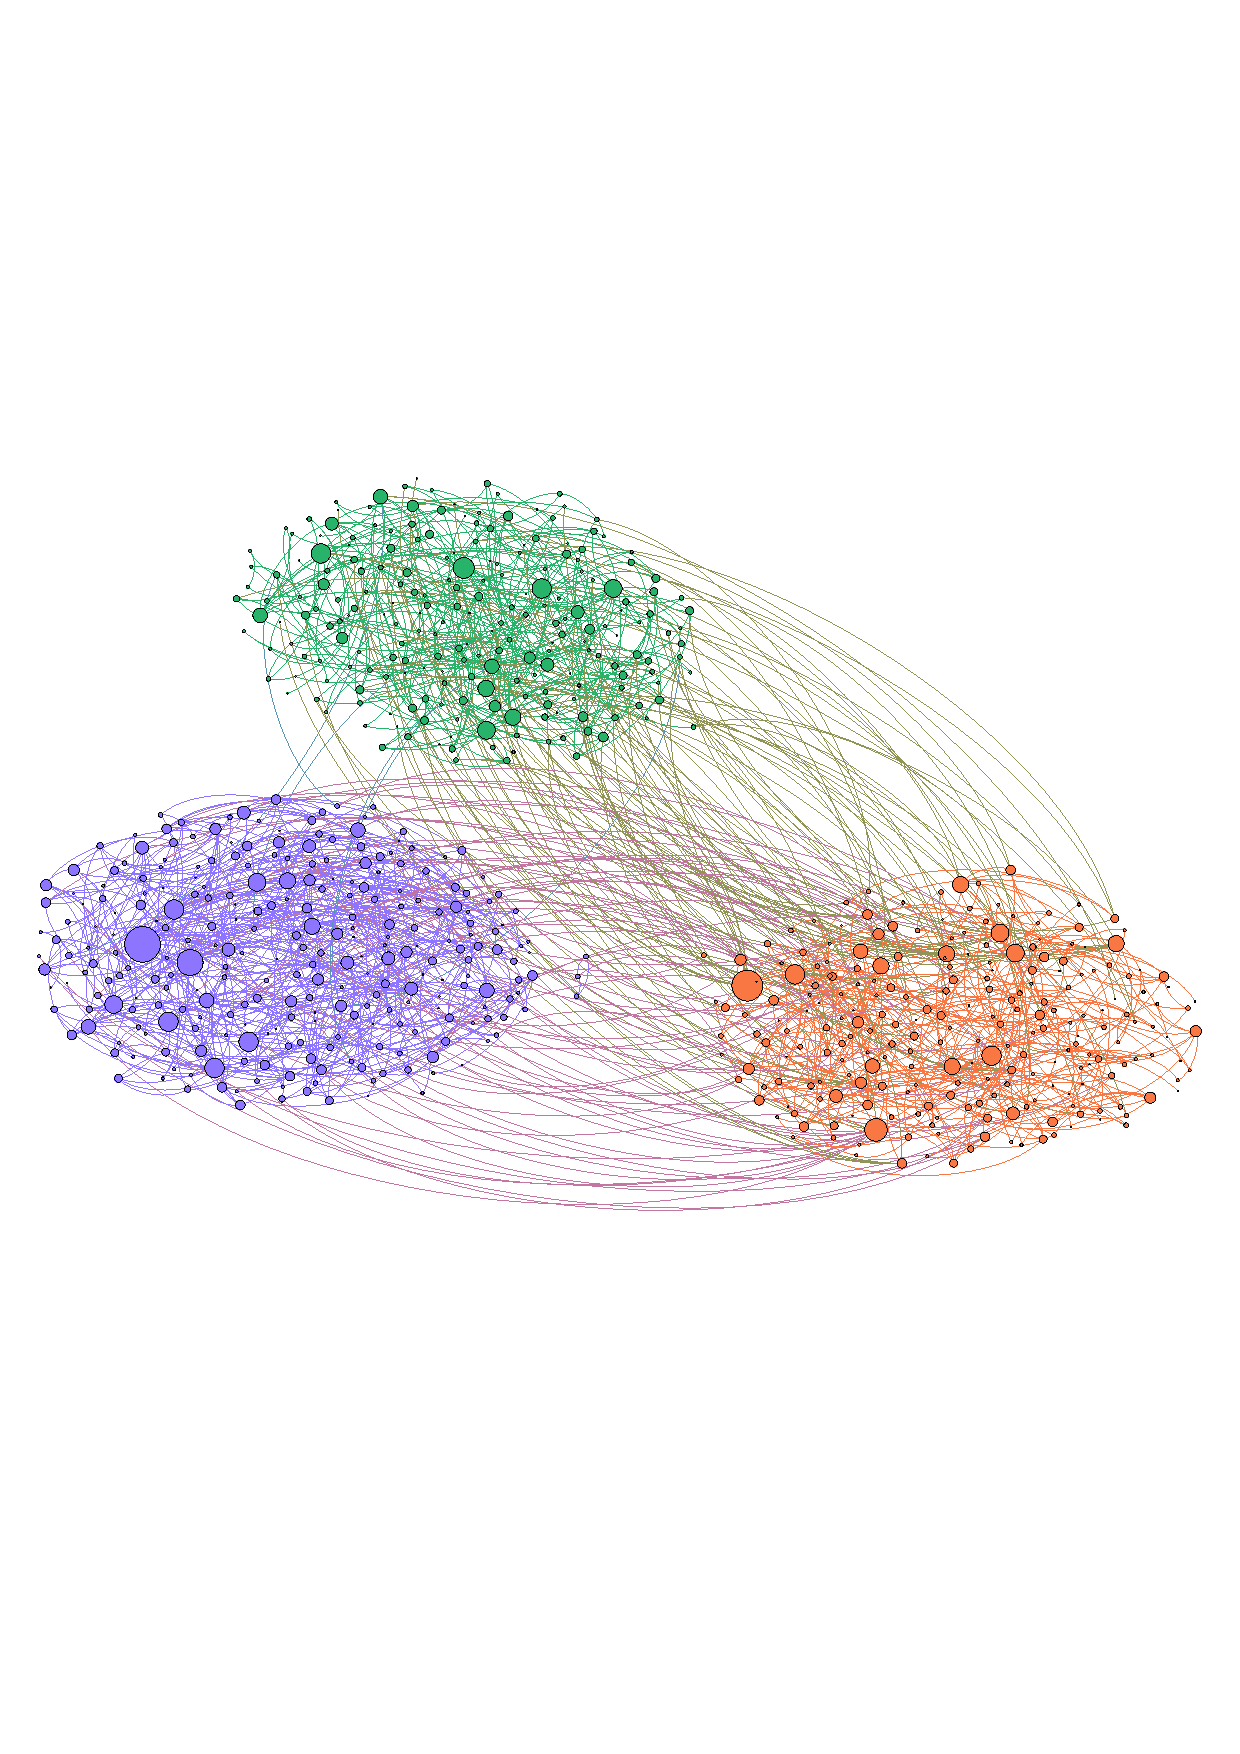
\includegraphics[width=.48\textwidth]{./figure/community1.pdf}
	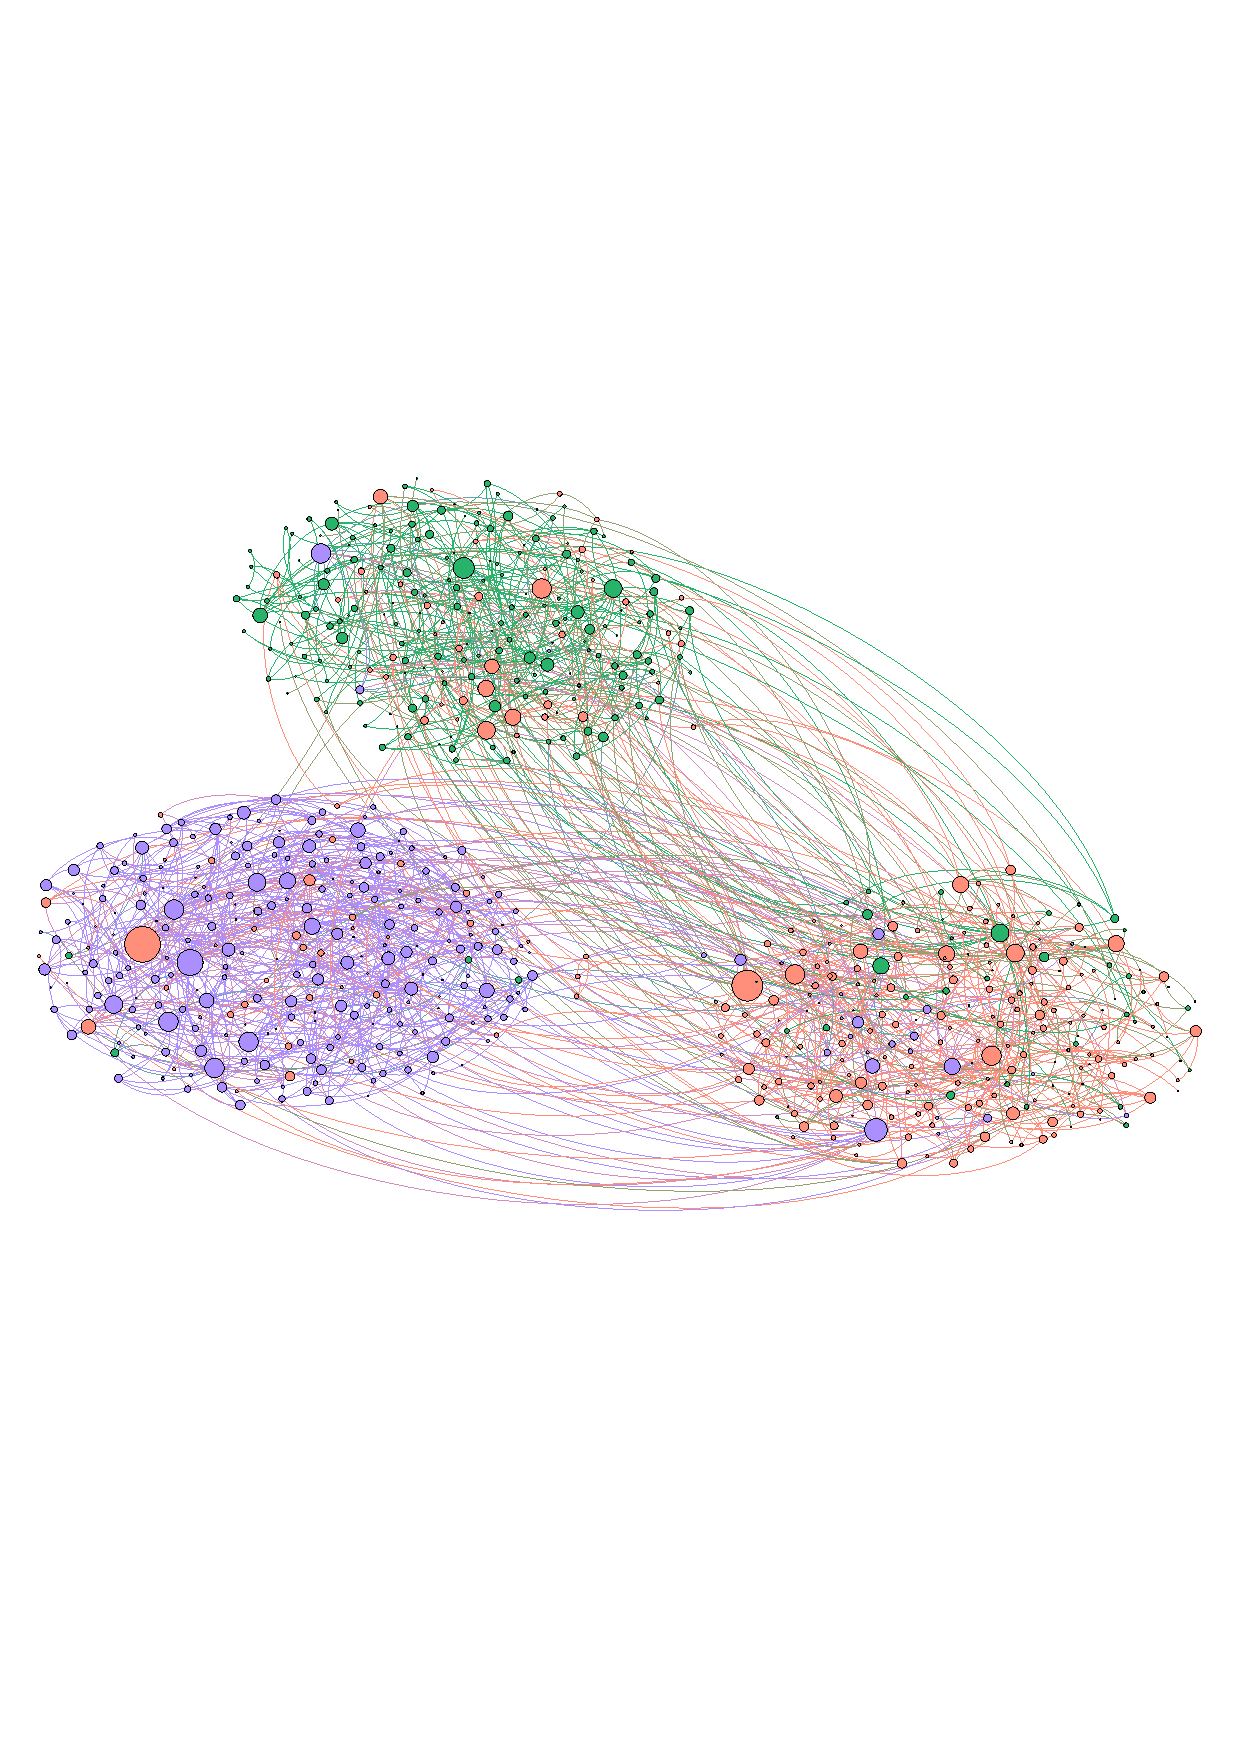
\includegraphics[width=.48\textwidth]{./figure/community2.pdf}
	\caption{论文引用数据(DBLP)的社团及社团演化示意图}
	\label{fig.3}
\end{figure}

目前动态网络社团检测的主流方法将侧重点放在了第二个问题上,根据目前主流的动态复杂网络社团检测方法的本质不同,本文将这些主流方法做出了分类,如表\ref{tab.2.1}所示,增量聚类方法根据不同相邻快照之间的节点和边的变化定义不同的目标函数,增量更新社团信息;进化聚类方法结合了当前网络快照之前的一个或几个快照的信息,来进行当前网络快照的社团检测;而生成模型方法则针对网络以及社团的生成机制进行建模并进行推断,并将动态网络的社团检测问题转化为模型的参数估计问题,从而进行社团检测。
\begin{table}[!htbp]
	\centering
	\caption{主流动态社团检测方法}
	\begin{tabular}[width=\textwidth]{lp{3cm}p{2.5cm}p{2.5cm}p{2cm}}
		\hline
		动态社团检测&核心思想&方法优势&方法不足&代表性工作\\
		\hline  %在第一行和第二行之间绘制横线
		增量聚类方法&将动态网络快照之间社团的变化转化为节点和边的变化,通过定义不同目标函数,增量更新节点的社团归属&复杂度低、对于局部结构变化较多的网络处理更加精准&过于依赖模型定义的目标函数,对网络中的噪声敏感&GraphScope~\cite{sun2007graphscope} GraphTinker~\cite{jaiyeoba2019graphtinker} TILES~\cite{rossetti2017tiles} 模块度优化~\cite{lyf2015} \\
		进化聚类方法&融合动态网络当前快照之前的一个或几个快照社团结构信息,保持社团关系变化的平滑性&融合了历史快照信息,社团检测结果较好&进行大量的网络信息重复计算,复杂度较高&Genlouvain~\cite{jutla2011generalized} PisCES~\cite{liu2018global} DYNMOGA~\cite{folino2014evolutionary} 进化谱聚类~\cite{huang2019community}\\
		生成模型方法&基于隐马尔科夫模型假设,利用生成模型对动态网络进行建模,将社团检测问题转化为参数估计问题&具有严格的理论解释和意义、模型可用于多种网络分析任务&模型优化较困难,同时概率模型的参数较多,参数域较大,因此复杂度较高&动态隐空间模型~\cite{sewell2017latent,yang2015a},动态随机块模型~\cite{yang2011detecting,pensky2017spectral,wu2019dynamic}\\
		\hline % 在表格最下方绘制横线
		
		\label{tab.2.1}
	\end{tabular}
	
\end{table}

\subsection{增量聚类方法}
增量聚类的主要思想是,首先,在动态网络的第一个快照上执行静态社团检测算法,然后根据网络在接下来的快照中的节点和边的变化调整节点的社团归属。Sun等人提出了GraphScope~\cite{sun2007graphscope}方法,GraphScope避免了额外的参数设置(如社团个数、节点的社团转移阈值等),利用信息论的最短描述长度来判别节点的社团变化,并通过处理流数据提升了算法的计算效率。GraphScope在二分网络上具有很好的效果。GraphTinker~\cite{jaiyeoba2019graphtinker}通过定义多种不同的哈希策略来提升传统增量聚类的运行效率和精度,较传统增量聚类运行效率有两倍以上的提升。TILES~\cite{rossetti2017tiles}利用标签传播来刻画节点在网络中的局部变化,以此来减少计算节点在不同时间片上的社团变化的复杂度,同时,标签传播方法还一定程度上避免了单纯的定义目标函数造成的错误累积问题,于此同时,TILES还通过定义不同的触发机制来判定社团的分裂以及合并等演化行为。而IDCD~\cite{lyf2015}方法则通过对第一个时间片的网络对边进行重要性排序,然后通过最大化模块度来检测第一个时间片的社团结构,随后根据后续时间片节点的Jaccard相似度对相应节点的边进行排序,随后按照重要性降序对边关联的节点进行社团划分,该算法的复杂度很低,但是在真实网络中效果并不好。

总的来说,增量聚类在动态网络社团检测中具有效率高,易由静态网络社团检测方法进行迁移等优点,但是其缺点也很明显,由于增量聚类依赖于定义的目标函数,因此存在错误率累积的问题,这使得该方法对数据的噪声过于敏感,因此大部分增量聚类的方法在真实数据中的效果都不是很好。

\subsection{进化聚类方法}

进化聚类方法的主要思想是,该类方法认为动态网络在相邻的时间片时不会发生突变的,因此动态网络的社团结构在相邻时间片或某足够小的时间窗口内的变动是平滑的,所以这类方法在检测某网络快照的社团时,会融合当前快照之前的社团信息,以此来保持节点社团变化的平滑性。Chakrabarti等人首次提出了进化聚类\cite{chakrabarti2006evolutionary},并定义了进化聚类的框架。其本质可表示为
\begin{equation}
	\begin{split}
		Loss = \alpha \times HL + (1-\alpha) \times PL
	\end{split}
\end{equation}
其中Loss表示进化聚类目标函数的整体损失,HC表示当前快照的社团检测结果与上一快照社团检测结果变化的损失,而PC则为当前网络快照的社团检测目标函数的损失,$\alpha$则代表平衡因子,用来控制历史快照对当前快照社团检测的影响力。

 Genlouvain~\cite{jutla2011generalized}继承自Mucha等人2010年在Science上提出的广义网络质量函数框架~\cite{mucha2010community},模型通过定义动态网络连续时间片的\textit{null model},从而得到了动态网络的模块度的定义$Q_{multislice}$。利用动态网络模块度优化,进而得到动态网络的社团划分结果。Folino等人则提出了DYNMOGA~\cite{folino2014evolutionary},DYNMOGA方法基于多目标优化将进化聚类目标函数的两个部分建模为多目标优化问题,并利用遗传算法对模型进行求解。Liu等人提出了PisCES~\cite{liu2018global}方法,通过特征向量平滑的方法约束动态网络的社团在相邻时间片变动尽可能变小,同时考虑到同社团内节点的异质性,PisCES融入了节点的度使其更能适应真实世界网络。 Huang等人~\cite{huang2019community}则结合了Fiedler特征向量与一定时间窗口的正则化拉普拉斯矩阵,进一步用谱聚类的方法进行社团检测。
 
 总的来说,通过融合了动态网络历史社团信息,进化聚类的效果要优于增量聚类方法,但是由于进行社团计算时需要引入更多信息,其复杂度要高于增量聚类。同时,由于参数$\alpha$的存在,使得模型需要进行额外的调参,不利于实际使用。
%\begin{equation}
%\begin{split}
%& Q_{multislice} = \frac{1}{2\mu}\sum_{ijsr}[(A_{ijs}-\gamma_s \frac{k_{is}k_{js}}{2m_s}\delta_{sr})+\delta_{ij}C_{jsr}]\delta(g_{is},g_{jr}) \\
%\end{split}
%\end{equation}

\subsection{生成模型方法}

生成模型方法认为节点的社团转移服从隐马尔科夫假设,通过对复杂网络进行概率建模,来构建网络的生成机制,进而将动态网络的社团检测转化为概率模型的参数估计问题。这部分的方法分类两个大类,分别为隐空间模型和动态随机块模型。

\textbf{隐空间模型}认为,节点的社团划分可以通过将节点在网络中的结构映射到多维的欧式空间中使其变得可分,进而通过利用传统机器学习聚类或者分类算法可以对其进行划分。Daniel K. Sewell等人~\cite{sewell2017latent}提出了动态网络有向和无向两个隐空间模型,定义了不同的距离函数,利用MCMC采样对模型进行求解。Yang等人\cite{yang2015a}针对非负矩阵分解以及谱聚类等利用矩阵计算的隐空间模型提出了一个新的惩罚项,用以提升这些方法通过半监督学习对不完全数据进行社团检测的效果。

而\textbf{动态随机块模型}则继承自随机块模型,有Yang等人\cite{yang2011detecting}于$2011$年通过加入社团转移矩阵A将随机块模型扩展到了动态网络。动态随机块模型认为动态网络中的任意两个节点有边的概率只与节点所在的社团有关,一个节点在一个时间片只能属于一个社团,同时在同一个社团的两个节点在社团检测与社团演化行为上是完全等价的。基于以上假设,得以构建动态随机块模型DSBM,模型通过吉布斯采样结合模拟退火算法进行参数估计,进而得到每个节点在每个时间片上的社团归属。DSBM在进行参数估计之前需要提前指定社团个数,这在真实数据进行社团检测时是不现实的,因此Tang等人~\cite{tang2014detecting}提出了DBTDP,不用社团转移矩阵决定节点的社团转移,而是通过狄利克雷过程刻画节点的转移,利用中国餐馆过程对模型进行模型选择,从而实现了模型自动确定社团个数。动态随机块模型的另一个假设,即一个节点在一个时间片只能属于一个社团,在某些真实场景中也是不合理的,比如大学里每个人可以参与多个社团,或者一个人可以有多种兴趣等等。针对这种场景,Xu\cite{xu2013dynamic}等人扩展了著名的混合随机块模型MMSB,构建了动态混合随机块模型DMMSB。而Yu\cite{yu2018detecting}等人提出了融合节点变化倾向的动态度修正随机块模型,解决了动态随机块模型第三个假设的缺陷,即同一个社团内的节点在社团转移中是完全等价的,模型融入了节点的度来修正不同节点之间连边的异质性;而对于同一社团内节点异质性的把握,Xunxun Wu等人\cite{wu2019dynamic}提出了DPSBM,给出了不同的思路,通过在动态随机块模型中引入了度衰减参数,并假设该参数随时间变化服从半正太分布而演化,从而刻画出了动态网络中节点度分布服从power law的无标度属性。

总体来说,生成模型的方法通过对网络的生成机制进行建模,从而探究了网络生成的本质,使其根据有可解释性,然而由于是对整个网络进行建模,因此其参数数量较增量聚类和进化聚类更大,其参数的解空间更大。同时由于其模型结构的复杂性,使得对模型的参数估计多为MCMC对解空间进行全局搜索,因此其效果更好的同时,复杂度也比前两种方法更高。

\section{动态网络社团演化}

针对动态网络社团检测的第三个子问题,即动态网络相邻时间快照的节点社团演化分析,也一直有人在关注,但是目前还处于起步阶段,对节点随着时间发生社团转移的本质依然没有统一的定论。Dakiche等人\cite{dakiche2019tracking}就社团演化追踪进行了总结,本小结参考他们的总结并结合实际将动态网络社团演化划分为独立社团演化、非独立社团演化以及同步社团演化进行三大类,如表~\ref{tab.2.2}所示。可以看到表中的部分方法与上一小节有重叠,因为动态网络社团检测的不同方法侧重点不同,但是对社团检测以及社团演化一定都有涉及。

\begin{table}[htbp]
	\centering
	\caption{动态社团演化方法}
	\begin{tabular}[width=\textwidth]{lp{3cm}p{2.5cm}p{2.5cm}p{2cm}}
		\hline
		动态社团演化&核心思想&方法优势&方法不足&代表性工作\\
		\hline  %在第一行和第二行之间绘制横线
		独立社团演化&即熟知的两步法,在每个时间片单独进行社团检测,随后对相邻时间片进行社团匹配&容易从发展较好的静态网络社团检测算法进行扩展,可以独立定义社团演化机制&过于依赖定义的社团演化机制,对社团检测效果没有帮助& 基于社团演化事件的方法~\cite{asur2009an,palla2007quantifying,brodka2013ged} \\
		非独立社团演化&假设社团在相邻时间片上不会发生突变,在进行社团检测时定义相应的惩罚项约束社团的演化&社团演化由惩罚函数进行控制,可以加强社团检测效果&进行大量的网络信息重复计算,复杂度较高,无法处理网络的突变&进化聚类~\cite{jutla2011generalized,liu2018global,folino2014evolutionary}  关键节点追踪~\cite{gao2016evolutionary}\\
		同步社团演化&基于隐马尔科夫模型假设,利用生成模型对动态网络进行建模,同时建模社团结构以及其演化规则&具有严格的理论解释和意义、模型可用于多种网络分析任务,社团检测结果与社团演化相互增强&模型优化较困难,同时概率模型的参数较多,参数域较大,因此复杂度较高&DSBM~\cite{yang2011detecting} 涂色优化法~\cite{tantipathananandh2011finding} DPSBM~\cite{wu2019dynamic}\\
		\hline % 在表格最下方绘制横线
		
		\label{tab.2.2}
	\end{tabular}
	
\end{table}

\subsection{独立社团演化}

独立社团演化将动态网络的社团检测与社团演化分别进行独立的计算,在每个时间片执行静态社团检测方法,随后在相邻时间片处理两个社团集合的匹配问题。社团匹配的方法大多基于相似性指标进行匹配,同时这类方法还定义了社团的演化事件,通过确定社团的演化事件来追踪社团的演化。Asur等人\cite{asur2009an}定义了社团的五个可能事件,分别为社团的消失、形成、延续、分裂和合并。而Palla等人\cite{palla2007quantifying}则提出了社团的六种演化事件,分别为增长、缩小、出生、消亡、分裂和合并。在此之后,Brodka等人\cite{brodka2013ged}则融合了前两种事件,提出了社团增长、缩小、延续、出生、消亡、分裂和合并七种演化事件。对于这些事件的检测,以上三组团队均选择在相邻两个时间片进行检测,而Tajeuna等人~\cite{tajeuna2015tracking}则选择在整个动态网络上进行社团演化事件检测。

同时对于相邻时间片的社团匹配,也有不同的社团相似性指标,如Greene等人\cite{greene2010tracking}利用了Jaccard系数计算相邻时间片社团的相似性;而Brodka等人\cite{brodka2013ged}则提出了inclusion度量来计算相邻时间片的社团匹配度;于此同时,Tajeuna等人~\cite{tajeuna2015tracking}定义了名为互转换指标的另一种相似性度量。

独立社团演化可以自由定义社团演化追踪的方法方式,对社团演化事件的追踪也更加的细致。但是社团演化行为是建立在每个事件片上社团检测足够准确的基础上的,割裂了社团演化和社团检测,这类方法的动态社团检测结果往往在真实数据集中表现不好,因为真实世界的动态网络往往具有较高的噪声,同时这类方法也考虑不到社团演化对每个时间片社团的影响。

\subsection{非独立社团演化}
非独立社团演化将社团演化融入到相邻的时间片,以此来增强社团检测效果。这部分包括上一小节介绍的进化聚类的相关方法,如Genlouvain~\cite{jutla2011generalized}PisCES~\cite{liu2018global}DYNMOGA~\cite{folino2014evolutionary}等。同时,非独立社团演化还包括了通过追踪关键节点的方法来追踪社团演化,如Gao等人~\cite{gao2016evolutionary}定义了每个社团的领导节点和跟随者节点,并假设每个社团的演化行为是由领导节点的行为导致的,这使得社团的追踪演化为了对领导节点的追踪。

这类方法在相邻社团融合了社团检测和社团演化,对社团演化的追踪也有一定独到之处,但是这种方法由于其前提假设使得其无法应对网络突变,也并不能很好的把握社团演化的本质。
\subsection{同步社团演化}

同步社团演化通过对网络的建模,同时构建了动态网络社团的产生和社团的演化。如DSBM~\cite{yang2011detecting}通过社团转移矩阵$A$来刻画动态网络中节点的社团转移,通过对$A$的估计,即可得到节点在相邻时间片的演化倾向。然而其社团转移矩阵$A$并不随时间变化,因此并不能刻画节点演化倾向的变化。DPSBM~\cite{wu2019dynamic}则利用其构建的节点度衰减参数$\delta$来修正不同时间片不同节点社团转移的异质性,从而利用$\delta$刻画整个网络节点的社团转移,进而把握住社团的演化。除了以上方法,同步社团演化也存在一些启发式优化方法,如Tantipathananandh等人~\cite{tantipathananandh2011finding}将动态网络社团检测建模为连续的图染色问题,通过求解染色问题来刻画每个时间片的社团以及社团的演化。然而该方法是NP的时间复杂度,虽然作者利用一些启发式方法对求解过程进行了优化,其复杂度依然较高。

同步社团演化结合了社团检测和社团演化,对社团检测与社团演化的效果都比较好,但是由于大部分方法建模的侧重点放在了社团检测,对于社团演化事件以及演化行为的更细节的把控程度以及社团演化的本质探究并不深入。同时概率模型的复杂性使得其求解较困难。


\section{城市风险计算}

针对城市风险的研究由来已久,早在$2007$年,吴竹就在政法学刊上发表了《群体性事件预警指标体系研究》~\cite{wu2007group},文章认为,群体性事件预警是通过对社会系统中的不良因素或者负面因子的检测和评估而形成的,因此吴竹在文章中构建了涉及城市群体性事件预警指标体系,包括了六个子系统下的$67$个具体指标,由于这些指标涉及层面太过广,计算难度很大。而随着互联网的发展,网络空间也成为了城市风险的重要因素之一。王连强~\cite{WangLianqiang2016message}在$2006$年提出了信息安全风险的评估方法框架,框架包括了信息安全风险评估方法ISRAM,定义了信息安全风险评估的计算框架以及平台实现;同时还包括了安全风险评估因素的分类研究等。然而其定义的信息安全风险评估计算涉及的变量及因素较多且框架并没有形成完整的系统,可适用性并不好。同时该框架仅仅涉及信息安全风险,并不与城市风险形成关联。龚俭等人~\cite{gongjian2017network}$2017$在软件学报发表了《网络安全态势感知综述》,该综述中提出了网络安全态势感知框架,该框架的态势察觉-态势理解-态势评估模块不仅在网络安全态势感知中获得大部分人的认同,同时给物理空间安全态势感知也提供了有效的参考。文章也同时提出了利用聚类的方法将相似性的警报进行聚类同一整合,减少系统警报数量。

而随着计算机算力的指数性提升,利用计算机结合有效的算法对城市风险进行计算是目前城市风险计算的显而易见的发展方向。然而由于城市数据的维度广,不同层面的数据之间交互复杂,单纯的机器学习算法由于其对数据单元的i.i.d假设导致其并不能准确的计算城市风险。另一方面,城市风险计算方式通过传统的群体性事件预警或者评估方法需要的资源以及计算量非常大,并不能做到有效且实时。因此通过复杂网络对城市数据进行建模,进而利用复杂网络中的相关算法对城市风险进行计算评估是合理且最行之有效的。

利用复杂网络对城市系统进行建模的研究由来已久,如利用复杂网络分析台风对城市的影响~\cite{chenchangkun2012taifeng}、利用复杂网络对电力系统进行建模并分析其脆弱性~\cite{2014electric}、利用复杂网络建模城市道路网络,并分析其脆弱性~\cite{zhangshude2014}等等。由此可见,复杂网络的脆弱性计算~\cite{gou2016topological}应用到城市系统中,可以在很大程度上发现城市的潜在风险。

\begin{figure}[htbp]
	\centering
	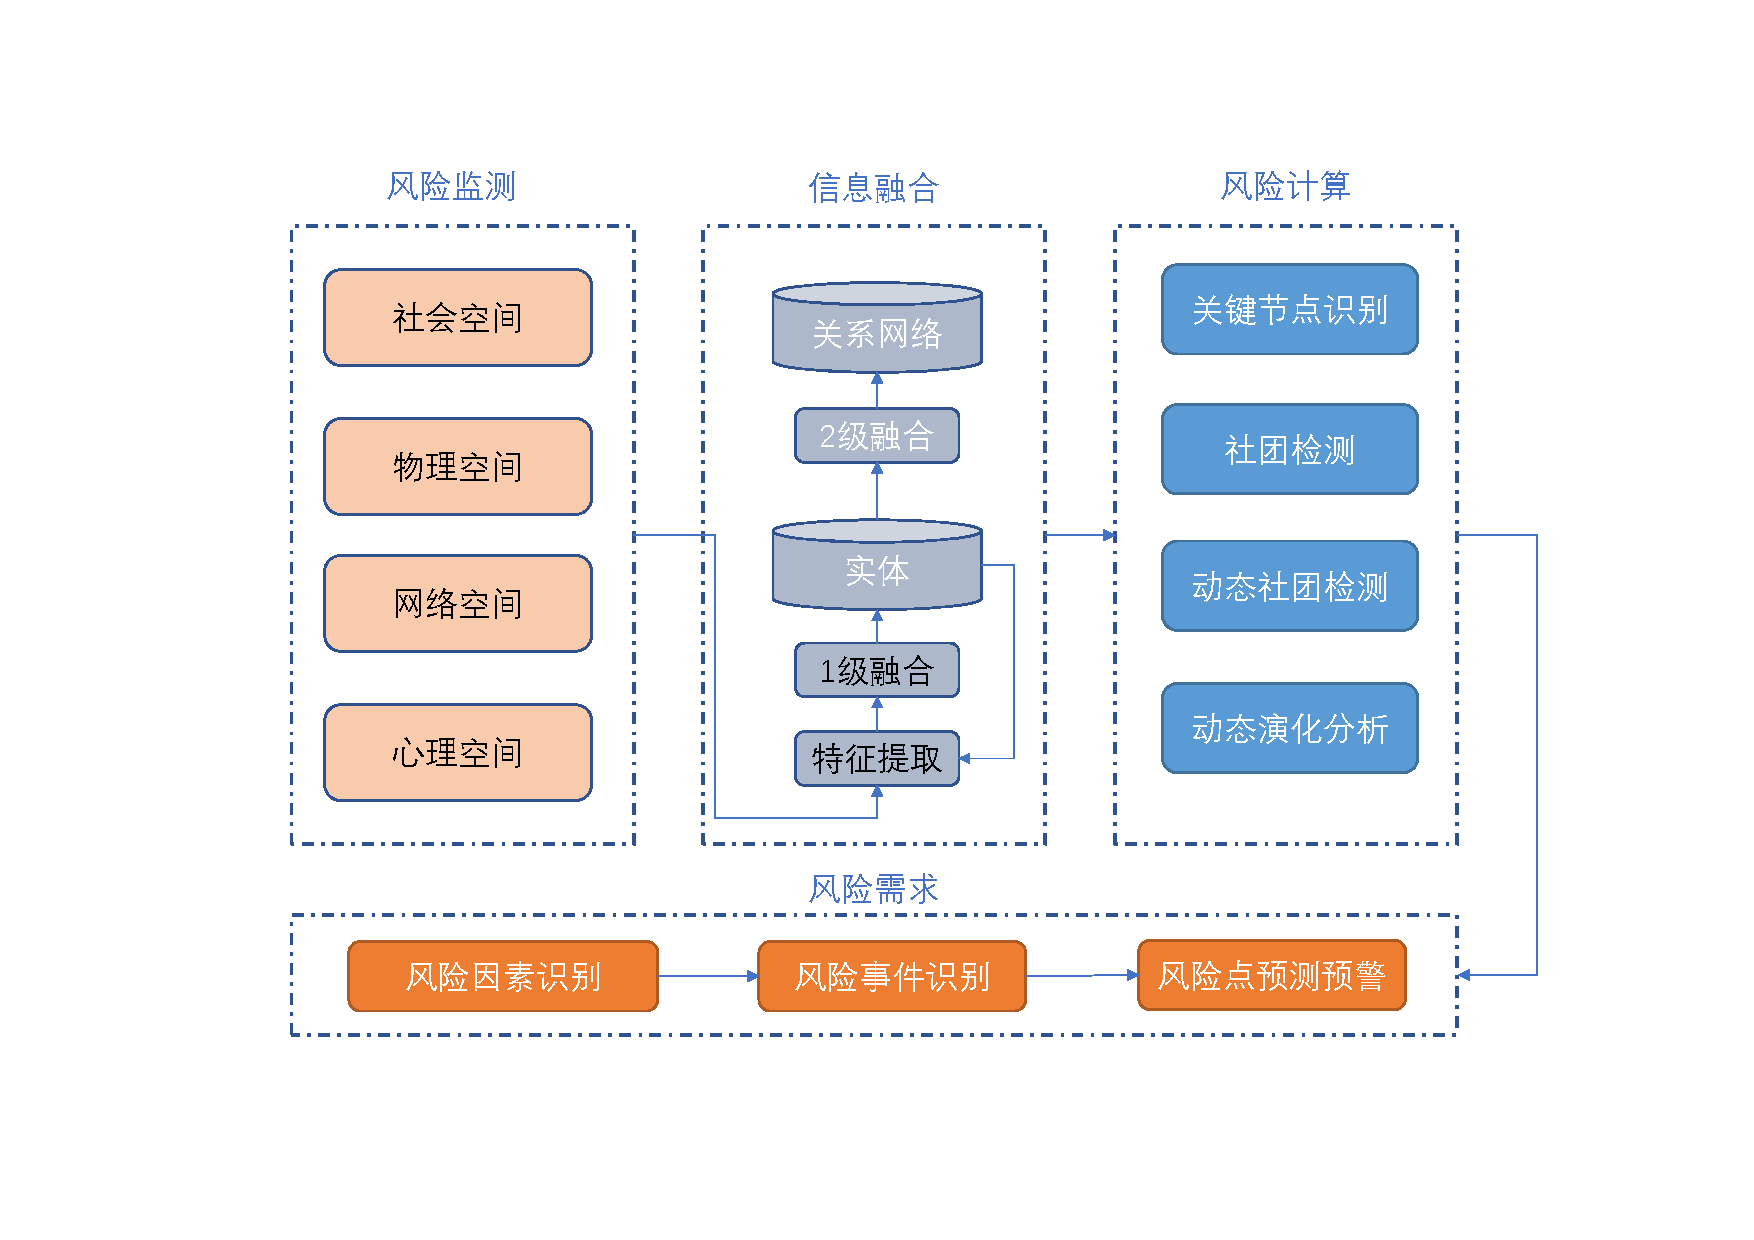
\includegraphics[width = 0.9\textwidth]{./figure/framework2.pdf}
	\caption{风险计算框架图}
	\label{fig.2}
\end{figure}

本文的风险计算研究框架如图\ref{fig.2}所示,通过整合多渠道的城市风险计算流程总结整合而成,首先监测多元空间的数据,并通过信息融合将数据进行预处理、数据对齐等步骤将潜在风险的数据融合处理为实体,进一步经过二级融合将数据构建成复杂网络。根据不同的风险需求,复杂网络算法会在其中起到各不相同的作用。

而动态网络社团检测则能够处理风险事件识别或风险因素识别的风险需求,通过对风险网络中的节点进行动态社团检测,并进一步进行事件提取,随后利用相关的打分算法对不同事件进行打分,随后筛选出潜在的风险事件~\cite{moriano2019community-based}。也可以利用社团演化分析,判断团体的发展走向,结合网络脆弱性指标或者节点重要性指标,综合分析城市中某些团体的潜在威胁。

%\section{符号表示}


\section{本章小结}
本章首先介绍了复杂网络分析的发展历程及其主要任务,随后聚焦于复杂网络分析中的社团检测的相关研究。接着针对动态网络社团检测的目前研究现状以及存在的主要问题进行了阐释说明。最后,本章介绍了风险计算的发展现状与城市风险计算和社团检测的紧密联系进行了说明。

\clearpage{\pagestyle{empty}\cleardoublepage}
% !Mode:: "TeX:UTF-8"

\chapter{节点结构属性对社团演化影响因素的探究}
上一章介绍了动态复杂网络社团检测的相关研究以及城市风险计算的最新进展。上一章提到了社团演化对动态复杂网络社团检测的影响非常大,而目前的大部分方法都聚焦于动态复杂网络的每个时间快照上的社团检测效果而或多或少地忽略了社团演化的重要性。更进一步,本文认为节点的结构属性特别是局部结构对节点社团演化的影响是很大的,因为社团的演化行为是由节点的社团转移行为构成的,也就是说,节点的社团转移行为才是社团演化的驱动力量。因此针对节点的结构属性对节点社团转移的影响的探究是必要且重要的。这也是本章的研究重点,即对节点的结构属性对节点社团转移的影响的探究。本章首先介绍对探究节点结构属性对节点社团转移影响的方法,然后介绍使用的真实世界复杂网络数据集,随后介绍经过第一部分介绍的方法结合第二部分真实数据集分析后得到的结论。
\section{探究方法}

\begin{figure}[!htbp]
	\setlength{\abovecaptionskip}{0pt} 
	\setlength{\belowcaptionskip}{10pt} 
	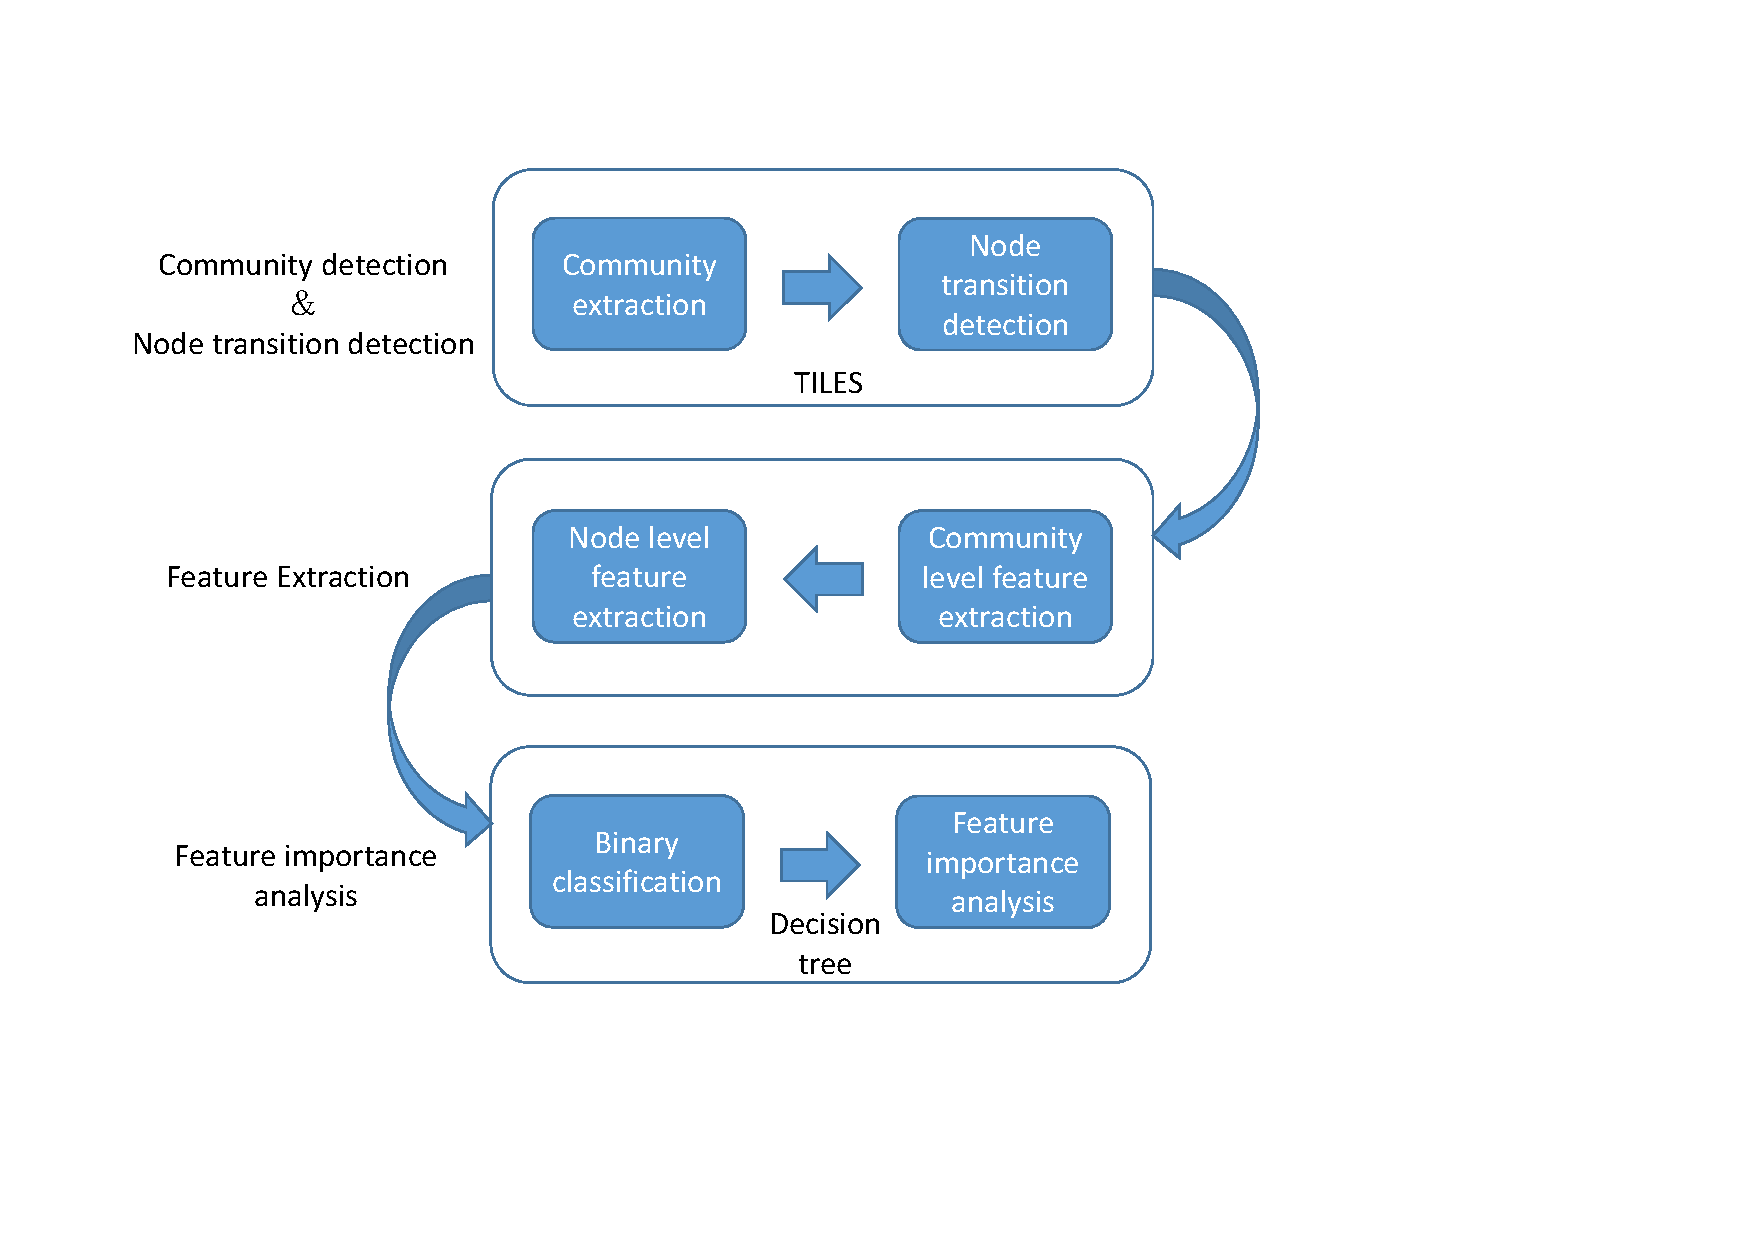
\includegraphics[width=.9\textwidth]{./figure/flowChart3.pdf}
	\caption{探究方法流程图}
	\label{fig.3.1}
\end{figure}

针对节店结构属性对节点社团转移影响的探究方法如图\ref{fig.3.1}所示,该方法共分为三步。
\begin{enumerate}
	\item 社团检测及节点转移检测,首先利用TILES\cite{rossetti2017tiles}对动态网络数据进行社团检测,同时TILES还会将复杂网络三元组数据进行时间片切分,即将$(源点,汇点,时间)$形式的数据处理为传统的动态网络时间片结构$W=\{W^1,W^2,...,W^T\}$,其中$T$为动态网络时间片的个数,而$W^t \in {0,1}^{N \times N}$为$t$时刻的网络邻接矩阵。我们假设所有该框架涉及到的网络均为无权图。随后我们将相邻的网络时间片组成相邻时间片组,并标注其中发生社团转移的节点与未发生社团转移的节点作为分类的节点社团转移标签。
	\item 节点结构特征提取,通过特征工程方法及以往论文的经验\cite{ilhan2016feature},本方法分别提取了五个社团级别结构特征及五个节点级别结构特征共十个结构特征。这些特征分别为:社团节点数、社团边数、社团内部边(即指向社团内部节点的边数)、社团外部边(即从社团内指出的边)、社团活性、社团的传导率、节点度、节点的平均邻居度、节点的接近中心性、节点的介数中心性。其具体描述见表\ref{fig.3.1}。通过相邻时间片组提取节点结构属性的方法见算法\ref{alg1}。
	\item 特征重要性分析,利用决策树对节点社团转移标签进行分类,将第二步提取的节点结构特征作为分类特征进行二分类。分类后,利用MDI计算每个特征在分类任务中的重要性,最终得到不同节点结构特征在节点发生社团转移情景中的重要性。
\end{enumerate}

在该框架的第一步中,框架利用了现有的社团检测框架TILES。TILES是现有的最高水准的基于进化聚类的社团检测算法,其利用标签传播方法检测动态网络中的社团,并在该进程中划分每个动态网络时间片。TILES检测的社团结构是重叠社团,即网络中每个节点可以在一个网络快照中属于多个社团,这给社团转移检测造成了一定难度,即如何界定节点发生社团转移行为。TILES认为重叠社团类似社交网络中的账号可以属于多个圈子,针对这种思路,本框架认为当一个节点在上一时间片转移到本时间片时,其社团归属集中有新社团出现时,则该社团发生了社团转移,因为一个人的精力是有限的,那么当这个人加入了新的社团时,其在原社团中投入的精力就会减小,这也是节点的一种社团转移。

在特征提取步骤中,本文认为节点所属社团也会对节点的转移行为造成影响,例如,在社交网络中,不同的圈子人员流动性是不一样的,或者如不同的组织人员流动性是不一样的。这些组织或群体的特征会影响群体内人员的转移意愿,因此本框架引入了部分社团级别的特征作为节点的结构特征的一部分。

在特征重要性分析中,本文选择了决策树来作为节点转移二分类的分类方法,因为决策树不同于深度神经网络,是白箱算法,因此每个特征的重要性都能通过决策树得到。本文使用Mean Decrease in Impurity(MDI)\cite{menze2009comparison}计算每个特征的重要性,DMI的定义如下:

\begin{equation}
\centering
\Delta i(s,r) = i(r)- p_L i(r_L) - p_R i(r_R)
\end{equation}

其中, $i(r)$ 是一些不纯度度量如gini index. $r$表示某个决策树节点,而$r_L$和$r_R$分别是 $r$的子节点。 $p_L = N_{r_L}/N_r$ 其中$N_r$是通过节点$r$的数据量。类似的$p_R=N_{r_R}/N_r$. 标准化后的$\Delta i(s,r)$可以给每个特征一个重要性度量,同时该计算指标非常高效,因此可以适用于大规模数据。

\begin{table}[!htbp]
	
	\centering
	\caption{notations and definitions}\label{tab.3.1}
	\resizebox{0.99\textwidth}{!}{
		\begin{tabular}{|l|p{70pt}|p{170pt}|l|}
			% \begin{tabular}{|l|l|l|l|}
			\hline
			Symbol&Feature & Description & Definition\\
			\hline
			$f1$&Community node number & Number of nodes within the community $l$ at time $t$. & $n_l^t$\\
			$f2$&Community edge number & Number of edges within the community $l$ at time $t$. & $e_l^t$\\
			$f3$&Intra community edges & Ratio of the total number of edges between the nodes inside the community($e_l^t(in)$) to the number of nodes in the community.& $\frac{e_l^t(in)}{n_l^t}$\\
			$f4$&Inter community edges & Ratio of the total number of edges of nodes connected outside the community($e_l^t(out)$) to the number of nodes in the community. & $\frac{e_l^t(out)}{n_l^t}$\\
			$f5$&Community activity & Ratio of the total number of connections made in the previous snapshot by the nodes of the community($a_l^t$) to the number of nodes in the community. & $\frac{a_l^t}{n_l^t}$\\
			$f6$&Community Conductance & Ratio of the number of edges in the community to the sum of degrees of the nodes in the community. & $\frac{e_l^t}{d_l^t}$\\
			$f7$&Node degree & Sum of links connected to node $i$ at time $t$. & $e_i^t$ \\
			$f8$&Node average neighbor degree & Average degree of node $i$'s neighbors, where $N(i)^t$ are the neighbors of node $i$ at time $t$ and $e_j^t$ is the degree of node $j$ which belongs to $N(i)^t$. & $\frac{1}{|N(i)^t|}\sum_{j\in N(i)^t}e_j^t$ \\
			$f9$&Node closeness centrality & Measuring a node $i$'s average path length to other nodes in community, where $C_{l,-i}^t$ is a set of all nodes in community $l$ except $i$ at time $t$ and $d(i,j)$ is the distance between node i and j.& $\sum_{j\in C_{l,-i}^t}\frac{C_l^t}{d(i,j)}$ \\
			$f10$&Node betweenness centrality & Measuring a node $i$'s importance in its community connectivity, where $\sigma_{jk}$ is the total number of shortest paths from node $j$ to node $k$ and $\sigma_{jk}(i)$ is the number of those paths that pass through $i$ & $\sum_{j,k \in C_{l,-i}^t}\frac{\sigma_{jk}(i)}{\sigma_{jk}}$\\
			\hline
		\end{tabular}
	}
\end{table}


\begin{algorithm}[!htbp]
	\caption{Feature extraction}
	\label{alg1}
	\algorithmicrequire \quad A sequence of undirected graphs $W = {W}^1,..{W}^T$ and the community assignment $\mathcal{C} = \mathcal{C}^1,...\mathcal{C}^T$\\
	\algorithmicensure \quad Nodes feature set $F$ and nodes label set $L$
	\begin{algorithmic}[1]
		\FOR{every graph ${W}^t$ where $t \neq T$}
		\FOR{every community $\mathcal{C}_l^t$ in $\mathcal{C}^t$ }
		\STATE Calculate community level features $F_c$
		\FOR{every node $i$ in community $\mathcal{C}_l^t$}
		\STATE Calculate node level features $F_n$
		\STATE Compose node $i$'s feature sequence $F = F_c + F_n$
		\IF{node $i$ changes its community in ${W}^{t+1}$}
		\STATE node $i$'s label $L_i$ = 1
		\ELSE
		\STATE node $i$'s label $L_i$ = 0
		\ENDIF
		\ENDFOR
		\ENDFOR
		\ENDFOR
	\end{algorithmic}
\end{algorithm}




\section{数据集}

本章所用数据集包括因特网数据、Facebook数据、手机信令数据即Wiki数据等共15个多类型网络公开复杂网络数据集,对于数据集的详细描述见表\ref{tab.3.2}。如图\ref{fig.3.2}所示,所有数据的节点度分布都服从power-law。




\begin{table}[!htbp]
	\centering
	\caption{data sets description}\label{tab.3.2}
	\resizebox{0.99\textwidth}{!}{
		\begin{tabular}{|p{70pt}|p{250pt}|p{40pt}|p{40pt}|}
			\hline
			Name & Description & $|\mathcal{V}|$ & $|\mathcal{E}|$\\
			\hline
			Internet & Internet\cite{mislove-2009-socialnetworksthesis} topology during $04/01/2004 -04/04/2005.$& $33936$ & $104824$\\
			Facebook & Facebook New Orleans networks\cite{viswanath-2009-activity} friends links during $06/08/2008-21/01/2009.$&$62306$& $905565$\\
			bitcoin & Who-trusts-whom network of people who trade using Bitcoin on Bitcoin OTC \cite{kumar2016edge} during $09/11/2010-19/01/2016.$ & $5881$ & $35592$\\
			Friend & Call logs of members of a young-family residential living community adjacent to a major research university in North America\cite{aharony2011social} during $10/07/2010-16/07/2011.$ & $130$ & $60518$\\
			fb-forum & The Facebook-like Forum Network\cite{nr} during $15/05/2004-24/10/2004.$ & $899$ & $33720$\\
			fb-messages & The Facebook-like Social Network\cite{nr} from an online community for students at University of California during $24/03/2004-22/10/2004.$ & $1897$ & $61734$\\
			ia-digg-reply & A reply network of the social news website Digg\cite{nr} during $29/10/2008-13/11/2008.$ & $30397$ & $87627$\\
			ia-facebook-wall-wosn-dir & The Facebook friendship graph\cite{nr} during $15/05/2004-24/10/2004.$ & $44668$ & $876993$\\
			ia-reality-call & The MIT Reality mining a small set of human call logs data\cite{nr} during $24/09/2004-07/01/2005. $& $6810$ & $52050$\\
			ia-slashdot-reply-dir & Reply network of technology website Slashdot\cite{nr} during $01/12/2005-31/08/2006.$ & $51097$ & $140778$\\
			ia-stackexch-user-marks-post & User answering question network of Stack Overflow\cite{nr} during $03/10/2008-25/11/2011.$ & $545196$ & $1302439$\\
			ia-yahoo-messages & The message network in yahoo\cite{nr} with time presented by  link sequences. & $99303$& $3179718$\\
			soc-epinions-trust-dir & Epinion who-trusts-whom network\cite{nr} with time presented by  link sequences. & $131828$ & $841373$\\
			soc-wiki-elec & Wikipedia adminship election data\cite{nr}during $14/09/2004-05/01/2008.$ & $8271$ & $107071$\\
			wiki& The Wikipedia links data \cite{mislove-2009-socialnetworksthesis} during $20/02/2001-06/12/2002.$ & $329623$ &$39953145$\\
			\hline
		\end{tabular}
	}
\end{table}


\begin{figure}[!htbp]
	\setlength{\abovecaptionskip}{0pt} 
	\setlength{\belowcaptionskip}{10pt} 
	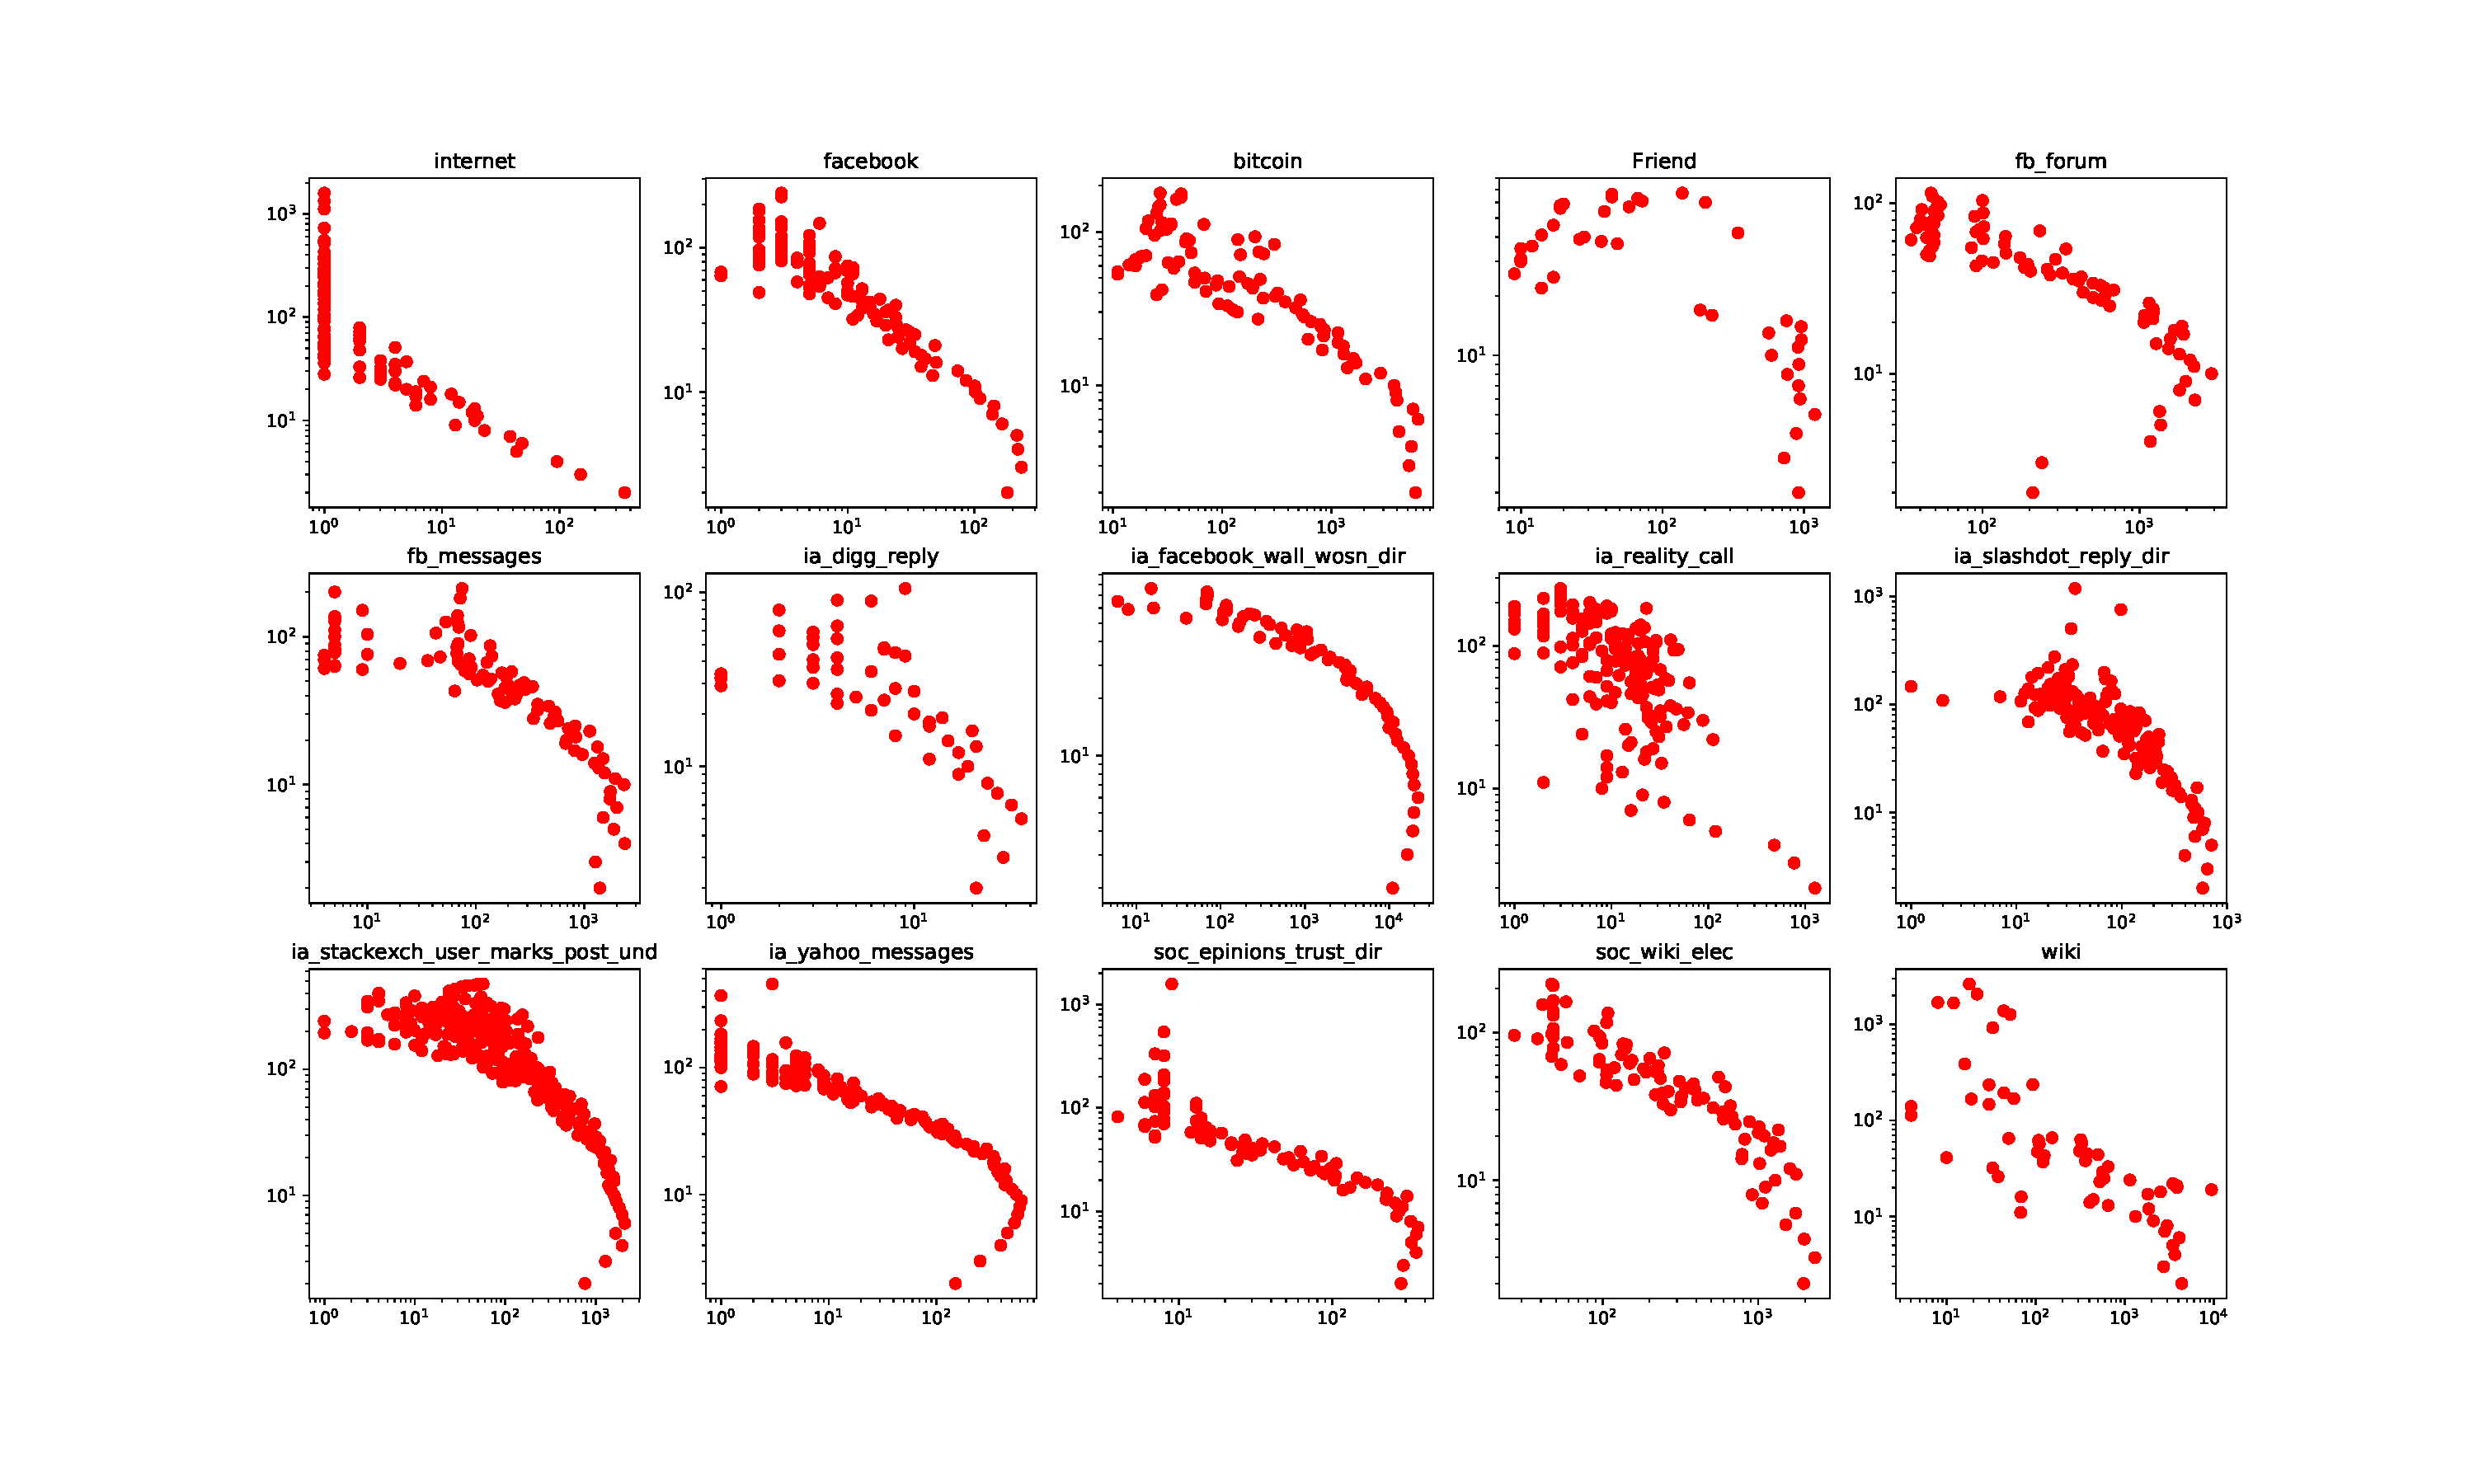
\includegraphics[width=.9\textwidth]{./figure/degrees.pdf}
	\caption{15个真实数据集的度分布可视化}
	\label{fig.3.2}
\end{figure}

\section{实验及验证}

\subsection{实验及结论}

按照上文所述的研究框架处理上述$15$个数据集,并计算其特征重要性。结果如热图\ref{fig.3.3}所示,横坐标表示节点的分类特征,即分类特征;纵坐标分别表示$15$个数据集,颜色代表特征在不同数据集中的分类任务中所占重要性。可以看到$f7$(节点的度)与$f8$(节点的平均邻居度)在所有特征分类中均占很大比重,尤其在$fb-forum$数据中,节点的平均邻居度在分类中所占比重超过了0.5;而$f5$(社团活跃度)在$ia-slashdot-reply-dir$数据中所占比重超过其他数据,该数据为技术网站Slashdot的回复网络,从这一点来看,\textbf{科技类网站的圈子活跃度}是影响其用户更换兴趣圈的主要因素;与此同时,在$internet$网络中,$f9$(节点的接近中心性)对其节点的社团转移影响最大,显而易见,在因特网中,连通性是其最至关重要的指标之一。虽然$f5,f9$均在某些数据集中显示出了对节点社团转移的重要影响力,但是其并不具有普遍性。反观$f7,f8$,其在所有数据集中对节点的社团转移均具有可观的影响力。因此我们得出结论,\textbf{节点的度以及节点的平均邻居度是影响节点发生社团转移的重要的结构特征}。


\begin{figure}[!htbp]
	\setlength{\abovecaptionskip}{0pt} 
	\setlength{\belowcaptionskip}{10pt} 
	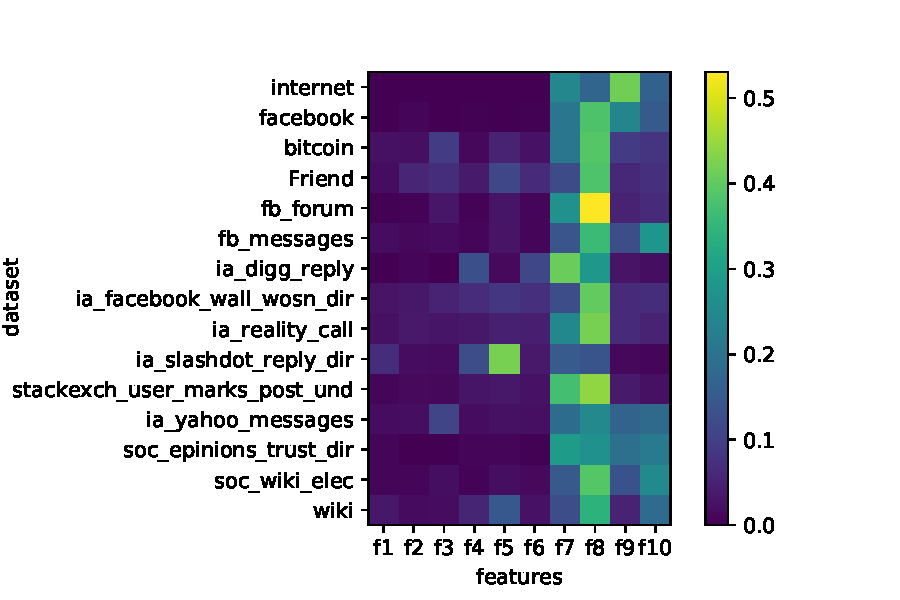
\includegraphics[width=.9\textwidth]{./figure/15cmp.pdf}
	\caption{15个数据集的特征重要性热图}
	\label{fig.3.3}
\end{figure}

为了探究节点的度以及节点的平均邻居度是以何种模式影响节点的社团转移的,本文分别统计了以上两个节点结构属性在$15$个数据集中的分布。如图\ref{fig.3.4}所示,该图展示了节点的度在十五个数据集中的分位图,每个子图中共有两列分位图,分别为发生转移的节点(横坐标为$1$)以及未发生转移的节点(横坐标为$0$)的度的分位统计图。从图中可以看到,在所有$15$个数据集中,发生社团转移的节点的度普遍比未发生转移的节点的度更高,即在一个网络中,节点的度越高,其越有可能转移其所在的社团。这也验证了社团检测中的大量度修正方法~\cite{wilson2016modeling,jin2015modeling}的正确性。而图\ref{fig.3.5}则展示了节点的平均邻居度在十五个数据集中的分位图,每个子图中共有两列分位图,分别为发生转移的节点(横坐标为$1$)以及未发生转移的节点(横坐标为$0$)的平均邻居度的分位统计图。可以看到节点的平均邻居度在不同数据集中的发生转移以及未发生转移节点中的值并不相同,这说明不同的节点平均邻居度确实在影响节点的社团转移行为,然而其模式在所有十五个数据集中并不统一。

\begin{figure}[!htbp]
	\setlength{\abovecaptionskip}{0pt} 
	\setlength{\belowcaptionskip}{10pt} 
	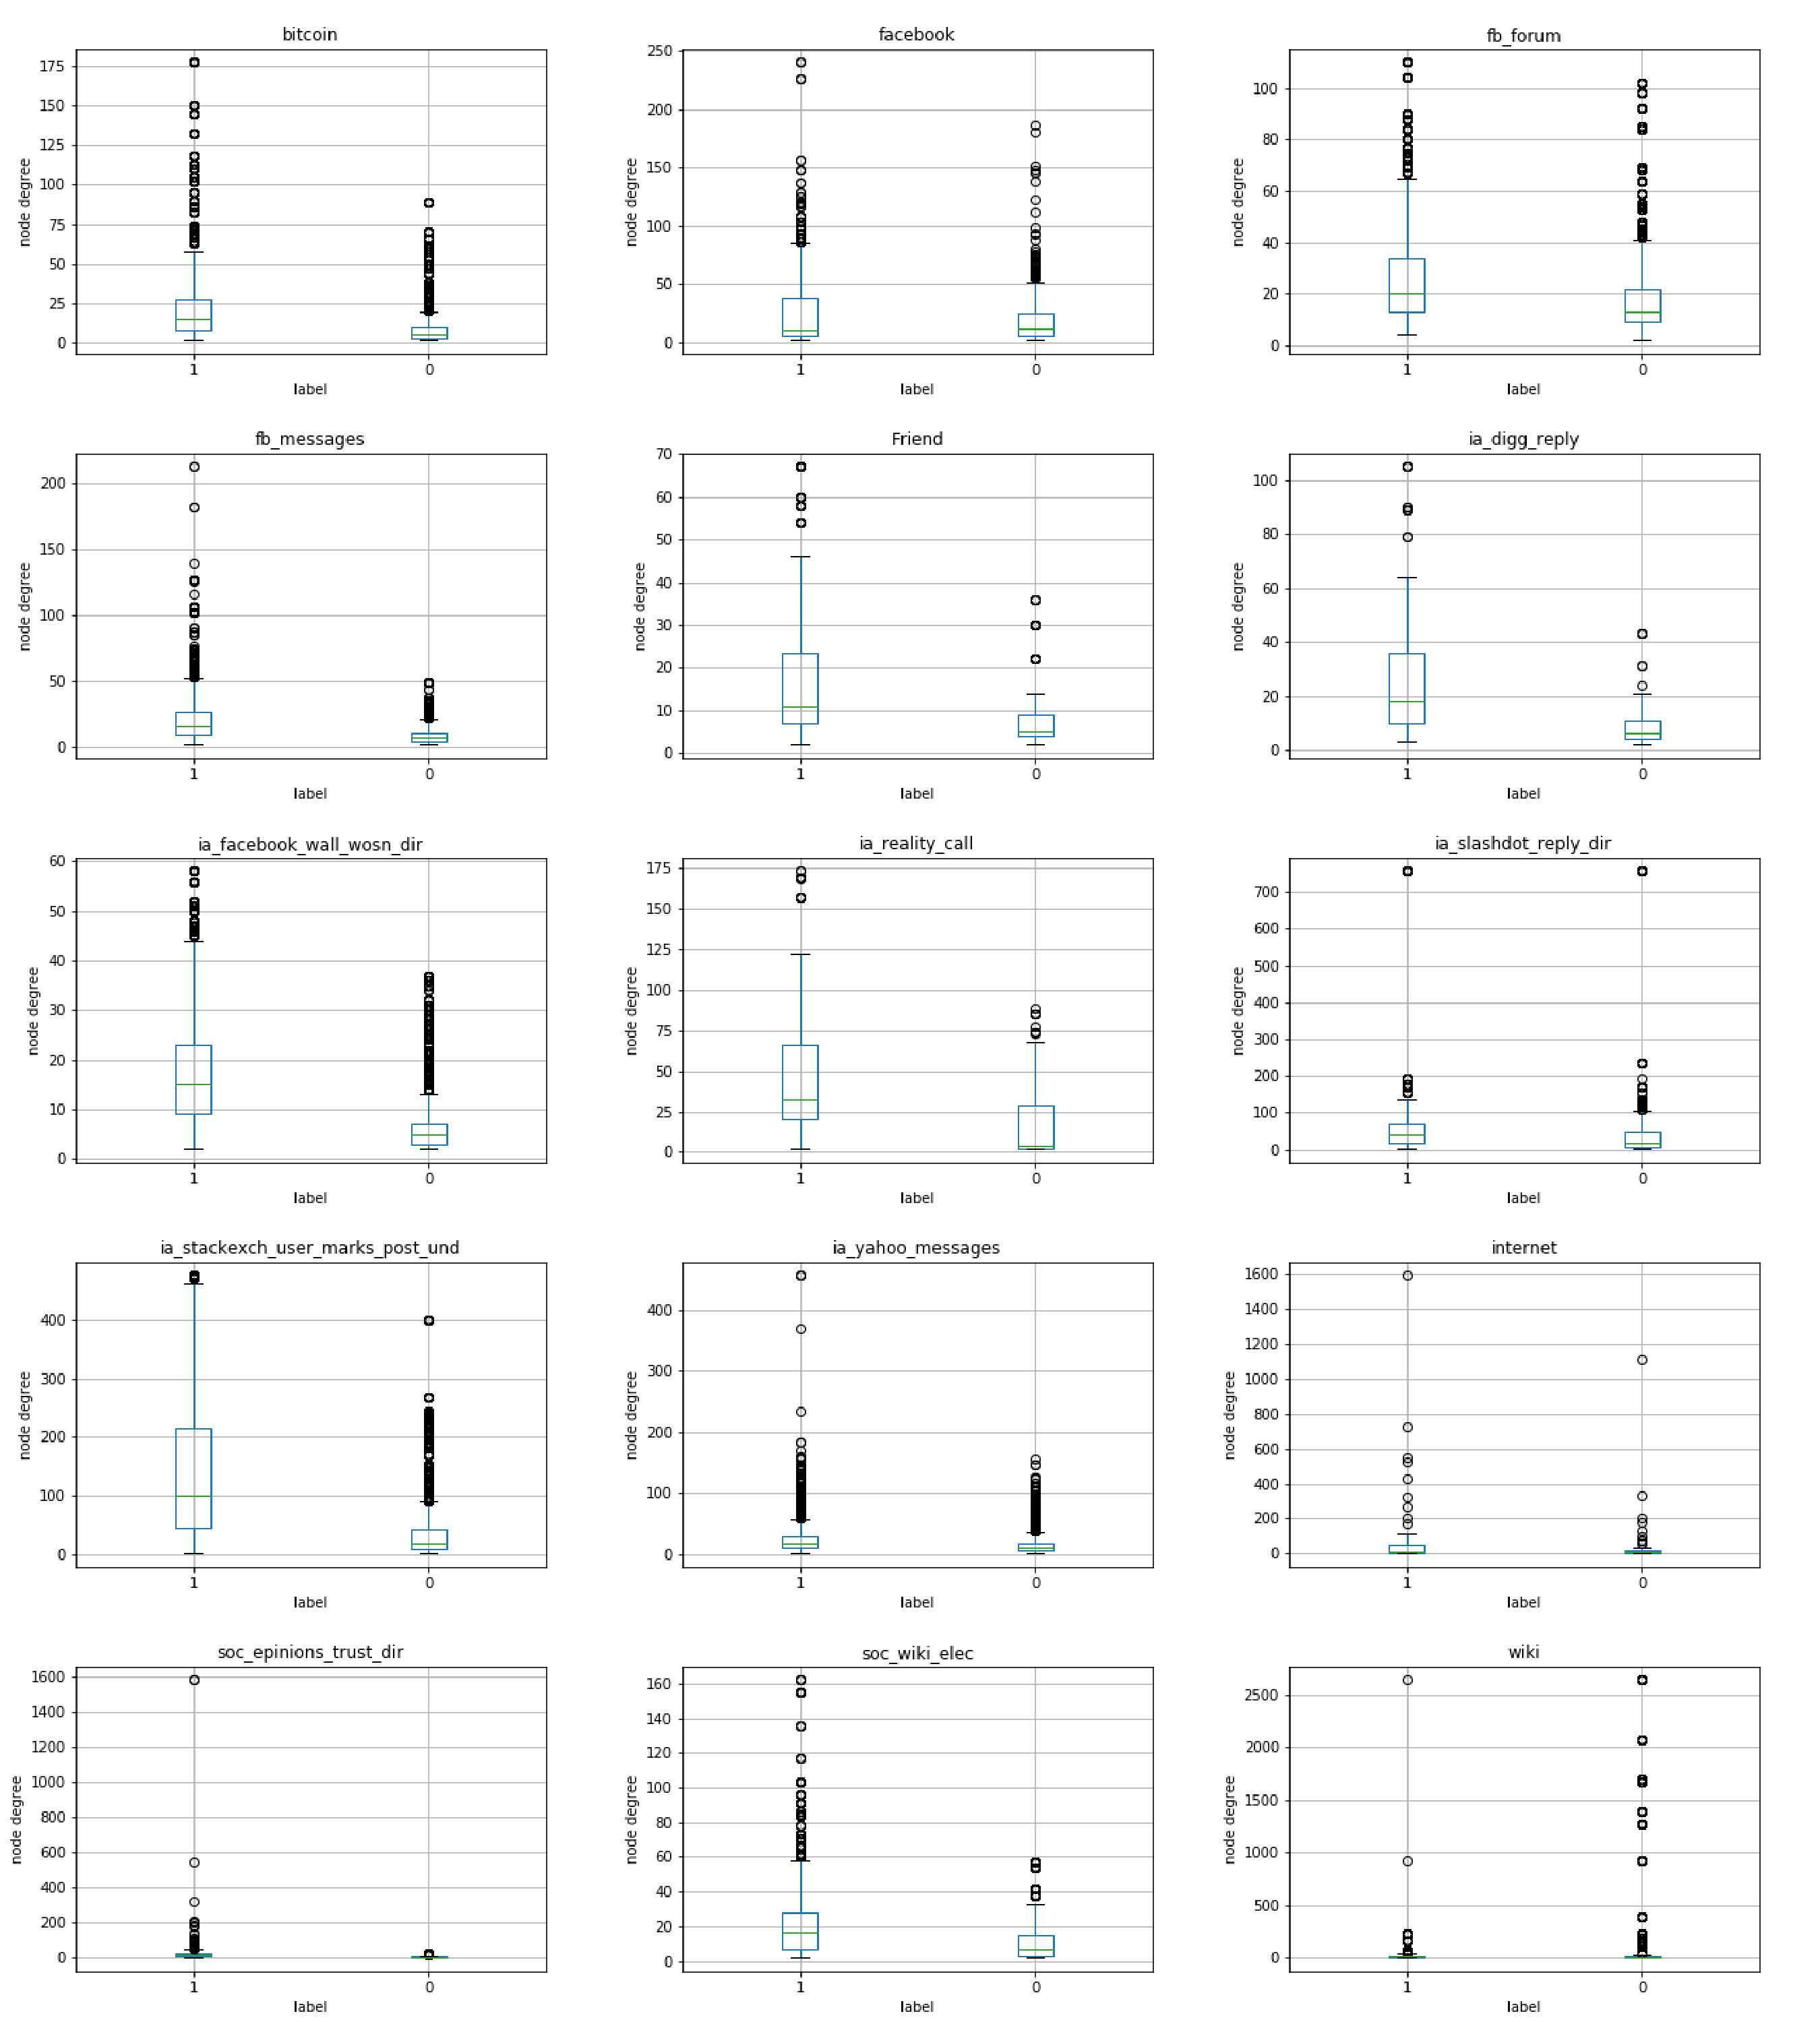
\includegraphics[width=.9\textwidth]{./figure/alldata-DG.pdf}
	\caption{15个数据集的节点度的分位图}
	\label{fig.3.4}
\end{figure}

\begin{figure}[!htbp]
	\setlength{\abovecaptionskip}{0pt} 
	\setlength{\belowcaptionskip}{10pt} 
	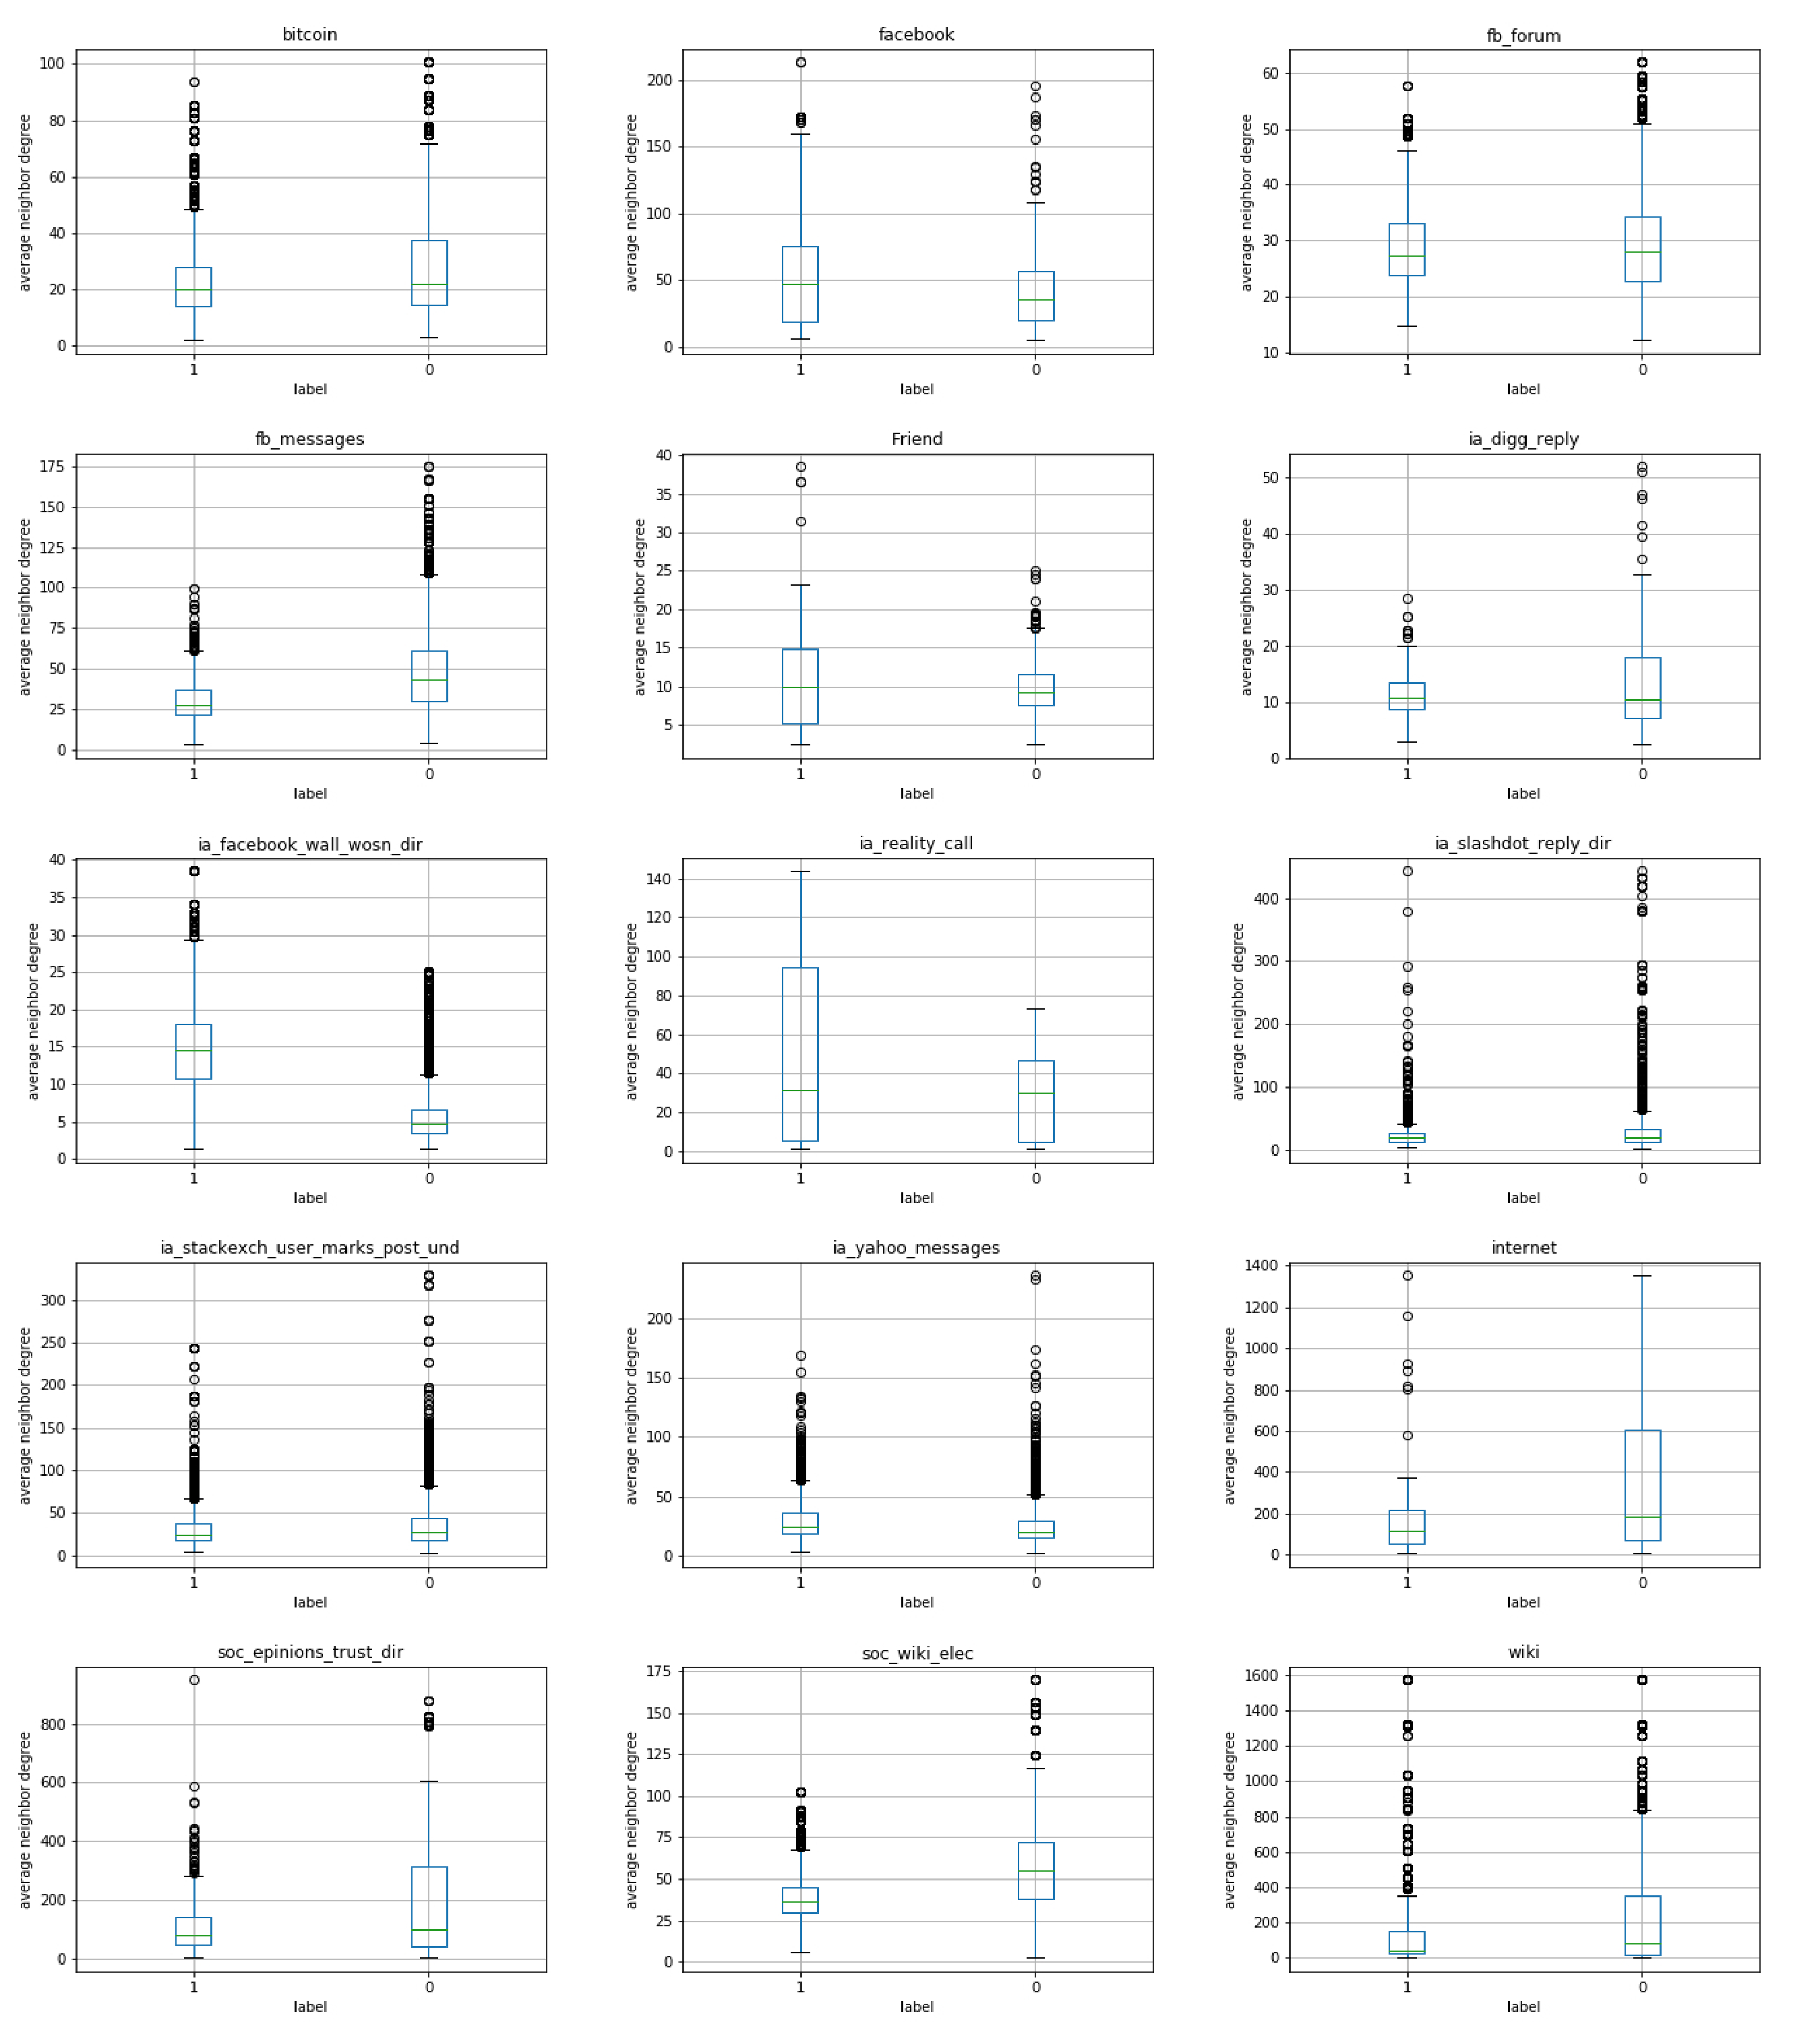
\includegraphics[width=.9\textwidth]{./figure/alldata-aND.pdf}
	\caption{15个数据集的节点的平均邻居度的分位图}
	\label{fig.3.5}
\end{figure}


\subsection{验证}

为了验证结论\textbf{节点的度及节点的平均邻居度影响节点的社团转移},本文在论文引用网络DBLP中支撑结论的案例。如图\ref{fig.3.6}所示,图中节点代表论文作者,而节点大小代表节点的度的大小。不同颜色代表节点所属社团不同,即不同颜色作者的研究兴趣不同,同时节点上的文字代表“平均邻居度-作者名”,例如“4.82-$Shuicheng Yan$”代表作者名为$Shuicheng Yan$的平均邻居度为$4.82$。

其中图\ref{a}\ref{b}展示了平均邻居度给论文作者带来的影响,图\ref{a}与图\ref{b}是相邻时间快照($2005$年和$2006$年)的相同作者的论文发表可视化图。可以看到,$Jun Yan,Zheng Chen$和$Ning Liu$ 都具有较高的平均邻居度$9.33$,受他们共同的具有较高节点度的邻居$Shuicheng Yan$的影响,在$2006$年,他们转移了原有的研究兴趣领域,在\texttt{TKDE}上与$Shuicheng Yan$合作发表了与$Shuicheng Yan$相同研究兴趣的论文\footnote{Yan, Jun, et al. "Effective and efficient dimensionality reduction for large-scale and streaming data preprocessing." IEEE transactions on Knowledge and Data Engineering 18.3 (2006): 320-333.}。

而图\ref{c}\ref{d}则展示了节点度对论文作者带来的影响,图\ref{c}和图\ref{d}也是相邻时间快照($2005$年和$2006$年)相同作者的论文发表可视化图。如图所示,$Marc Pollefey$所属的节点具有较大的直径,即其节点度较大,这代表着他的朋友较多,而由图\ref{c}可以看出,他的绝大部分朋友都与他所在的研究兴趣领域不同。受其朋友影响,他在$2006$年改变了其研究兴趣领域。更详细的说,他与他的合作者$Jan-Michael Frahm$在$2006$年在\texttt{EDGE}共同发表了一篇论文 \footnote{Sinha, Sudipta N., et al. "GPU-based video feature tracking and matching." EDGE, workshop on edge computing using new commodity architectures. Vol. 278. 2006.}。从图中的两个较小的节点$Roland Memisevic$和$Christopher Zech$也能看出平均邻居度的影响,这二人都具有较高的平均邻居度$8.33$,而受到两人共同的朋友$Marc Pollefeys$的影响,他们也在$2006$年改变了研究兴趣领域。

\begin{figure}[!htbp]
	\centering
	\subfigure[]{
	\begin{minipage}[t]{0.48\textwidth}
		\centering
		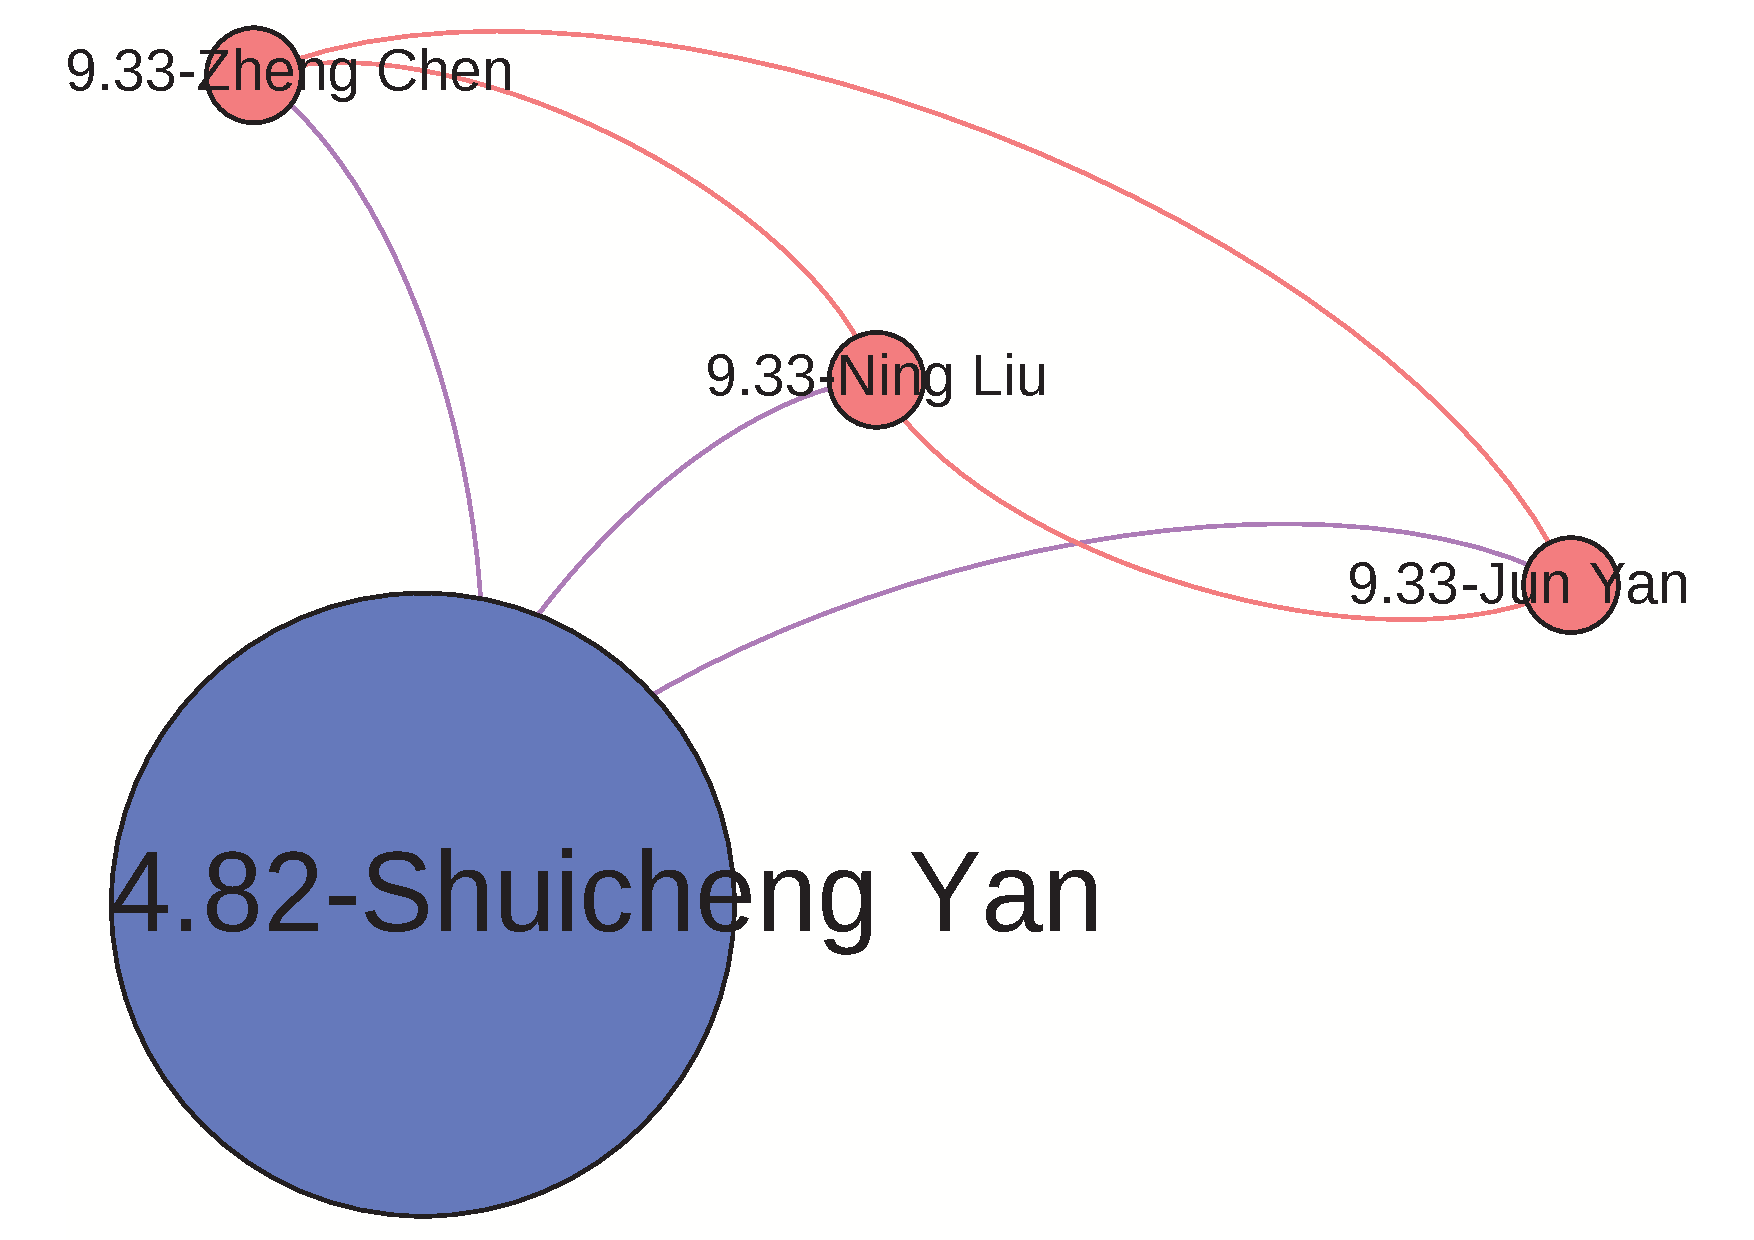
\includegraphics[width=4cm]{./figure/ca0.pdf}
		\label{a}
	\end{minipage}}
	\subfigure[]{
	\begin{minipage}[t]{0.48\textwidth}
		\centering
		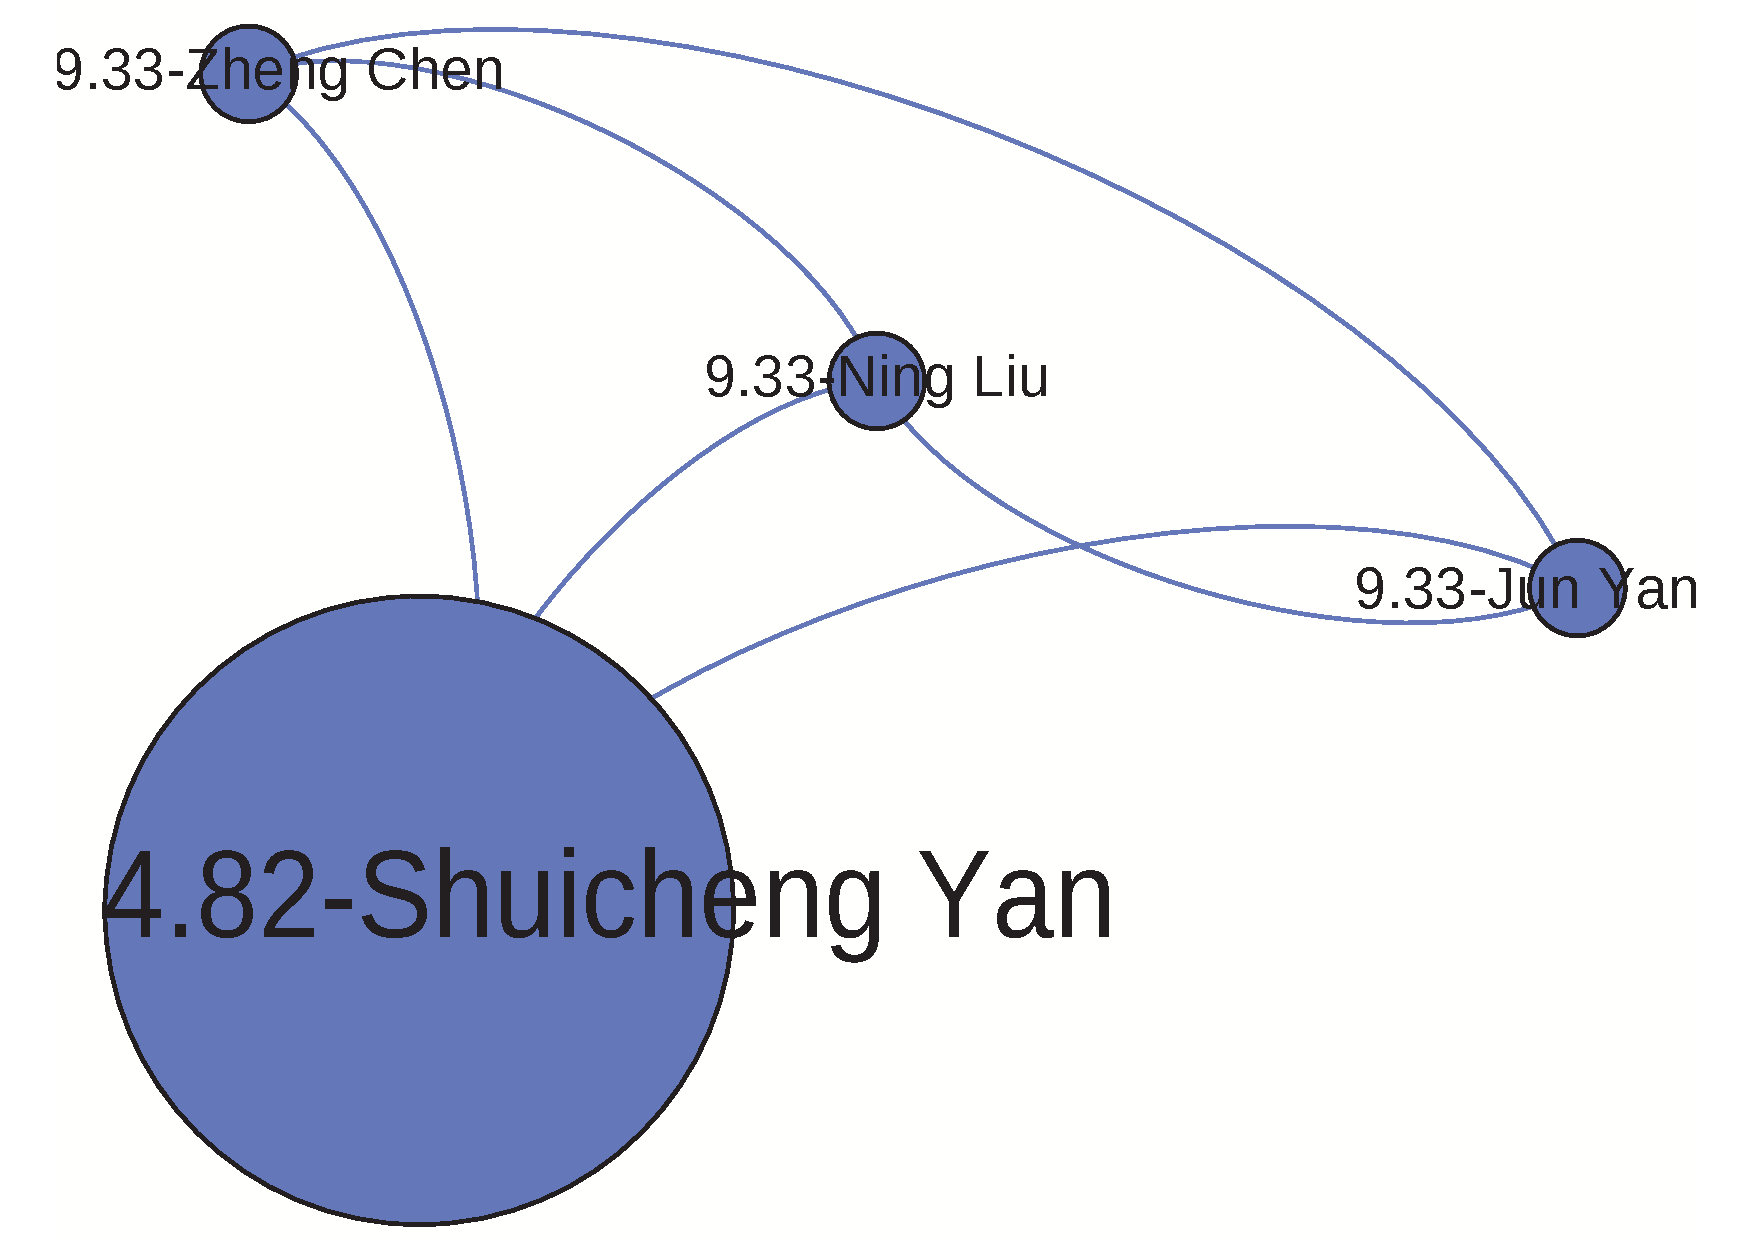
\includegraphics[width=4cm]{./figure/ca1.pdf}
		\label{b}
	\end{minipage}}
	\subfigure[]{
	\begin{minipage}[t]{0.48\textwidth}
		\centering
		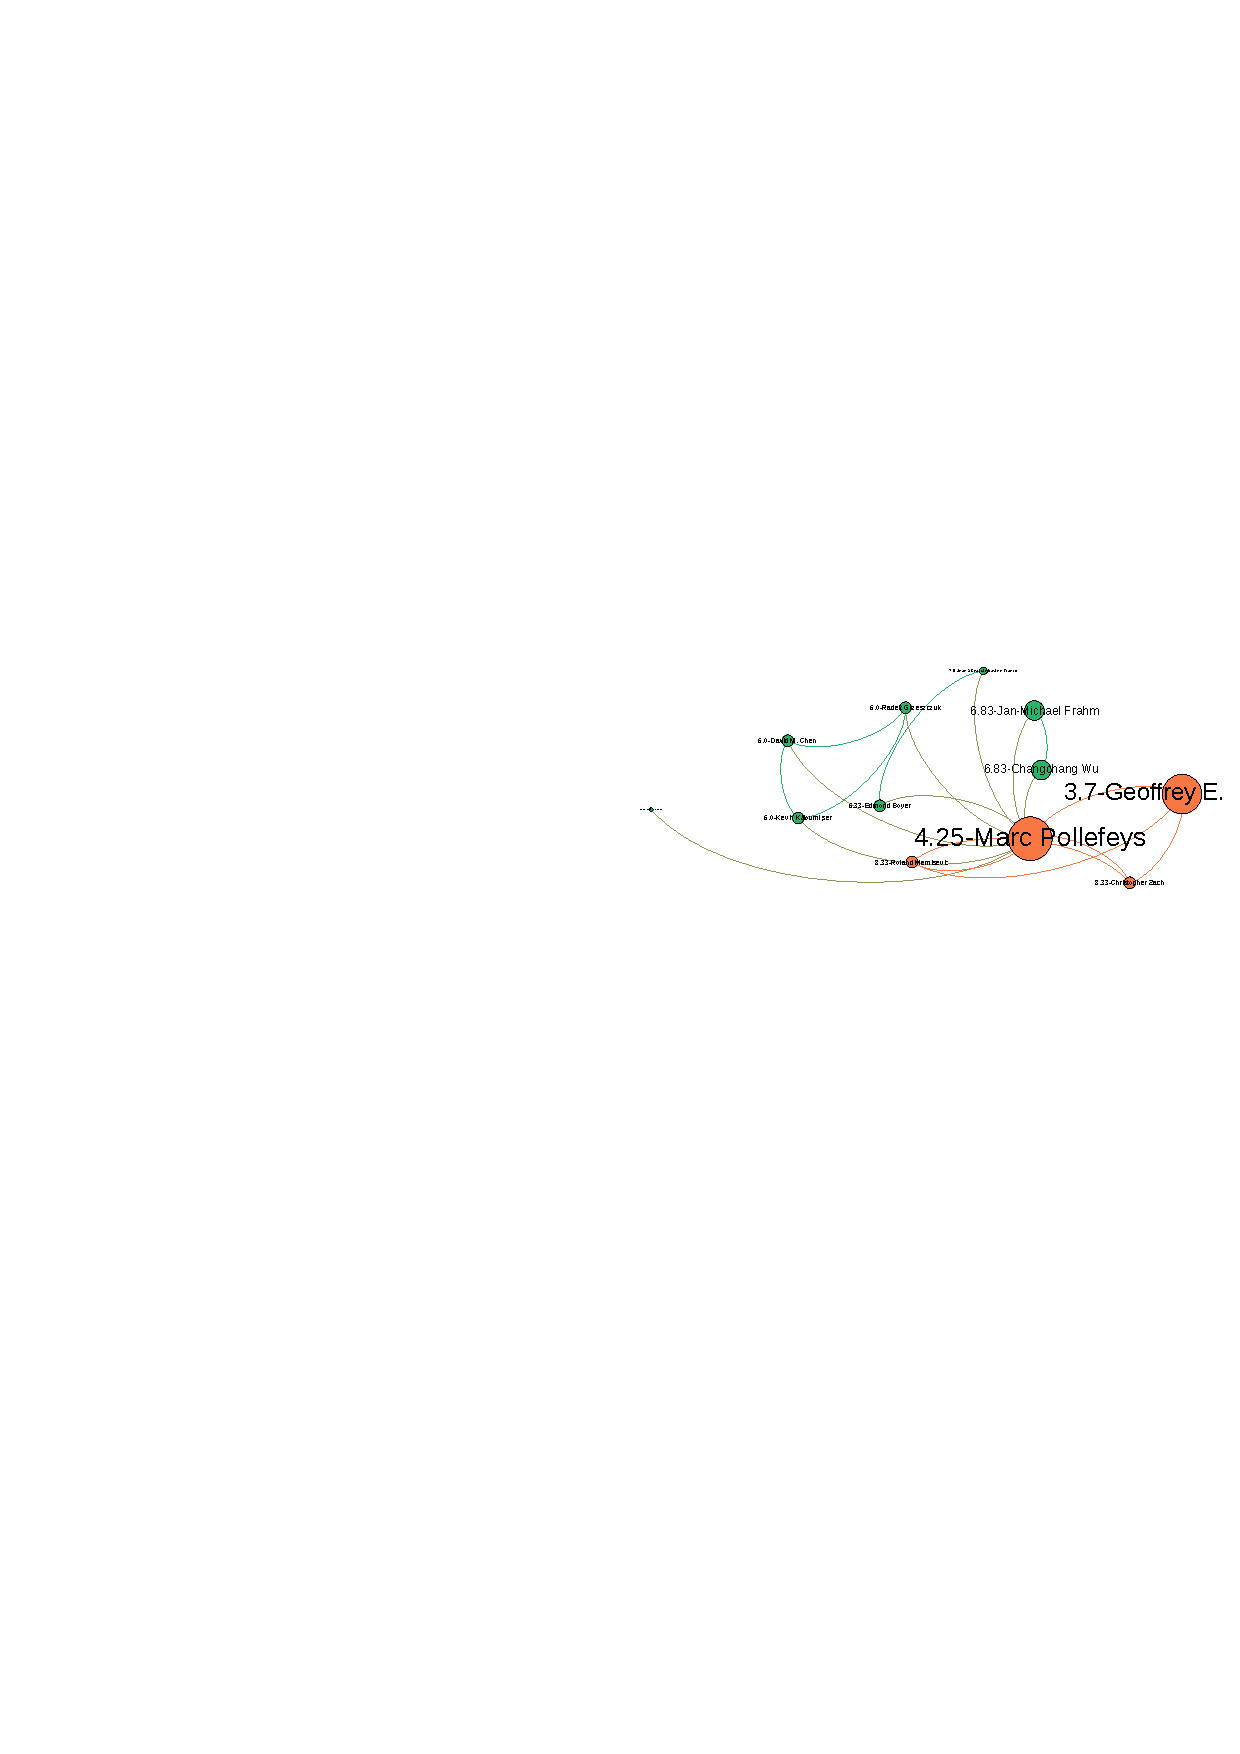
\includegraphics[width=6cm]{./figure/case0.pdf}
		\label{c}
	\end{minipage}}
	\subfigure[]{
	\begin{minipage}[t]{0.48\textwidth}
		\centering
		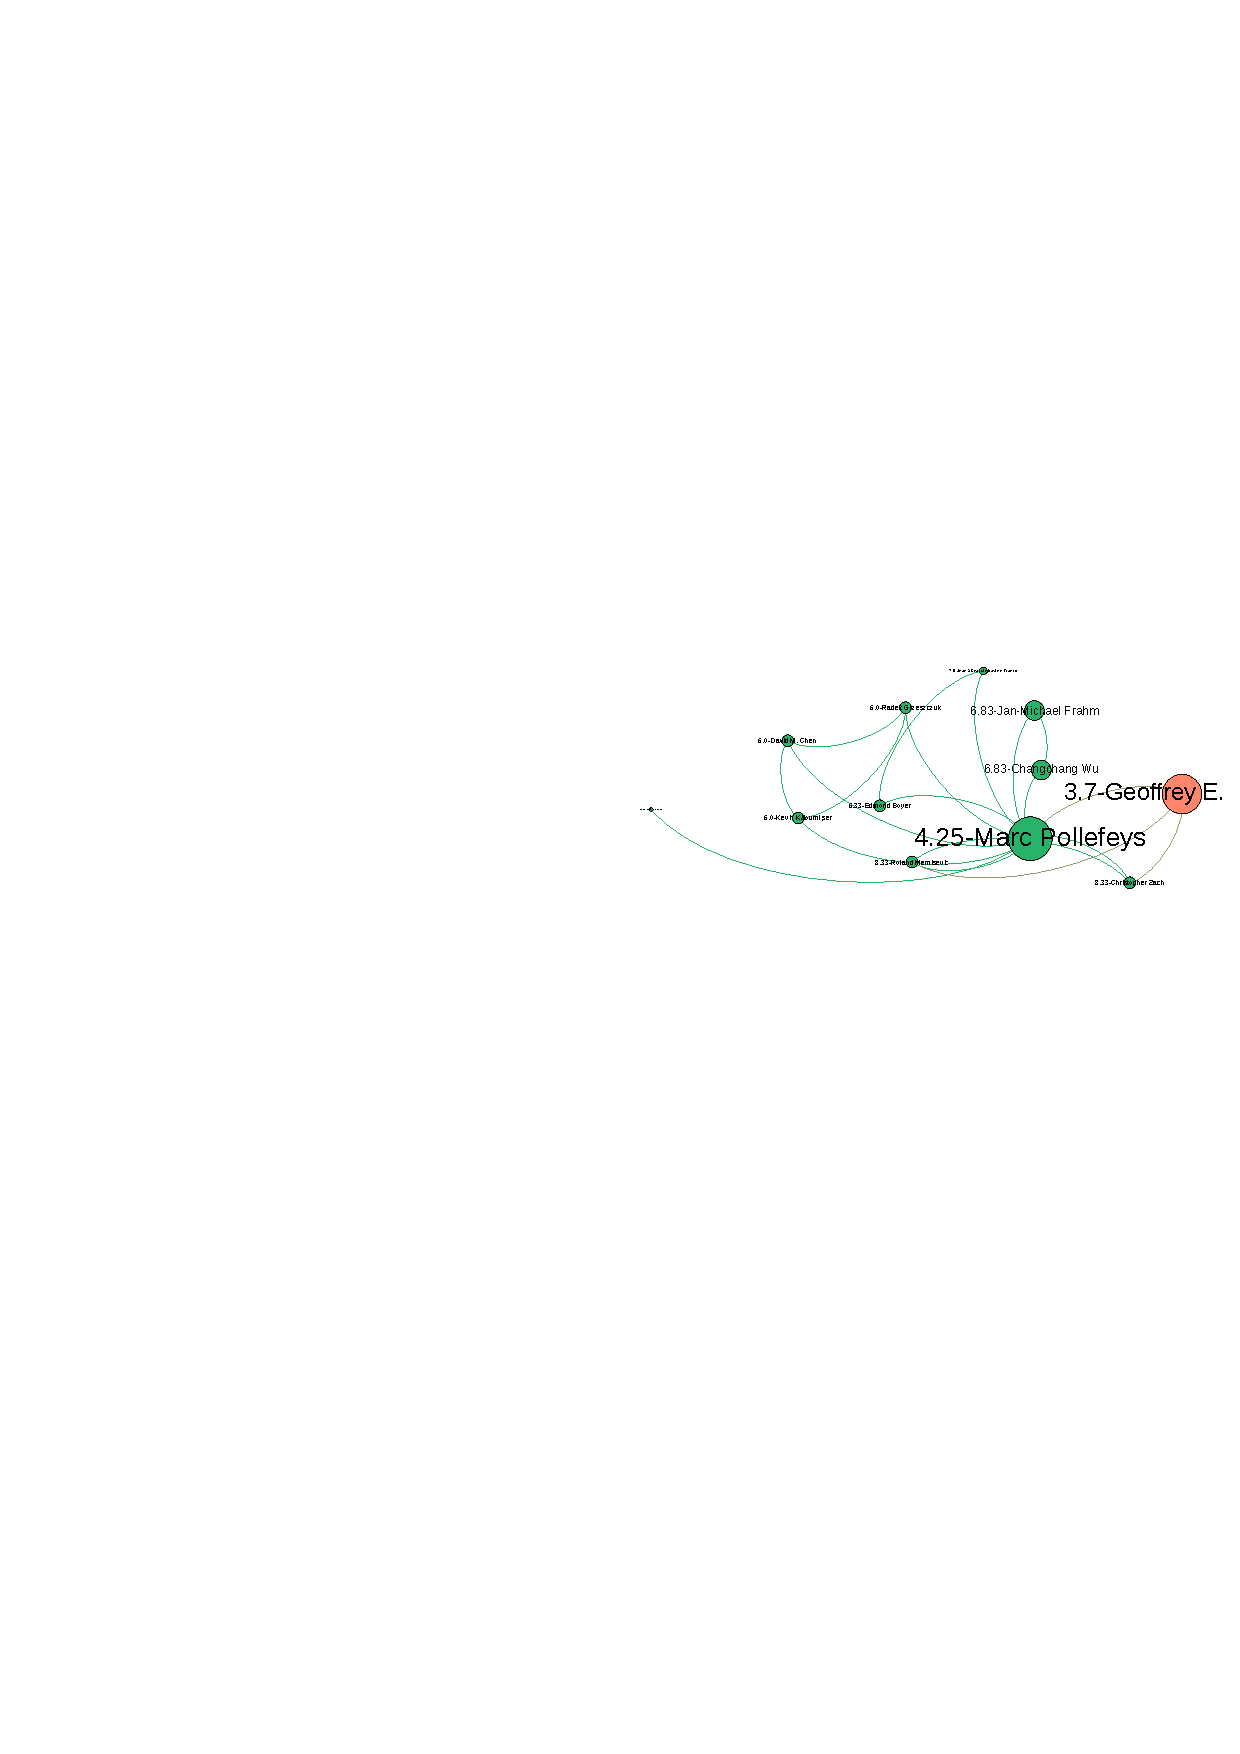
\includegraphics[width=6cm]{./figure/case1.pdf}
		\label{d}
	\end{minipage}}
	\caption{基于DBLP数据的验证案例}
	\label{fig.3.6}
\end{figure}

\section{本章小结}

通过将节点的结构属性视为分类特征,并将节点是否发生社团转移视为分类标签,本章利用决策树对其进行二分类,并分析了节点特征在分类中的重要性。最终得出结论:节点的度以及节点的平均邻居度对节点的社团转移影响最大且最为广泛。同时本章还在DBLP中找到了支撑结论的样例。下一章将会介绍受本章启发并改进自DSBM的社团检测生成模型HB-DSBM。



























\clearpage{\pagestyle{empty}\cleardoublepage}
% !Mode:: "TeX:UTF-8"
\chapter{融合节点级别社团转移参数的动态网络社团检测生成模型}

上一章介绍了利用决策树构建的框架,通过$15$个真实数据集的分析得到了影响节点社团转移的两个节点的结构属性:节点的度和节点的平均邻居度。受上一章启发,本章认为每个节点的社团转移由于其局部结构不同,都具有不同的转移倾向。而现有的动态网络社团检测模型大部分都将主要的关注点投入到了每个时间快照的社团检测上,而忽略了社团演化,小部分方法如DSBM~\cite{yang2011detecting}虽然关注了社团演化,但是其仅仅通过社团转移矩阵$A$来刻画社团演化,而忽略了每个节点的社团转移倾向的异质性,也就是说,在DSBM中,其假设同一个社团内的节点在下一个时刻发生转移的趋势都是一样的,且这种趋势在某个固定的社团内是一直不变的。这种假设在本文看来是不合理的。因此本章将会介绍引入更细粒度社团转移趋势的动态网络社团检测生成模型HB-DSBM。
\section{HB-DSBM模型构建}

\subsection{符号表示}
\begin{table}
	\centering
	\caption{HB-DSBM模型的符号表示}\label{tab.4.1}
	\begin{tabular}{cc}
		\hline
		{\bfseries 符号} &  { \bfseries 描述} \\
		\hline
		$K$,$N$,$T$ & 分别为社团个数、节点数和时间快照数 \\
		\hline
		$W^{t}$ & $t$时间快照对应的邻接矩阵\\
		\hline
		$\pi_k$ & 在时间快照$1$中,$i$节点属于社团$k$的概率\\
		$z_i^{t}$ & 在$t$快照中,$i$节点属于哪个社团 \\
		${A}_k$ & $k$社团的社团级别转移倾向 \\
		${C}_i^{t}$ & $i$节点在$t$快照中的节点级别转移倾向, 其中$t=2, \cdots, T$,$i=1, \cdots, N$\\
		$B_{kl}$ & 属于$k$社团的节点与属于$l$社团的节点在任意时间快照中的连边概率\\
		\hline
		${\gamma}$ ,${\mu}$ & ${\pi}$和${A}_k$的狄利克雷分布参数 \\
		${\alpha}$ , ${\beta}$ & $B$的Beta分布的参数 \\   
		\hline
	\end{tabular}
\end{table}

在介绍模型前,本章首先介绍模型的符号表示。如表\ref{tab.4.1}所示,本章用$W=\{W^1,W^2,...,W^T\}$表示动态网络邻接矩阵,即$W^t$表示第$t$个网络快照的邻接矩阵,其中$t \in 1,...,T$。这里$W^t \in \{0,1\}^{N\times N}$,其中$W_{ij}^t = 0$则代表$i$节点与$j$节点在网络快照$t$中没有边,若为$1$则有边。这里为了方便叙述,本章认为网络是无向无权的,这里需要说明,HB-DSBM可以有效的扩展为有向有权网络。$Z = \{Z^1,Z^2,...,Z^T\}$代表每个网络快照中节点的社团划分,例如$z_i^t = k$则表示$i$节点在网络快照$t$中属于$k$社团,其中$k\in K$。

\subsection{HB-DSBM模型}

\begin{figure}[!htbp]
	\setlength{\abovecaptionskip}{0pt} 
	\setlength{\belowcaptionskip}{10pt} 
	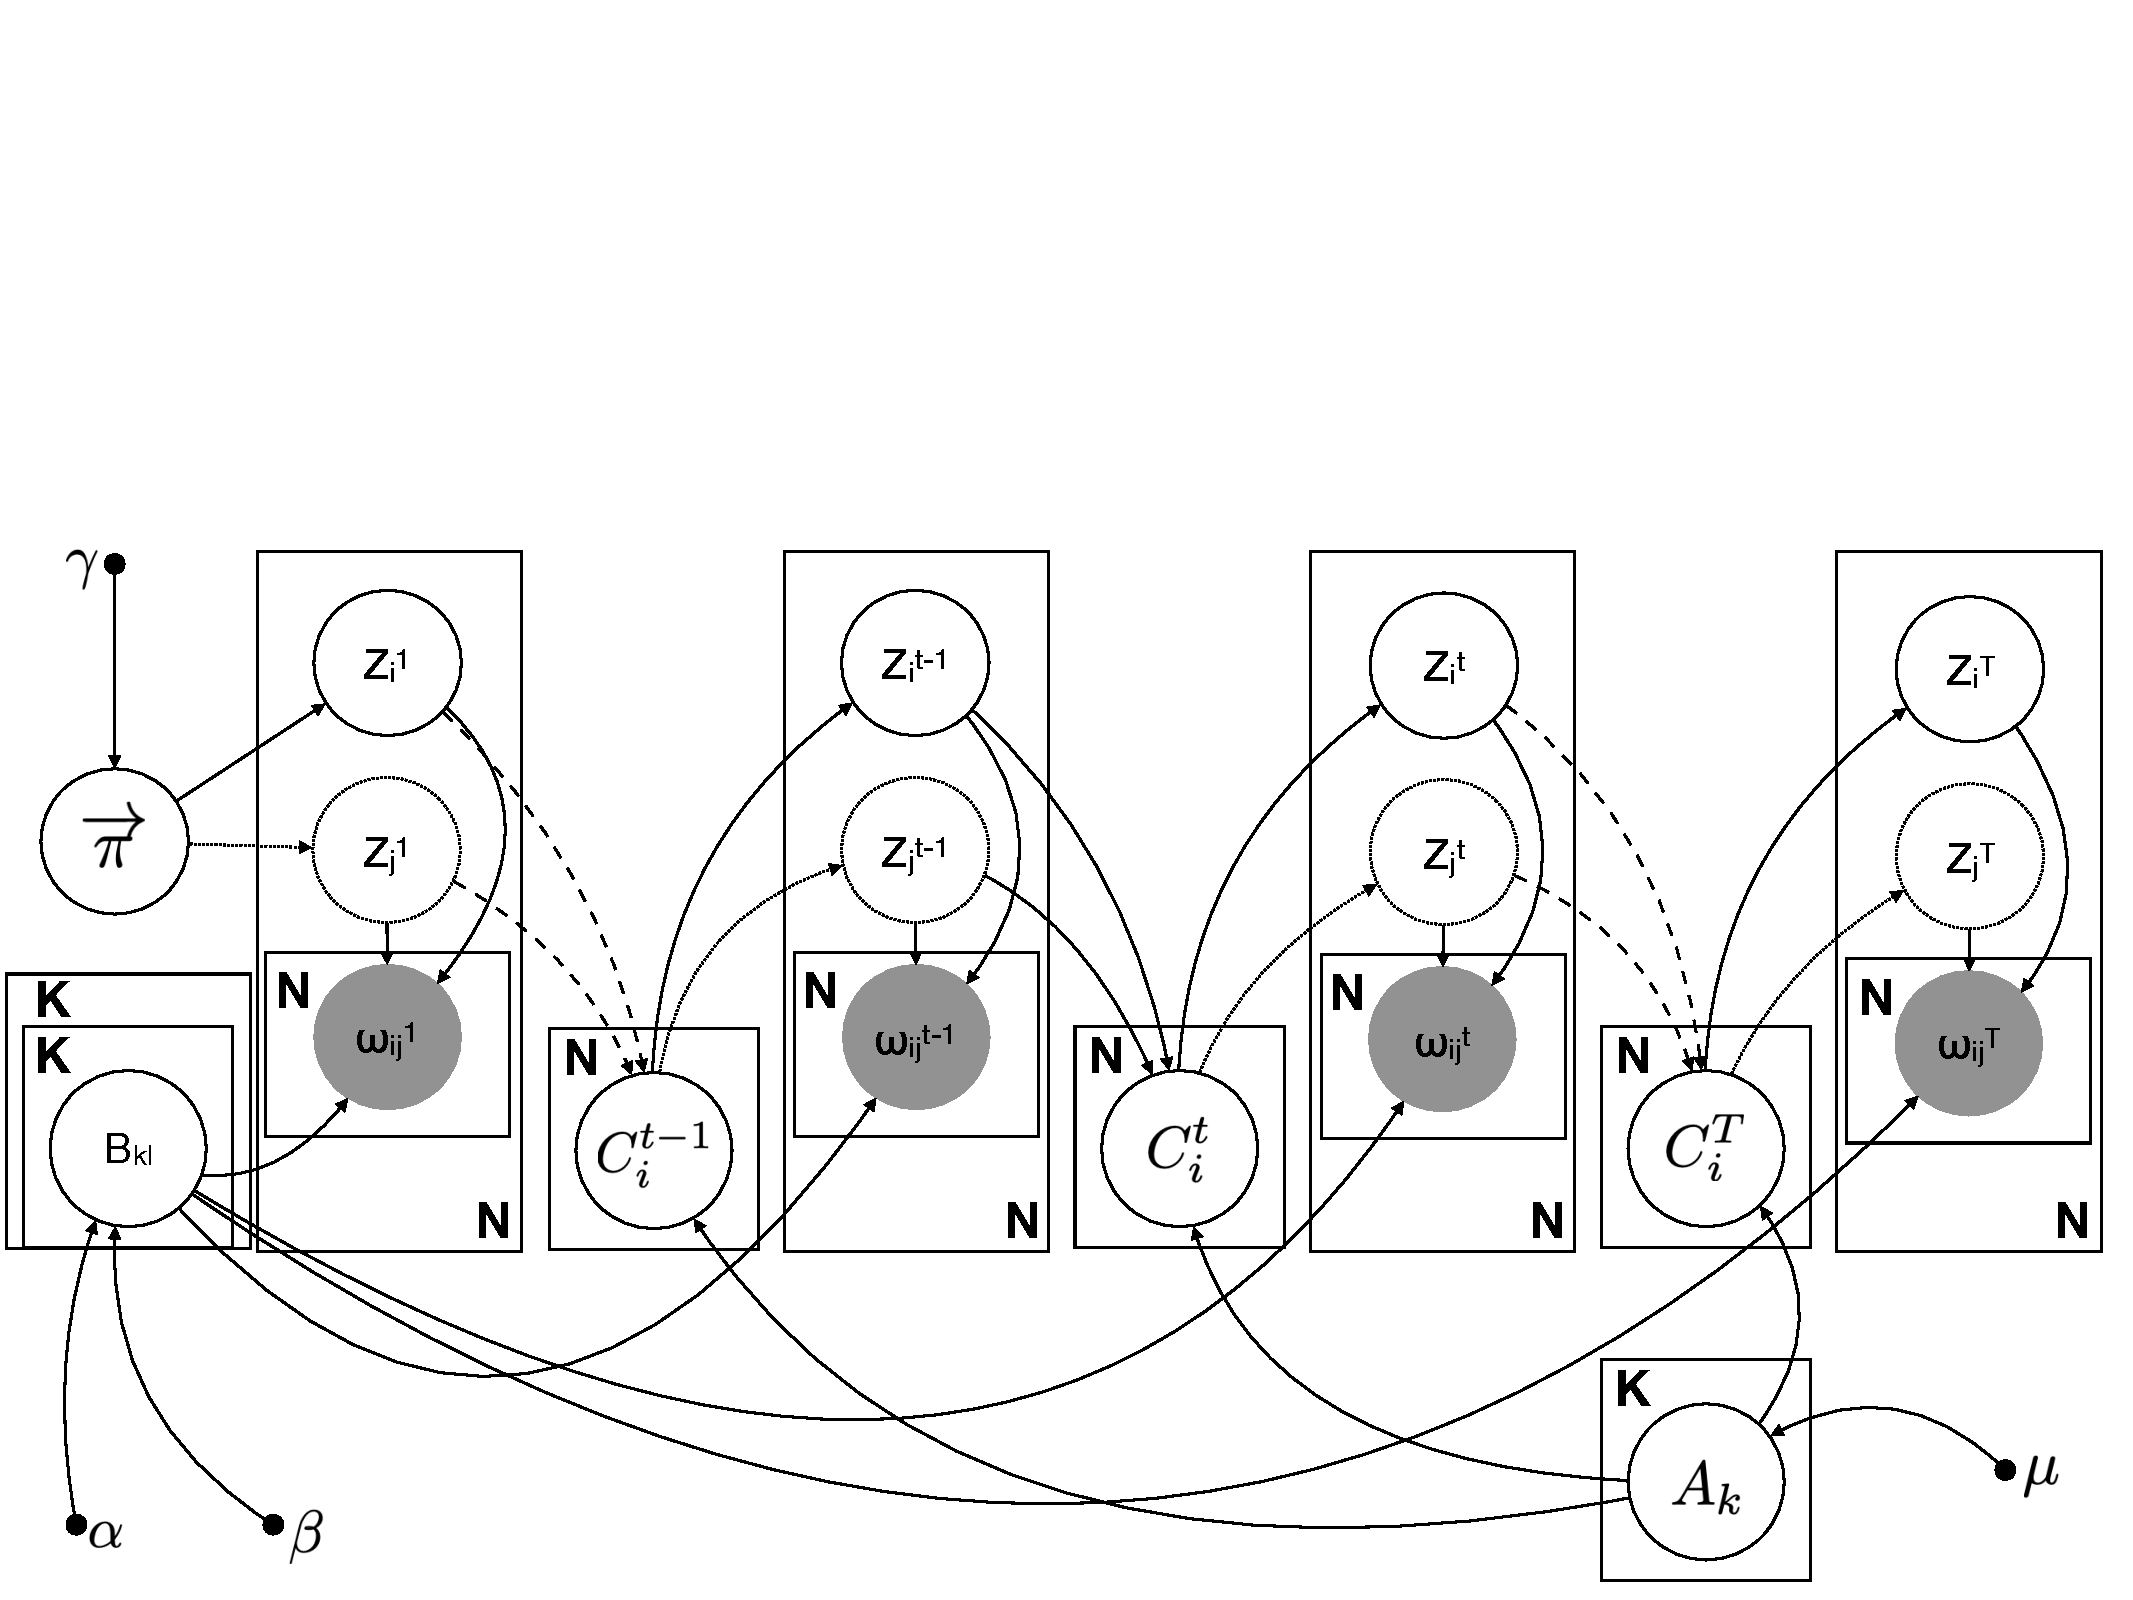
\includegraphics[width=.9\textwidth]{./figure/graph-model_v3_cuted.pdf}
	\caption{HB-DSBM图模型}
	\label{fig.4.1}
\end{figure}

本节首先介绍HB-DSBM的核心生成机制来揭示它是如何通过层次贝叶斯结构同时建模社团级别和节点级别的动态演化的,随后给出其产生社团结构和动态网络的生成过程。

如图~\ref{fig.4.1}的图模型所示,HB-DSBM首先令$\pi$表示$Z^1$的先验分布,同时$\pi$服从参数为$\gamma$的狄利克雷分布。$B$是不同社团间节点的连边概率,即类随机块模型中的块矩阵,例如$B_{kl}$即代表属于$k$社团和属于$l$社团的节点之间连边的概率。而$B$服从参数为$\alpha$和$\beta$的Beta分布。

本章中的$A \in [0, 1]^{K \times K}$表示社团级别转移倾向矩阵,$A$的每一行$A_k$都服从参数为$\mu$的狄利克雷分布,因此 $\sum_l A_{kl} = 1$。同时$C = \{ C^2, \cdots C^T \}$表示节点级别的社团转移倾向,每个$C^t$都是由社团级别转移倾向矩阵$A$生成。对于$t>1$的网络快照,任意节点$i$都有其唯一的转移向量 $C_i^t  \in [0, 1]^K$,该向量服从以参数为$A_{z_i^{t-1}}$的狄利克雷分布,因此$\sum_{k} C_{ik}^t = 1$。这一部分就是本模型的核心:层次狄利克雷生成机制。

基于以上机制,模型就可以生成社团标签以及动态网络中每个网络快照中的边。具体生成过程如下所示:
\begin{enumerate}
	\item 生成初始社团划分概率 ${\pi} \sim Dir({\gamma})$
	\item 生成块矩阵 $B \sim Beta({\alpha},{\beta})$
	\item 对于网络快照$t=1$的每个节点$i$:
	\begin{enumerate}
		\item 生成每个节点的社团归属 $z_i^1 \sim Mult({\pi})$ 
		\item 生成每条边 $\omega_{ij}^1 \sim Bernoulli(\cdot | B_{z_i^1,z_j^1})$
	\end{enumerate}
	\item 生成每个社团级别转移矩阵的社团转移向量 ${A}_k \sim Dir({\mu})$
	\item 对网络快照$t>1$中的每个节点$i$:
	\begin{enumerate}
		\item 生成每个节点级别的社团转移向量${C}_i^t \sim Dir({A}_{z_i^{t-1}})$
		\item 生成每个节点的社团归属 $z_i^t \sim Mult({C}_i^t)$
		\item 生成每条边 $\omega_{ij}^t \sim Bernoulli(\cdot | B_{z_i^t,z_j^t})$
	\end{enumerate}
\end{enumerate}

由生成过程可知,当$t=1$时,模型首先利用参数为$\pi$的多项分布生成$i$的社团归属$z_i^1$,随后以伯努利分布 $Bernoulli(\cdot|B_{z_i^1,z_j^1})$生成每对节点对$i,j$之间的连边。而当$t>1$时,$i$节点的社团归属由以参数为$C_i^t$的多项分布决定,即$z_i^t \sim Mult({C}_i^t)$。而$C_i^t$服从狄利克雷分布$Dir(A_{z_i^{t-1}})$。

根据如图~\ref{fig.4.1}的概率图模型和生成过程,可以写出HB-DSBM的联合概率分布如下:

\begin{equation}
\begin{split}
Pr&(W_T,Z_T,C_T,B,A,\pi|\alpha,\beta,\gamma,\mu) \\
= & \prod_{t=1}^T Pr(W^t | Z^t,B) Pr(Z^1|\pi) \prod_{t=2}^T Pr(Z^t|C^t) \\
& \prod_{t=2}^T Pr(C^t|A,Z^{t-1}) Pr(A|\mu) Pr(\pi|\gamma) Pr(B|\alpha,\beta) \\
\end{split}
\end{equation}

\section{模型求解}

本小结介绍针对本模型的高效的变分近似推断算法。
\subsection{变分推断}
由于模型参数较多且复杂,直接推出模型后验$p(Z,C,B,A,\pi|W)$是困难的, 因此基于平均场理论,本节提出了用$q(Z,C,B,A,\pi)$ 来近似$p(Z,C,B,A,\pi|W)$. 为了简介,本节用$\Delta$ 来表示参数 $\{\pi,B,A,C,Z\}$. 更详细来说,即:

\begin{equation}
\label{eq2}
\begin{split}
& q(\Delta) =  \prod_{t=1}^T \prod_{i=1}^N q(z_i^t) \prod_{t=2}^T \prod_{i=1}^N q(c_i^t)q(B)q(A)q(\pi)  \\
\end{split}
\end{equation}

其中块矩阵变分参数$q(B|\widetilde{\alpha},\widetilde{\beta}) = \prod_{k,l\geq k} Beta(\widetilde{\alpha}_{kl},\widetilde{\beta}_{kl})$, 社团级别转移矩阵变分参数 $q(A|\widetilde{\mu}) = \prod_{k=1}^K \prod_{l=1}^K Dir(\widetilde{\mu}_{kl})$。 而社团归属变分参数$q(z_i^t|\widetilde{\phi}_i^t)$ 服从以$\widetilde{\phi}_i^t$为参数的多项分布。
而$q(c_i^t|\widetilde{\xi}_i^t)$和$q(\pi|\widetilde{\gamma})$都分别服从以$\widetilde{\xi}_i^t$和$\widetilde{\mu}_{kl}$为参数的狄利克雷分布。

因此有变分下界:
%  \begin{equation}
%  \begin{split}
%     % & q(z_i^t|\widetilde{\phi}_i^t) \sim Multi(\widetilde{\phi}_i^t)\\
%     % & q(c_i^t|\widetilde{\xi}_i^t) \sim Dir(\widetilde{\xi}_i^t)\\
%     % & q(B|\widetilde{\alpha},\widetilde{\beta}) = \prod_{k,l\geq k} q(B_{kl}|\widetilde{\alpha}_{kl},\widetilde{\beta}_{kl})\\
%     % & q(B_{kl}|\widetilde{\alpha}_{kl},\widetilde{\beta}_{kl}) = Beta(\widetilde{\alpha}_{kl},\widetilde{\beta}_{kl}) \\
%     & q(B|\widetilde{\alpha},\widetilde{\beta}) = \prod_{k,l\geq k} Beta(\widetilde{\alpha}_{kl},\widetilde{\beta}_{kl}) \\
%     & q(A|\widetilde{\mu}) = \prod_{k=1}^K \prod_{l=1}^K Dir(\widetilde{\mu}_{kl}) \\
%     % & q(A|\widetilde{\mu}) = \prod_{k=1}^K \prod_{l=1}^K q(A_{kl} | \widetilde{\mu}_{kl})\\
%     % & q(A_{kl} | \widetilde{\mu}_{kl}) \sim Dir(\widetilde{\mu}_{kl})\\
%     % & q(\pi|\widetilde{\gamma}) = Dir(\widetilde{\gamma})\\
%  \end{split}
%  \end{equation}

\begin{equation}
\label{eq:3}
\begin{split}
&\widetilde{L}(q) = \sum_z \int_{\pi,B,A,C}q(\Delta) \log \frac{p(\Delta,W)}{q(\Delta)} 
%  \end{split}
%  \end{equation}
%  By considering the constant
%  \begin{equation}
%  \begin{split}
%      \widetilde{L}(q) = \log p(\pi,B,A,C,Z,W) - KL(q||p)
%  \end{split}
%  \end{equation}
%  
%  The ELBO is given by:
%  \begin{equation}
%  \begin{split}
= E_{\widetilde{\phi},\widetilde{\alpha},\widetilde{\beta}} \sum_{t=1}^T [\log P(W^t|Z^t,B)] \\
&+ E_{\widetilde{\gamma},\widetilde{\phi}}[\log P(Z^1|\pi)]+E_{\widetilde{\phi},\widetilde{\xi}} \sum_{t=2}^T [\log P(Z^t|C^t)] 
+ E_{\widetilde{\xi},\widetilde{\phi},\widetilde{\mu}} \sum_{t=2}^T [\log P(C^t|A,Z^{t-1})]\\
&+ E_{\widetilde{\mu}}[\log P(A)]+E_{\widetilde{\gamma}}[\log P(\pi)] + E_{\widetilde{\alpha},\widetilde{\beta}}[\log P(B)]
- E_{\widetilde{\gamma}}[\log q(\pi)] - E_{\widetilde{\alpha},\widetilde{\beta}}[\log q(B)]  - E_{\widetilde{\mu}}[\log q(A)]\\
&- \sum_{t=2}^T \sum_{i=1}^N E_{\widetilde{\xi}}[\log q(C_i^t)] - \sum_{t=1}^T \sum_{i=1}^N E_{\widetilde{\phi}}[\log q(z_i^t)] \\
\end{split}
\end{equation}

这里 $\widetilde{\phi},\widetilde{\xi},\widetilde{\alpha},\widetilde{\beta},\widetilde{\mu},\widetilde{\gamma}$ 即为变分参数。为了方便起见,本章省略掉了分布的条件部分。 例如,本章将 $q(\Delta|\widetilde{\phi},\widetilde{\xi},\widetilde{\alpha},\widetilde{\beta},\widetilde{\mu},\widetilde{\gamma})$ 和 $q(z_i^t|\widetilde{\phi}_i^t)$ 略写为$q(\Delta)$和$q(z_i^t)$。
因此该模型的变分下界(ELBO)$\widetilde{L}(q)$被写成了如上式\ref{eq:3}。

随后通过最大化ELBO来获得最优的隐变量$Z,\pi,B,A,C$和模型参数$\gamma,\alpha,\beta,\mu$。 通过对不同的参数$\widetilde{\phi},\widetilde{\gamma},\widetilde{\alpha},\widetilde{\beta},\widetilde{\mu},\widetilde{\xi}$对$\widetilde{L}(q)$求偏导,并令导数为0求得每个参数的更新公式,即:
\begin{equation}
\begin{split}
\nabla \widetilde{L}(q) = \{ \frac{\partial \widetilde{L}}{\partial \widetilde{\gamma}},\frac{\partial \widetilde{L}}{\partial \widetilde{\alpha}},\frac{\partial \widetilde{L}}{\partial \widetilde{\beta}},\frac{\partial \widetilde{L}}{\partial \widetilde{\mu}},\frac{\partial \widetilde{L}}{\partial \widetilde{\xi}},\frac{\partial \widetilde{L}}{\partial \widetilde{\phi}} \} = 0
\end{split}
\end{equation}

每个参数的结果如下所示:
\textbf{对 $\widetilde{\gamma}$}:

包含$\widetilde{\gamma}$的ELBO如下所示:
\begin{equation}
\begin{split}
& \widetilde{L}_{\widetilde{\gamma}} = E_{\widetilde{\gamma},\widetilde{\phi}}[\log P(Z^1|\pi)] + E_{\widetilde{\gamma}}[\log P(\pi)]- E_{\widetilde{\gamma}}[\log q(\pi)] \\
& = \log{\frac{\prod_{k=1}^K \log \Gamma (\widetilde{\gamma}_k)}{\Gamma (\sum_k \widetilde{\gamma}_k)}} 
 + \sum_{k=1}^K ( \gamma_k - \widetilde{\gamma}_k + \sum_{i=1}^N \widetilde{\phi}_{ik}^1)[\psi(\widetilde{\gamma}_k) - \psi(\sum_k \widetilde{\gamma}_k)]\\
\end{split}
\end{equation}

这里 $\psi(x) = \frac{\Gamma'(x)}{\Gamma(x)} = \frac{\,d \log \Gamma(x)}{\, dx}$. 
通过对$\widetilde{L}_{\widetilde{\gamma}}$ 针对$\widetilde{\gamma}$求偏导,并令导数等于0,得到其更新公式如下:
\begin{equation}
\label{eq4}
\begin{split}
\widetilde{\gamma}_k = \gamma_k + \sum_{i=1}^N \widetilde{\phi}_{ik}^1, \quad
% \widetilde{\mu}_{kl} \propto \mu_l + \frac{\sum_{t=2}^T \sum_i \widetilde{\phi}_{ik}^{t-1}}{T-1}
\end{split}
\end{equation}

\textbf{对于$\widetilde{\xi}$}:

ELBO中包含$\widetilde{\xi}$的式子如下所示:
\begin{equation}
\begin{split}
&\widetilde{L}_{\widetilde{\xi}} = E_{\widetilde{\phi},\widetilde{\xi}} \sum_{t=2}^T [\log P(Z^t|C^t)] 
+ E_{\widetilde{\xi},\widetilde{\phi},\widetilde{\mu}} \sum_{t=2}^T [\log P(C^t|A,Z^{t-1})] - \sum_{t=2}^T \sum_{i=1}^N E_{\widetilde{\xi}}[\log q(C_i^t)]\\
\end{split}
\end{equation}

利用同样方法求得更新公式如下所示:

\begin{equation}
\label{eq5}
\begin{split}
\widetilde{\xi}_{ik}^t \propto \widetilde{\phi}_{ik}^t + \sum_l \widetilde{\phi}_{il}^{t-1}(\frac{\widetilde{\mu}_{kl}}{\sum_l \widetilde{\mu}_{kl}} - 1) + 1
\end{split}
\end{equation}

\textbf{对于参数$\widetilde{\alpha}$和$\widetilde{\beta}$}:

ElBO中包含$\widetilde{\alpha}$和$\widetilde{\beta}$的式子如下所示:
\begin{equation}
\begin{split}
&\widetilde{L}_{\widetilde{\alpha},\widetilde{\beta}} = E_{\widetilde{\phi},\widetilde{\alpha},\widetilde{\beta}} \sum_{t=1}^T [\log P(W^t|Z^t,B)] 
- E_{\widetilde{\alpha},\widetilde{\beta}}[\log q(B)] + E_{\widetilde{\alpha},\widetilde{\beta}}[\log P(B)]\\
&= \sum_{k \leq l} \log\{\frac{\Gamma(\widetilde{\alpha}_{kl})\Gamma(\widetilde{\beta}_{kl})}{\Gamma(\widetilde{\alpha}_{kl}+\widetilde{\beta}_{kl})}   \}  \\
&+ \sum_{k=1}^K [\alpha_{kk}- \widetilde{\alpha}_{kk} +\sum_t \sum_{i < j} \widetilde{\phi}_{ik}^t\widetilde{\phi}_{jk}^t w_{ij}^t]
[\psi(\widetilde{\alpha}_{kk})-\psi (\widetilde{\alpha}_{kk}+\widetilde{\beta}_{kk})] \\
&+ \sum_{k=1}^K [\beta_{kk}- \widetilde{\beta}_{kk} +\sum_t \sum_{i < j} \widetilde{\phi}_{ik}^t\widetilde{\phi}_{jk}^t(1- w_{ij}^t)]
[\psi(\widetilde{\beta}_{kk})-\psi (\widetilde{\alpha}_{kk}+\widetilde{\beta}_{kk})] \\
&+ \sum_{k<l}^K [\alpha_{kl}- \widetilde{\alpha}_{kl} +\sum_t \sum_{i \neq j} \widetilde{\phi}_{ik}^t\widetilde{\phi}_{jk}^t w_{ij}^t]
[\psi(\widetilde{\alpha}_{kl})-\psi (\widetilde{\alpha}_{kl}+\widetilde{\beta}_{kl})] \\
&+ \sum_{k<l}^K [\beta_{kl}- \widetilde{\beta}_{kl} +\sum_t \sum_{i \neq j} \widetilde{\phi}_{ik}^t\widetilde{\phi}_{jk}^t(1- w_{ij}^t)]
[\psi(\widetilde{\beta}_{kl})-\psi (\widetilde{\alpha}_{kl}+\widetilde{\beta}_{kl})] \\
\end{split}
\end{equation}

利用同样方法求得$\widetilde{\alpha}$和$\widetilde{\beta}$的更新公式如下:

\begin{equation}
\label{eq6}
\begin{split}
& \widetilde{\alpha}_{kk} = \alpha_{kk} + \frac{\sum_t \sum_{i<j} \widetilde{\phi}_{ik}^t \widetilde{\phi}_{jk}^t w_{ij}^t}{T}  \\
& \widetilde{\beta}_{kk} = \beta_{kk} + \frac{\sum_t \sum_{i<j} \widetilde{\phi}_{ik}^t \widetilde{\phi}_{jk}^t (1-w_{ij}^t)}{T} \\
& \widetilde{\alpha}_{kl} = \alpha_{kl} + \frac{\sum_t \sum_{i \neq j} \widetilde{\phi}_{ik}^t \widetilde{\phi}_{jl}^t w_{ij}^t}{T} \\
& \widetilde{\beta}_{kl} = \beta_{kl} + \frac{\sum_t \sum_{i \neq j} \widetilde{\phi}_{ik}^t \widetilde{\phi}_{jl}^t (1-w_{ij}^t)}{T}  \\
\end{split}
\end{equation}

\textbf{对于 $\widetilde{\mu}$}:

ELBO中包含$\widetilde{\mu}$的式子如下所示:

\begin{equation}
\begin{split}
& \widetilde{L}_{\widetilde{\mu}} = E_{\widetilde{\xi},\widetilde{\phi},\widetilde{\mu}} \sum_{t=2}^T [\log P(C^t|A,Z^{t-1})] 
- E_{\widetilde{\mu}}[\log q(A)]+ E_{\widetilde{\mu}}[\log P(A)]\\
&=\sum_{t=2}^T \sum_i \sum_k \sum_l \widetilde{\phi}_{ik}^{t-1} [\sum_l \psi(\widetilde{\mu}_{kl}) - \psi(\sum_l \widetilde{\mu}_{kl}) 
+ \frac{\widetilde{\mu}_{kl}}{\sum_l \widetilde{\mu}_{kl}}(\psi(\widetilde{\xi}_{ik}^t)-\psi(\sum_l \widetilde{\xi}_{il}^t))]  \\
&-\log[\Gamma(\sum_l \widetilde{\mu}_{kl})] + \sum_l \log[\Gamma(\widetilde{\mu}_{kl})]
+ \sum_l (\mu_l - \widetilde{\mu}_{kl})[\psi(\widetilde{\mu}_{kl}) - \psi(\sum_l \widetilde{\mu}_{kl})]  \\
\end{split}
\end{equation}

因此有:
\begin{equation}
\label{eq7}
\begin{split}
\widetilde{\mu}_{kl} \propto \mu_l + \frac{\sum_{t=2}^T \sum_i \widetilde{\phi}_{ik}^{t-1}}{T-1}
\end{split}
\end{equation}

\textbf{对于 $\widetilde{\phi}$}:

$\widetilde{\phi}$ 是社团划分参数$Z$的变分参数,其更新公式随$t$的不同而不同。下面分情况讨论:

\textbf{当$t=1$时}:

ELBO中包含$\widetilde{\phi}$的项并考虑约束$\sum_k \widetilde{\phi}_{ik} = 1$,有:

\begin{equation}
\begin{split}
&\widetilde{L}_{\widetilde{\phi}} = E_{\widetilde{\phi},\widetilde{\alpha},\widetilde{\beta}} [\log P(W^1|Z^1,B)] + E_{\widetilde{\gamma},\widetilde{\phi}}[\log P(Z^1|\pi)] \\
&+ E_{\widetilde{\xi},\widetilde{\phi},\widetilde{\mu}}[\log P(C^2|A,Z^1)] - E_{\widetilde{\phi}}[\log q(Z^1)]+\rho (\sum_k \widetilde{\phi}_{ik}-1)\\
\end{split}
\end{equation}

因此有:

%Here $\phi$ is the variational parameter of $Z$ with $T$ snapshot, we get the update rules of $\phi$ at different snapshots $t$ as follows.
%When $t=1$:
\begin{equation}
\label{eq8}
\begin{split}
&\widetilde{\phi}_{ik}^1 \propto \exp\{\sum_j \sum_l \widetilde{\phi}_{jl}^1 [w_{ij}^1[\psi(\widetilde{\alpha}_{kl})-\psi(\widetilde{\alpha}_{kl}+\widetilde{\beta}_{kl})]
  + (1-w_{ij}^1)[\psi(\widetilde{\beta}_{kl}) - \psi(\widetilde{\alpha}_{kl}+\widetilde{\beta}_{kl})] ]   \\
& +[\psi(\widetilde{\gamma}_k)-\psi(\sum_l \widetilde{\gamma}_l) ] +[\sum_l \psi(\widetilde{\mu}_{kl}) - \psi(\sum_l \widetilde{\mu}_{kl}) 
+ \sum_l (\frac{\widetilde{\mu}_{kl}}{\sum_l \widetilde{\mu}_{kl}}-1)(\psi (\widetilde{\xi}_{ik}^2) - \psi(\sum_l \widetilde{\xi}_{il}^2))]  \} \\
\end{split}
\end{equation}

\textbf{当$1<t<T$}:

ELBO中包含$\widetilde{\phi}$的项,同时考虑$\sum_k \widetilde{\phi}_{ik} = 1 $,有:

\begin{equation}
\begin{split}
& \widetilde{L}_{\widetilde{\phi}} = E_{\widetilde{\phi},\widetilde{\alpha},\widetilde{\beta}} [\log P(W^t|Z^t,B)]+E_{\widetilde{\phi},\widetilde{\xi}} [\log P(Z^t|C^t)]\\
&+  E_{\widetilde{\xi},\widetilde{\phi},\widetilde{\mu}} [\log P(C^{t+1}|A,Z^t)]- \sum_{i=1}^N E_{\widetilde{\phi}}[\log q(z_i^t)]\\
\end{split}
\end{equation}
%When $1<t<T$:
因此有:
\begin{equation}
\label{eq9}
\begin{split}
&\widetilde{\phi}_{ik}^t \propto \exp \{ \sum_j \sum_l \widetilde{\phi}_{jl}^t [w_{ij}^t[\psi(\widetilde{\alpha}_{kl}) - \psi(\widetilde{\alpha}_{kl}+\widetilde{\beta}_{kl})]
+ (1-w_{ij}^t)[\psi(\widetilde{\beta}_{kl})-\psi(\widetilde{\alpha}_{kl}+\widetilde{\beta}_{kl})]]    \\
& + [\psi(\widetilde{\xi}_{ik}^t) - \psi(\sum_l \widetilde{\xi}_{il}^t)]+ [\sum_l \psi(\widetilde{\mu}_{kl}) - \psi(\sum_l \widetilde{\mu}_{kl}) 
+\sum_l (\frac{\widetilde{\mu}_{kl}}{\sum_l \widetilde{\mu}_{kl}} -1)(\psi(\widetilde{\xi}_{ik}^{t+1}) - \psi(\sum_l \widetilde{\xi}_{il}^{t+1}))]  \}\\
\end{split}
\end{equation} 

\textbf{当$t=T$}:

ELBO中包含$\widetilde{\phi}$的项同时考虑约束$\sum_k \widetilde{\phi}_{ik} = 1 $,有:

\begin{equation}
\begin{split}
& \widetilde{L}_{\widetilde{\phi}} = E_{\widetilde{\phi},\widetilde{\alpha},\widetilde{\beta}} [\log P(W^T|Z^T,B)]+E_{\widetilde{\phi},\widetilde{\xi}} [\log P(Z^T|C^T)]
- \sum_{i=1}^N E_{\widetilde{\phi}}[\log q(z_i^T)]\\
\end{split}
\end{equation}
%   When $t=T$:
因此有:
\begin{equation}
\label{eq10}
\begin{split}
&\widetilde{\phi}_{ik}^T \propto \exp \{ \sum_j \sum_l \widetilde{\phi}_{jl}^T [w_{ij}^T[\psi(\widetilde{\alpha}_{kl}) - \psi(\widetilde{\alpha}_{kl}+\widetilde{\beta}_{kl})] + \\
&(1-w_{ij}^T)[\psi(\widetilde{\beta}_{kl})-\psi(\widetilde{\alpha}_{kl}+\widetilde{\beta}_{kl})]]  + [\psi(\widetilde{\xi}_{ik}^T) - \psi(\sum_l \widetilde{\xi}_{il}^T)]\}  \\
\end{split}
\end{equation} 
% Here $\psi(x) = \frac{\Gamma'(x)}{\Gamma(x)} = \frac{\,d \log \Gamma(x)}{\, dx}$. 

由更新公式可知,模型超参数$\mu$和$\alpha$ 都为常量且其不影响模型结果。下面介绍得到更新公式后的迭代算法

\subsection{迭代算法}

现在已经有了所有参数的更新公式,下面给出变分EM的更新算法如算法~\ref{alg4.1}所示。

\begin{algorithm}
	\caption{HB-DSBM迭代算法}\label{alg4.1}
	\algorithmicrequire ~~ 动态网络邻接矩阵 $W$, 对大迭代次数 $n_{max}$ 和阈值变量$\varepsilon$ \\
	\algorithmicensure ~~ $\widetilde{\alpha},\widetilde{\beta},\widetilde{\gamma},\widetilde{\mu},\widetilde{\xi},\widetilde{\phi}$
	\begin{algorithmic}[1]
		\REPEAT
		\STATE 给定$\widetilde{\phi}$, 根据迭代公式~\ref{eq4}
		~\ref{eq5}~\ref{eq6}~\ref{eq7}更新 $\widetilde{\xi},\widetilde{\gamma},\widetilde{\alpha},\widetilde{\beta},\widetilde{\mu}$
		\STATE 给定 $\widetilde{\xi},\widetilde{\gamma},\widetilde{\alpha},\widetilde{\beta},\widetilde{\mu}$, 根据迭代公式\ref{eq8}~\ref{eq9}~\ref{eq10}更新 $\widetilde{\phi}$ 
		\UNTIL {$|\mathcal{L}^{new}-\mathcal{L}^{old}|<\varepsilon$ 或迭代次数 $> n_{max}$}
		\RETURN $\widetilde{\xi},\widetilde{\gamma},\widetilde{\alpha},\widetilde{\beta},\widetilde{\mu},\widetilde{\phi}$
	\end{algorithmic}
\end{algorithm}

算法的复杂度依赖于三个部分。 更新$\phi$的复杂度是$O(TN^2K^2)$, 其中 $T$ 是网络快照的个数,  $N$ 网络中节点的数量,而$K$ 是社团的个数。 而更新 $\xi$的复杂度是$O(TNK^2)$。 最后ELBO的计算复杂度是$O(TN^2K^2)$.因此理论上该算法的复杂度是 $O(N^2)$. 而真实世界网络的数据往往是稀疏的,因此可以通过负采样或并行计算有效提升算法的运行效率,使其适应于大规模数据集。

\section{实验及验证}

本小结将本文提出的算法HB-DSBM与四种同类动态网络社团检测算法在四个数据集(两个生成数据集与两个真实数据集)进行比较,以证明HB-DSBM的效果优于同类方法。同时在DBLP数据集中对HB-DSBM与DSBM进行社团演化分析,以证明本方法的社团演化分析更加细致且符合实际。
\subsection{数据集}
本章实验使用四个数据集对HB-DSBM及对比方法进行比较,包括两个生成数据集和两个真实数据集,所有数据集均有真相。

\textbf{data1} 由Lin 等人~\cite{lin2008facetnet}基于Girvan 和Newman提出的数据的改进版数据集。该数据集具有不同的参数设置,每个参数设置组生成的数据包含$10$个时间快照和$128$个节点,这些节点分别属于$4$个不同的社团,每个社团均包含32个节点。参数$\sigma$表示某社团内部的节点与其他社团的节点连边的数量的均值;而$nC$代表每个时间快照到下一个时间快照离开其原有社团的节点的数量;$aD$则表示每个节点的平均度。

\textbf{data2}是由Greene等人\cite{greene2010tracking}提出的。该数据集融合了社团级别的事件使得其更接近真实世界数据,该数据集中的每个网络包含$1000$个节点,$15$的平均度和$50$的最大节点度。该数据集的社团个数有$20$到$50$不等,社团间连边的概率为$0.2$。值得一提的是,该数据集中的节点服从网络的power-law。

\textbf{KIT-email}\cite{gorkedynamic}数据集是email收发网络,其节点代表电子邮箱账号。本文将该数据集视作无向无权网络,并将该数据集处理成网络快照形式的数据,分别以$2$或$3$个月为一个时间间隔。其节点数以及社团个数对应于这两个时间间隔分别为$138$、$170$和$23$、$25$。

\textbf{DBLP}\cite{konect:2017:dblp-cite}数据是开源的论文数据集。本文选取了涉及计算机的三个领域的数据,包括数据挖掘(DM)、数据库(DB)和人工智能(AI)。时间跨度为$9$年,其中包括$1163$个节点和按领域划分的$3$个社团。本文将数据划分为$9$个网络快照,每个快照对应一年。

\subsection{动态社团检测}
本小结社团检测实验选取了四种动态网络社团检测方法,分别为DSBM~\cite{yang2011detecting}、DYNMOGA~\cite{folino2014evolutionary}、Genlouvain~\cite{jutla2011generalized}和PisCES~\cite{liu2018global},这四种动态社团检测方法均为不同实现方式得到的高质量的动态网络社团检测算法。以上四个算法的参数设置均遵从其原论文的设置。而HB-DSBM的超参数如前文所述,均对模型效果影响不大,因此实验部分设置参数为当$k \neq l$时 $\alpha_{kl} = 1$,而当$k \neq l$时 $\alpha_{kk} = 10$;$\beta$的设置与$\alpha$相同; $\mu$的设置和$\gamma$相同, 即 $\mu_k = \gamma_k = \frac{1}{K}$,其中$1<k<K$。
\subsubsection{评价指标}
本章实验部分使用标准化互信息指标(NMI)~\cite{gong2007machine}作为社团检测效果的评价指标,这也是目前大部分动态社团检测方法所使用的评价指标。NMI被设计为静态网络社团划分的评价指标,因此本章会在每个时间快照计算社团划分的NMI值。NMI被用作网络社团划分衡量指标需要知道网络社团划分的真相。令$C=\{C_1,...,C_K\}$表示网络社团划分的真相,令 $C'=\{C'_1,...,C'_K\}$代表待评估的社团划分,其中$C_k$和$C'_k$分别代表真相以及待评估的第$k$个社团的所有节点。则NMI的定义如下所示:

\begin{equation}
\begin{split}
NMI(C,C')=\frac{\sum_{C,C'}p(C,C')\log \frac{p(C,C')}{p(C)p(C')}}{max(H(C)H(C'))}
\end{split}
\end{equation}

其中,$H(C)$和$H(C')$表示社团$C$和$C'$的熵。NMI的值在$0$到$1$之间。NMI的值越高,代表待评估的社团划分与真相越接近。



\subsubsection{实验结果}

将HB-DSBM与DYNOMGA、DSBM、GenLou以及PisCES在不同数据集中进行NMI对比。在$data1$不同参数设置中的对比结果如图~\ref{fig.4.2}所示,HB-DSBM在图~\ref{fig.4.2}(a)中比效果最好的DSBM有大约明显的NMI提升,同时在图~\ref{fig.4.2}(d)中有$0.1$的NMI提升。虽然HB-DSBM在图~\ref{fig.4.2}(b)与图~\ref{fig.4.2}(c)中与其余方法的NMI提升差距不大,但是依然是效果最好的。HB-DSBM在五中方法中具有最好的NMI效果,证明该方法正确的把握住了节点演化的模式。HB-DSBM的曲线更加平滑,因为该模型结合了社团级别的演化以及节点级别的演化模式,成功的把握住了节点演化的异质性。DSBM的NMI曲线也比其他方法更加平滑,因为其融合了社团级别的演化模式,但是其忽略了同社团节点内演化模式的异质性。反观DYNOMGA和GenLou将社团检测与社团演化看做了两个独立的部分,因此其NMI曲线不够平滑,特别是在图~\ref{fig.4.2}(c)和图~\ref{fig.4.2}(d)中。而PisCES在不同时间快照中显示了很大的NMI反差,说明其对网络的噪声非常敏感。

\begin{figure}[htbp]
	\centering
	\subfigure[$\sigma=4,nC=9,aD=16$]{
		\label{Fig.4.2.a}
		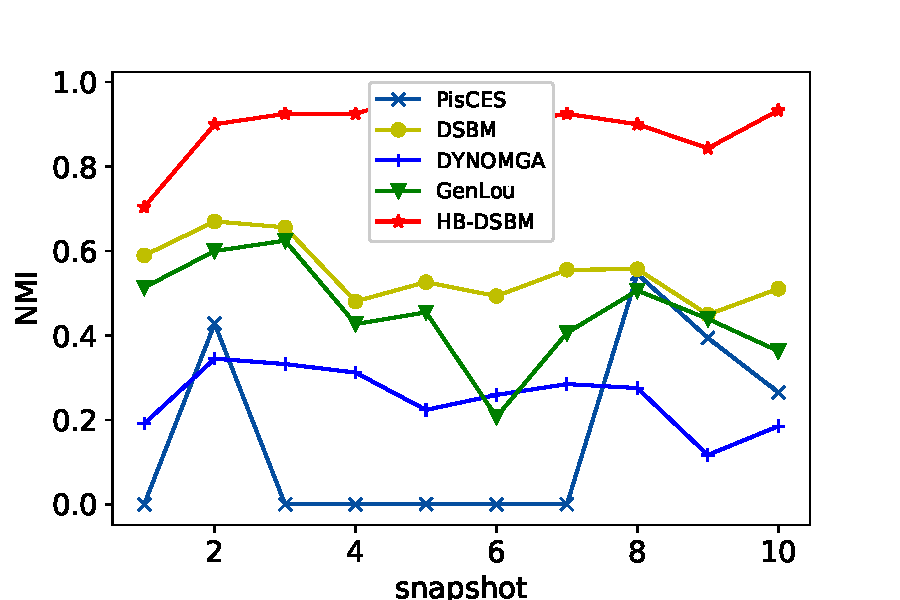
\includegraphics[width=.48\textwidth]{./figure/compare4916.pdf}
	}
	\subfigure[$\sigma=4,nC=9,aD=20$]{
		% \label{Fig.vis.1}
		\label{Fig.4.2.b}
		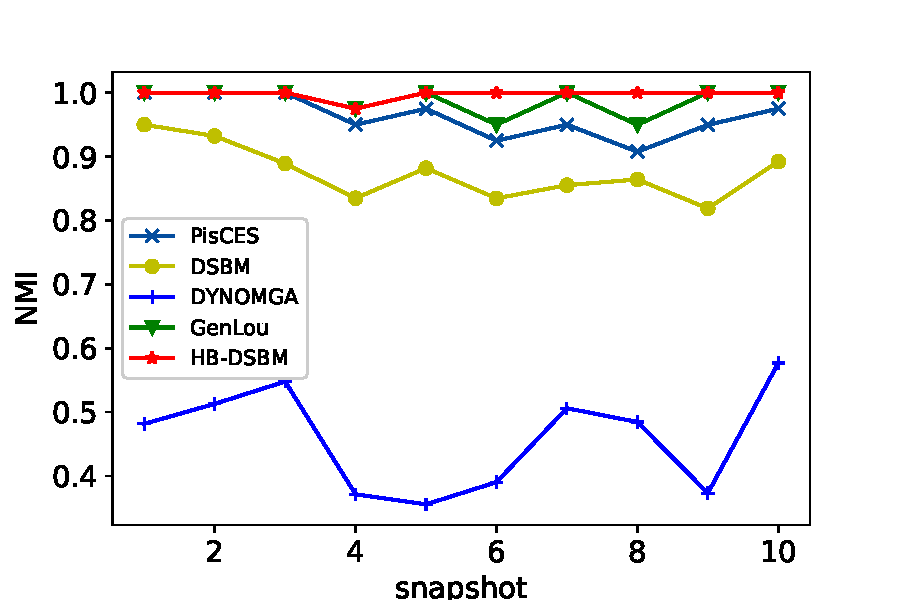
\includegraphics[width=.48\textwidth]{./figure/compare4920.pdf}
	}
	\subfigure[$\sigma=5,nC=3,aD=16$]{
		% \label{Fig.vis.1}
		\label{Fig.4.2.c}
		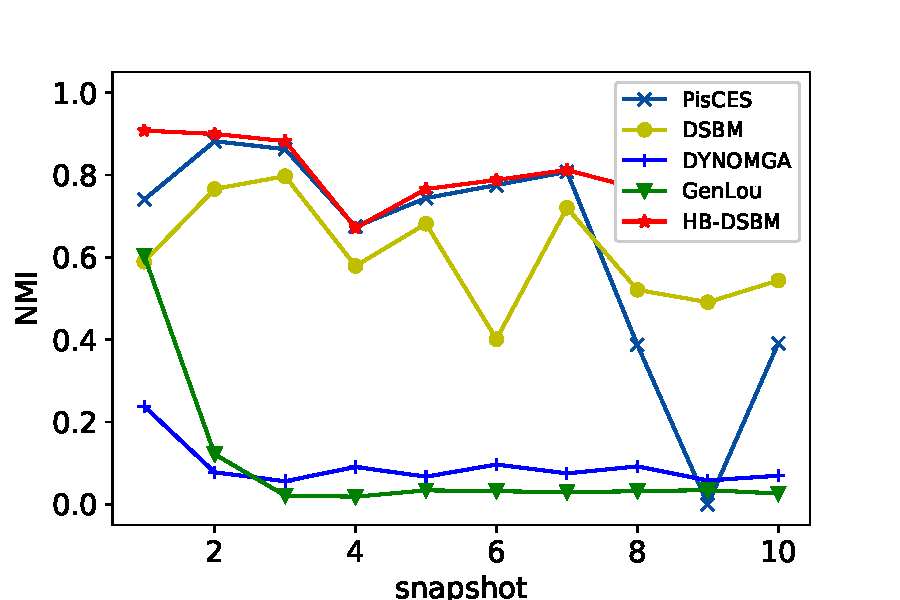
\includegraphics[width=.48\textwidth]{./figure/compare5320.pdf}
	}
	\subfigure[$\sigma=5,nC=9,aD=20$]{
		% \label{Fig.vis.1}
		\label{Fig.4.2.d}
		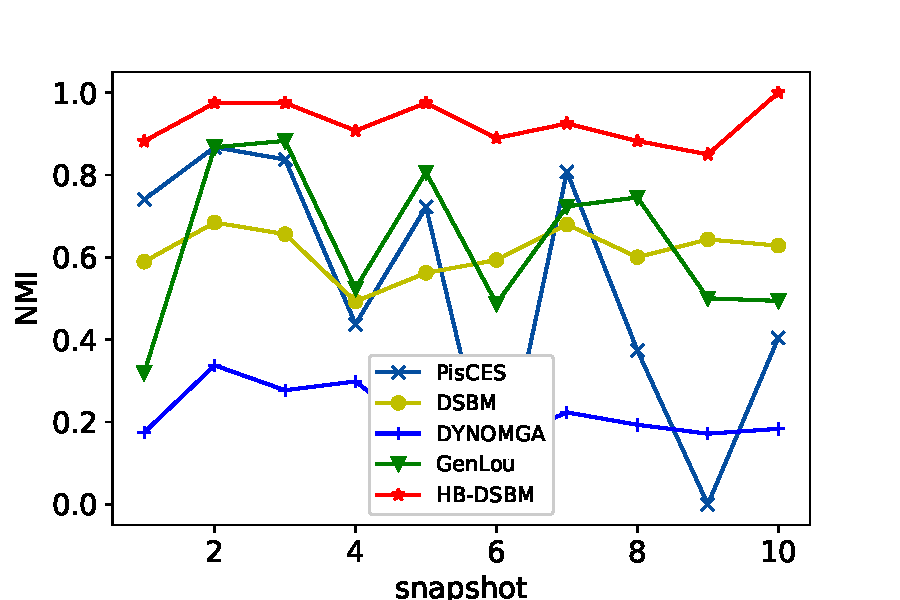
\includegraphics[width=.48\textwidth]{./figure/compare5920.pdf}
	}
	\caption{$data1$四种不同参数设置的不同方法NMI对比。}
	\label{fig.4.2}
\end{figure}

至于$data2$,NMI的结果显示如图~\ref{fig.4.3}所示,HB-DSBM依然具有最好的效果。在该数据集中,PisCES显示出比除HB-DSBM外其他方法更好的效果,而DSBM却显示除了最差的NMI表现,因为其利用吉布斯采样对模型进行求解,使得该模型在大规模数据中的有限次迭代中很难达到局部最优,即使是在每个网络快照$1000$个节点的数据集中。



\begin{figure}[htbp]
	\centering
	\subfigure[扩展事件网络]{
		% \label{Fig.vis.1}
		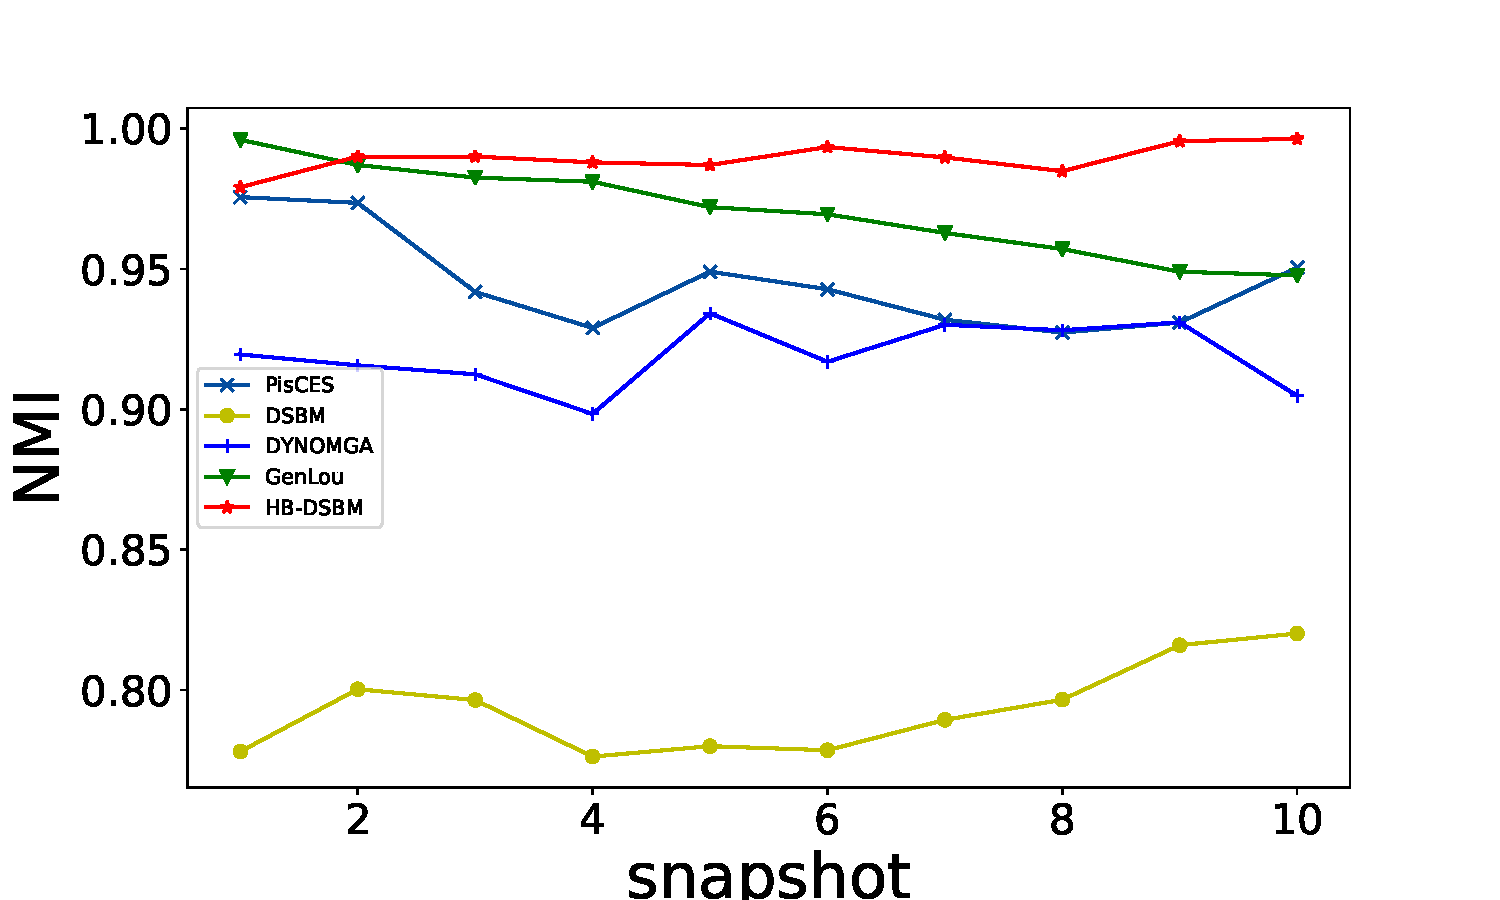
\includegraphics[width=.48\textwidth]{./figure/asonexp11.pdf}}
	\subfigure[社团交换事件网络]{
		% \label{Fig.vis.1}
		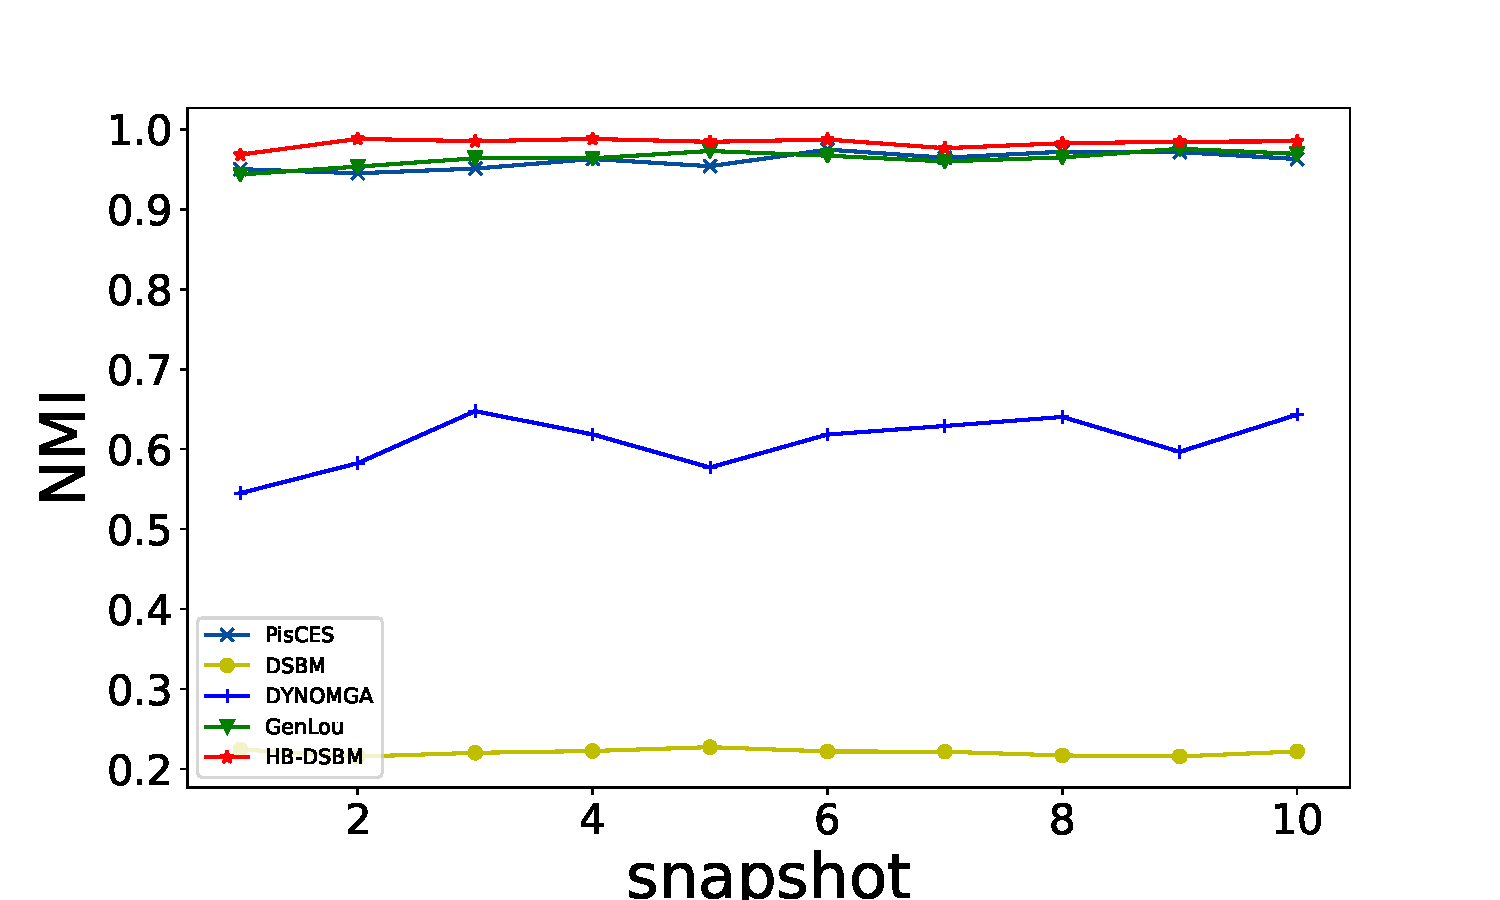
\includegraphics[width=.48\textwidth]{./figure/swi1.pdf}
	}
	\caption{$data2$两个事件网络的不同方法NMI对比。}
	\label{fig.4.3}
\end{figure}

真实世界数据集的实验如图~\ref{fig.4.4}~图\ref{fig.4.5}(a)所示,分别为KIT-email数据及DBLP数据。如图~\ref{fig.4.4}所示,HB-DSBM在KIT-email数据集中的NMI表现均高于其余方法,证明HB-DSBM不仅在生成数据集中具有较好表现,在真实世界数据集中也具有很好的社团检测效果。这里要强调的一点是,HB-DSBM在$t=1$的时候,效果并不比其余方法具有明显提升,因为HB-DSBM的改进主要注重在动态社团检测中节点的多层次演化,因此在第一个网络快照中的效果并不明显,而随着$t$的增长,HB-DSBM的效果会越来越好。




\begin{figure}[htbp]
	\centering
	\subfigure[以两个月为间隔划分快照的网络]{
		% \label{Fig.vis.1}
		\label{fig.4.4.a}
		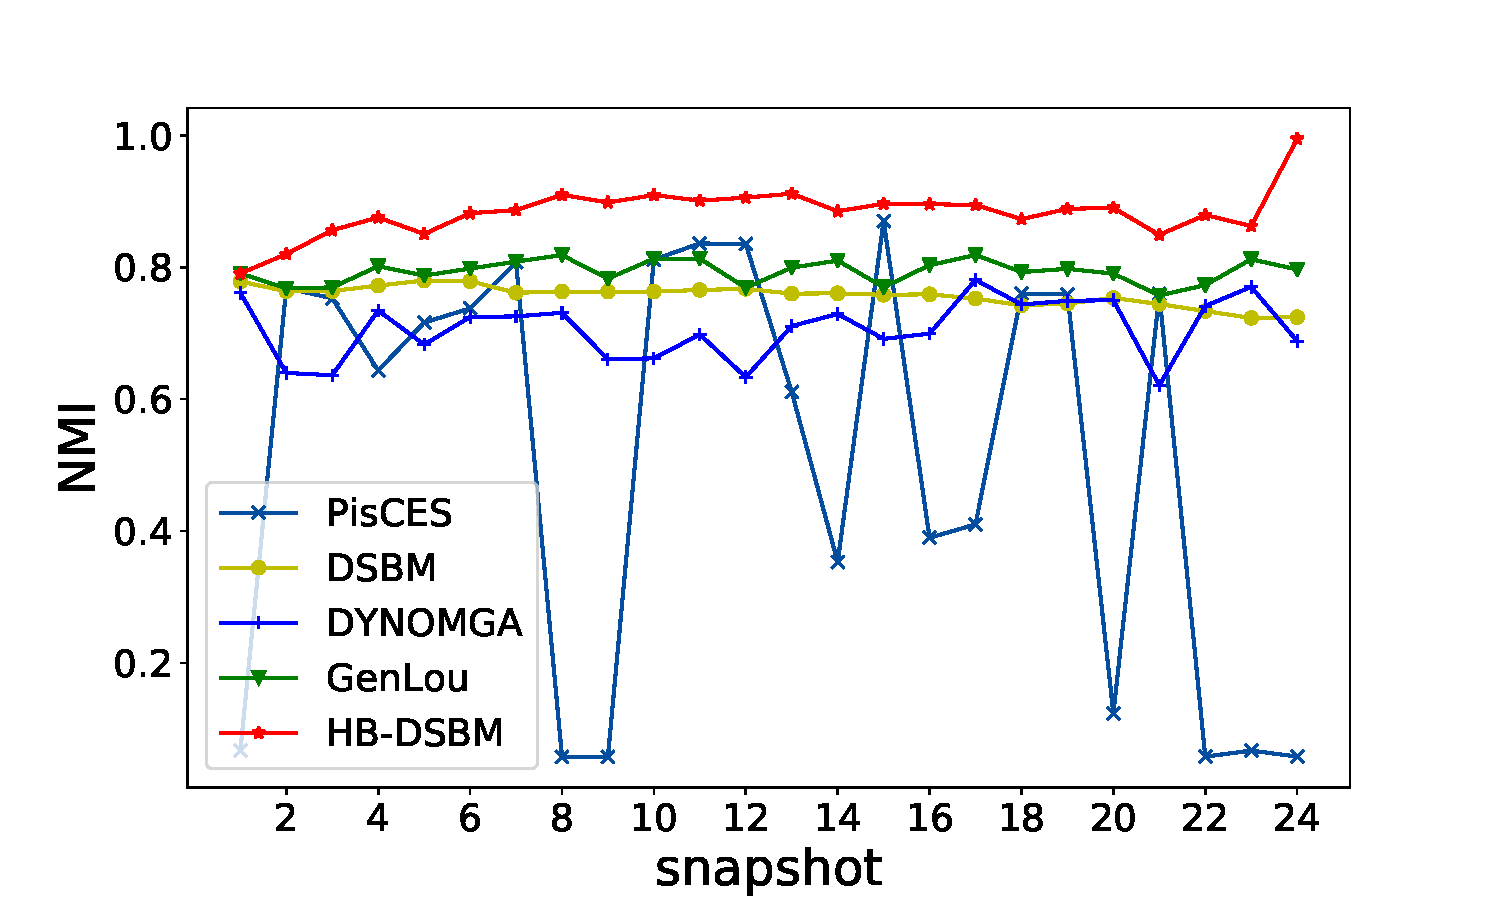
\includegraphics[width=.48\textwidth]{./figure/compareInter2t.pdf}
	}
	\subfigure[以三个月为间隔划分快照的网络]{
		% \label{Fig.vis.1}
		\label{fig.4.4.b}
		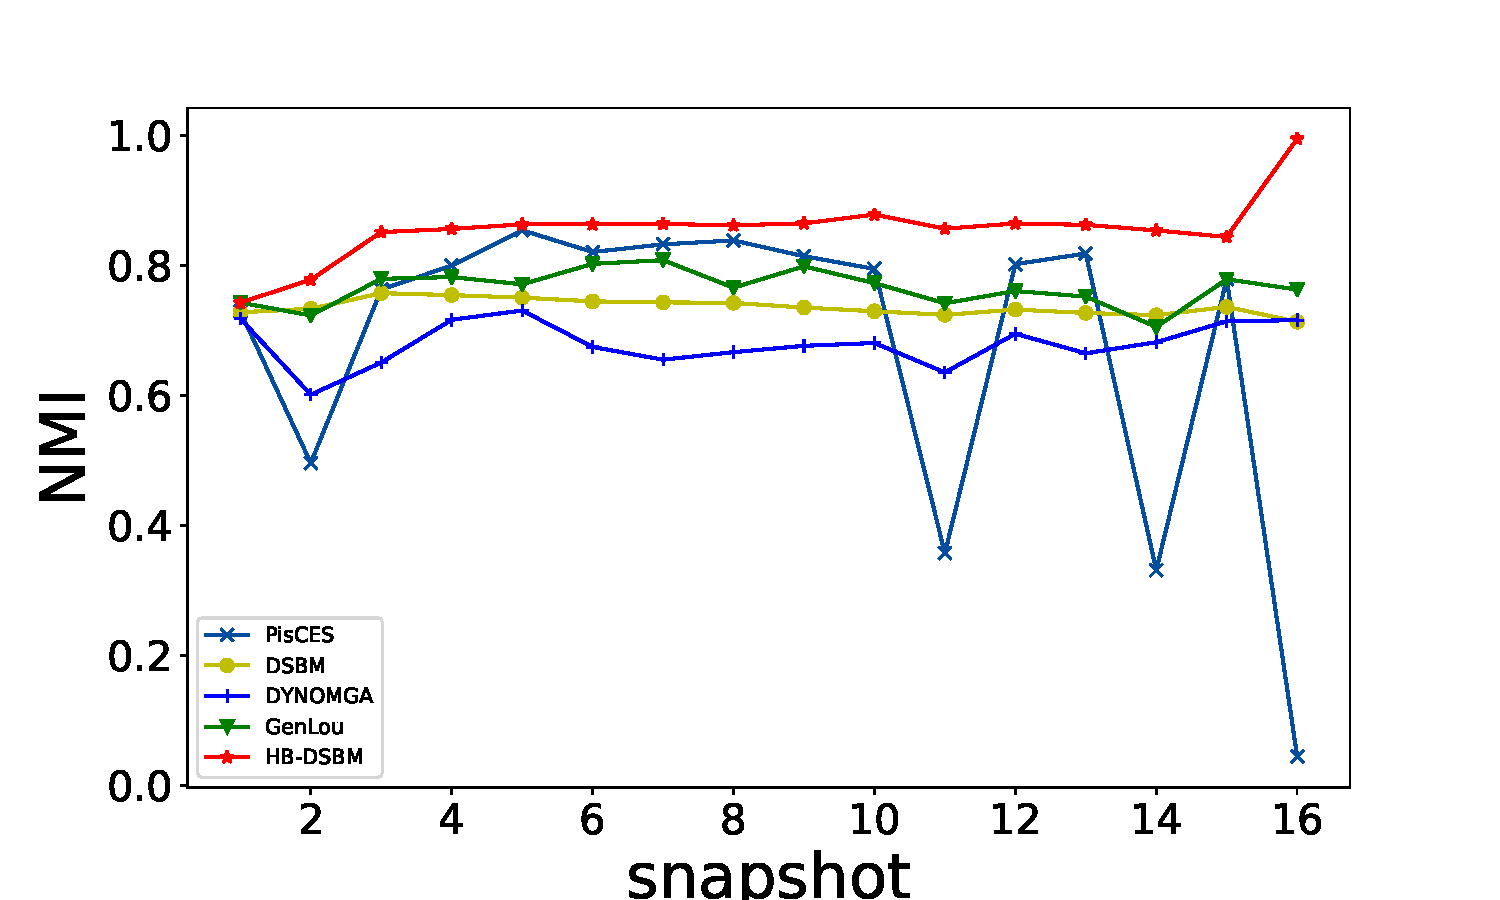
\includegraphics[width=.48\textwidth]{./figure/compareInter3.pdf}
	}
	\caption{KIT-email数据不同时间间隔划分的切片网络的不同方法NMI对比}
	\label{fig.4.4}
\end{figure}


而DBLP数据的同类方法对比如图\ref{fig.4.5}(a)所示,HB-DSBM的效果明显高于其他方法,再次证明了本模型的有效性。而DSBM的效果也优于其他方法,因为DSBM为生成模型,其同时融合了不同网络快照的社团检测与社团演化。而PisCES的噪声敏感性使得其在DBLP数据中的表现非常差,将所有节点划分到了同一个社团中。该数据集的不同方法NMI对比也再次证明了本文提出的动态网络社团演化层次贝叶斯结构的有效性。

\begin{figure}[htbp]
	\centering
	\subfigure[DBLP数据的NMI对比]{
		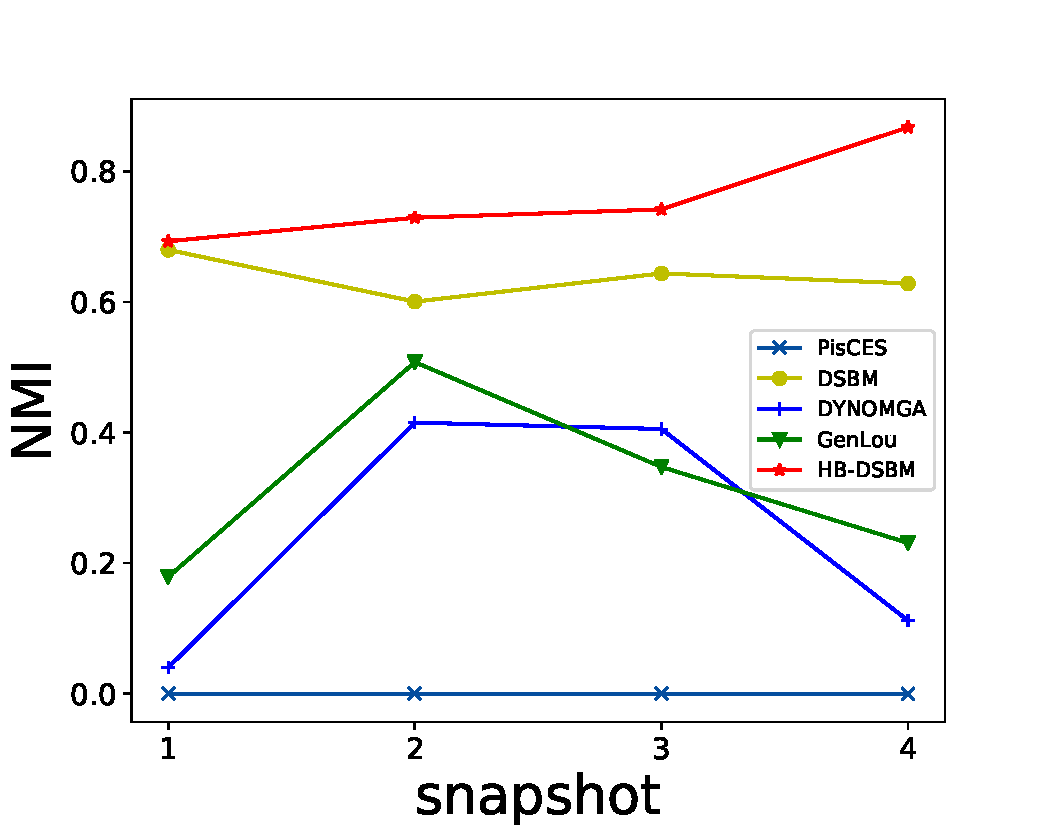
\includegraphics[width=.48\textwidth]{./figure/dblp_t6789.pdf}
		\label{Fig.4.5.a}
	}
	\subfigure[DBLP以及$data1$的社团转移矩阵可视化]{
		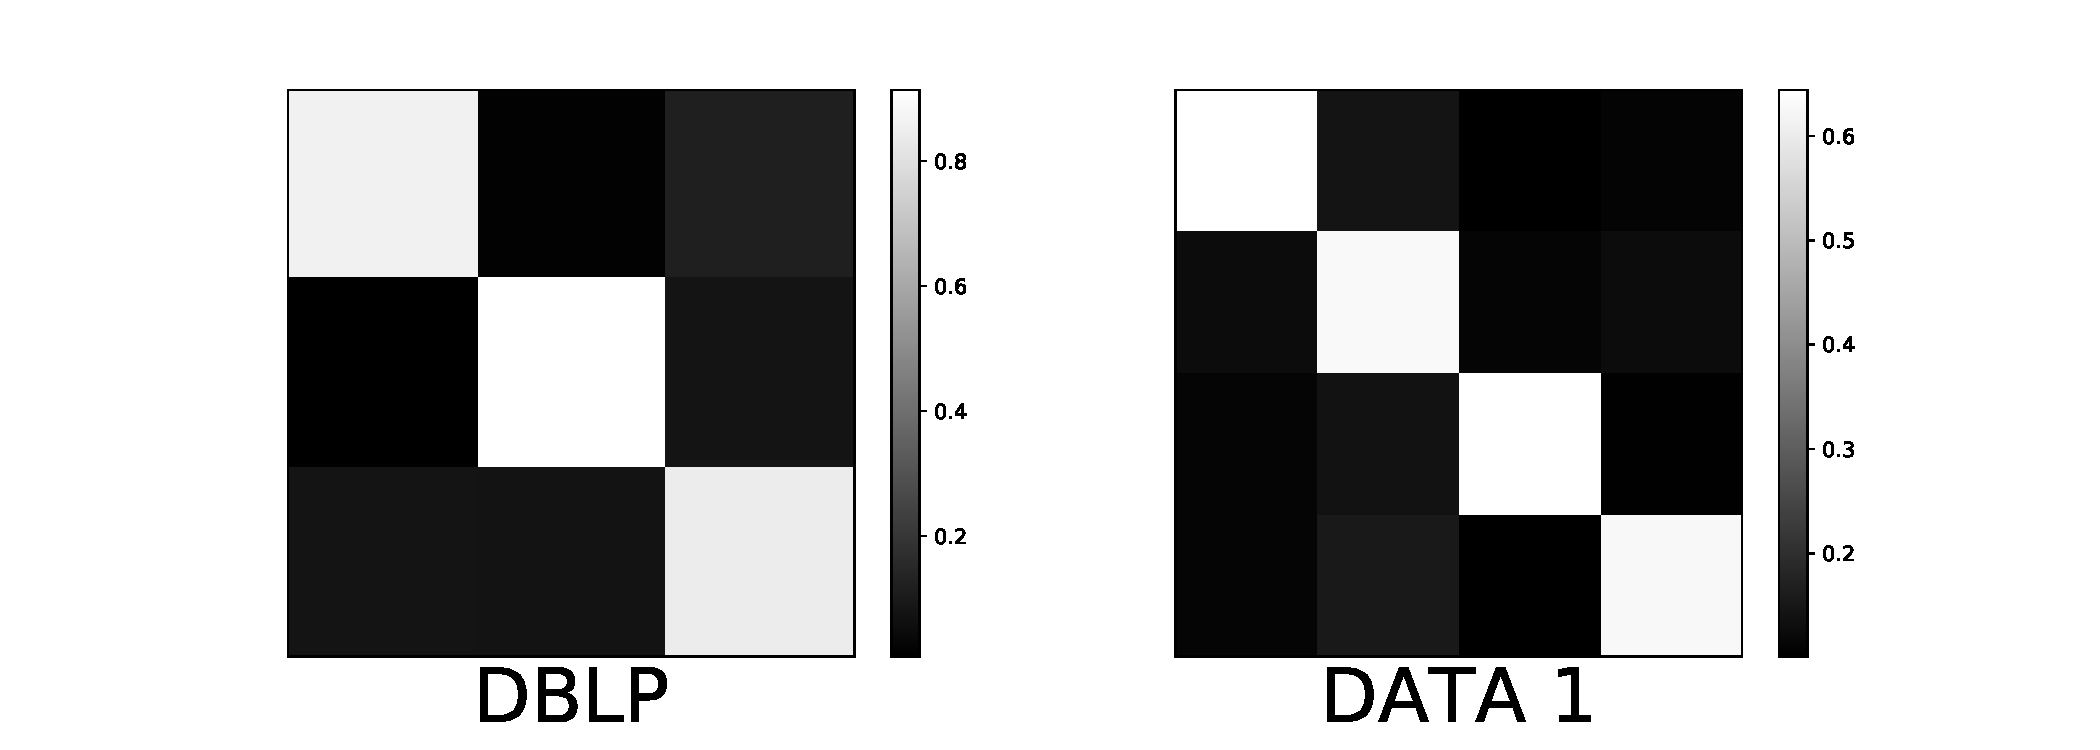
\includegraphics[width=.48\textwidth]{./figure/communityHeatMap.pdf}
		\label{Fig.4.5.b}
	}
	\caption{DBLP数据社团检测及演化效果图。}
	\label{fig.4.5}
\end{figure}


\subsection{社团演化分析}

以往的模型如DSBM将在同一个社团的节点视作等价,也就是说在同一个社团的两个节点在模型中没有任何差别,它们具有相同的社团转移倾向,并且DSBM中的社团转移倾向矩阵并不会随着时间推移而变化。也就是说,以往的模型只考虑了节点的社团级别的演化倾向,并且是不变的。在HB-DSBM中,隐变量$C$和$A$分别代表了节点级别和社团级别的演化倾向,同时通过层次生成结构将这两个参数整合到了一起。模型社团级别的转移倾向矩阵$A$的可视化如图\ref{fig.4.5}(b)所示,图中分别展示了DBLP和$data1$的社团级别的转移倾向。然而社团级别的转移倾向并不是一成不变的,社团级别的转移倾向会随着时间变化,如图\ref{fig.4.6}可以看到,HB-DSBM准确把握住了不同网络快照中的社团级别的节点社团转移倾向。

\begin{figure}[htbp]
	\centering
	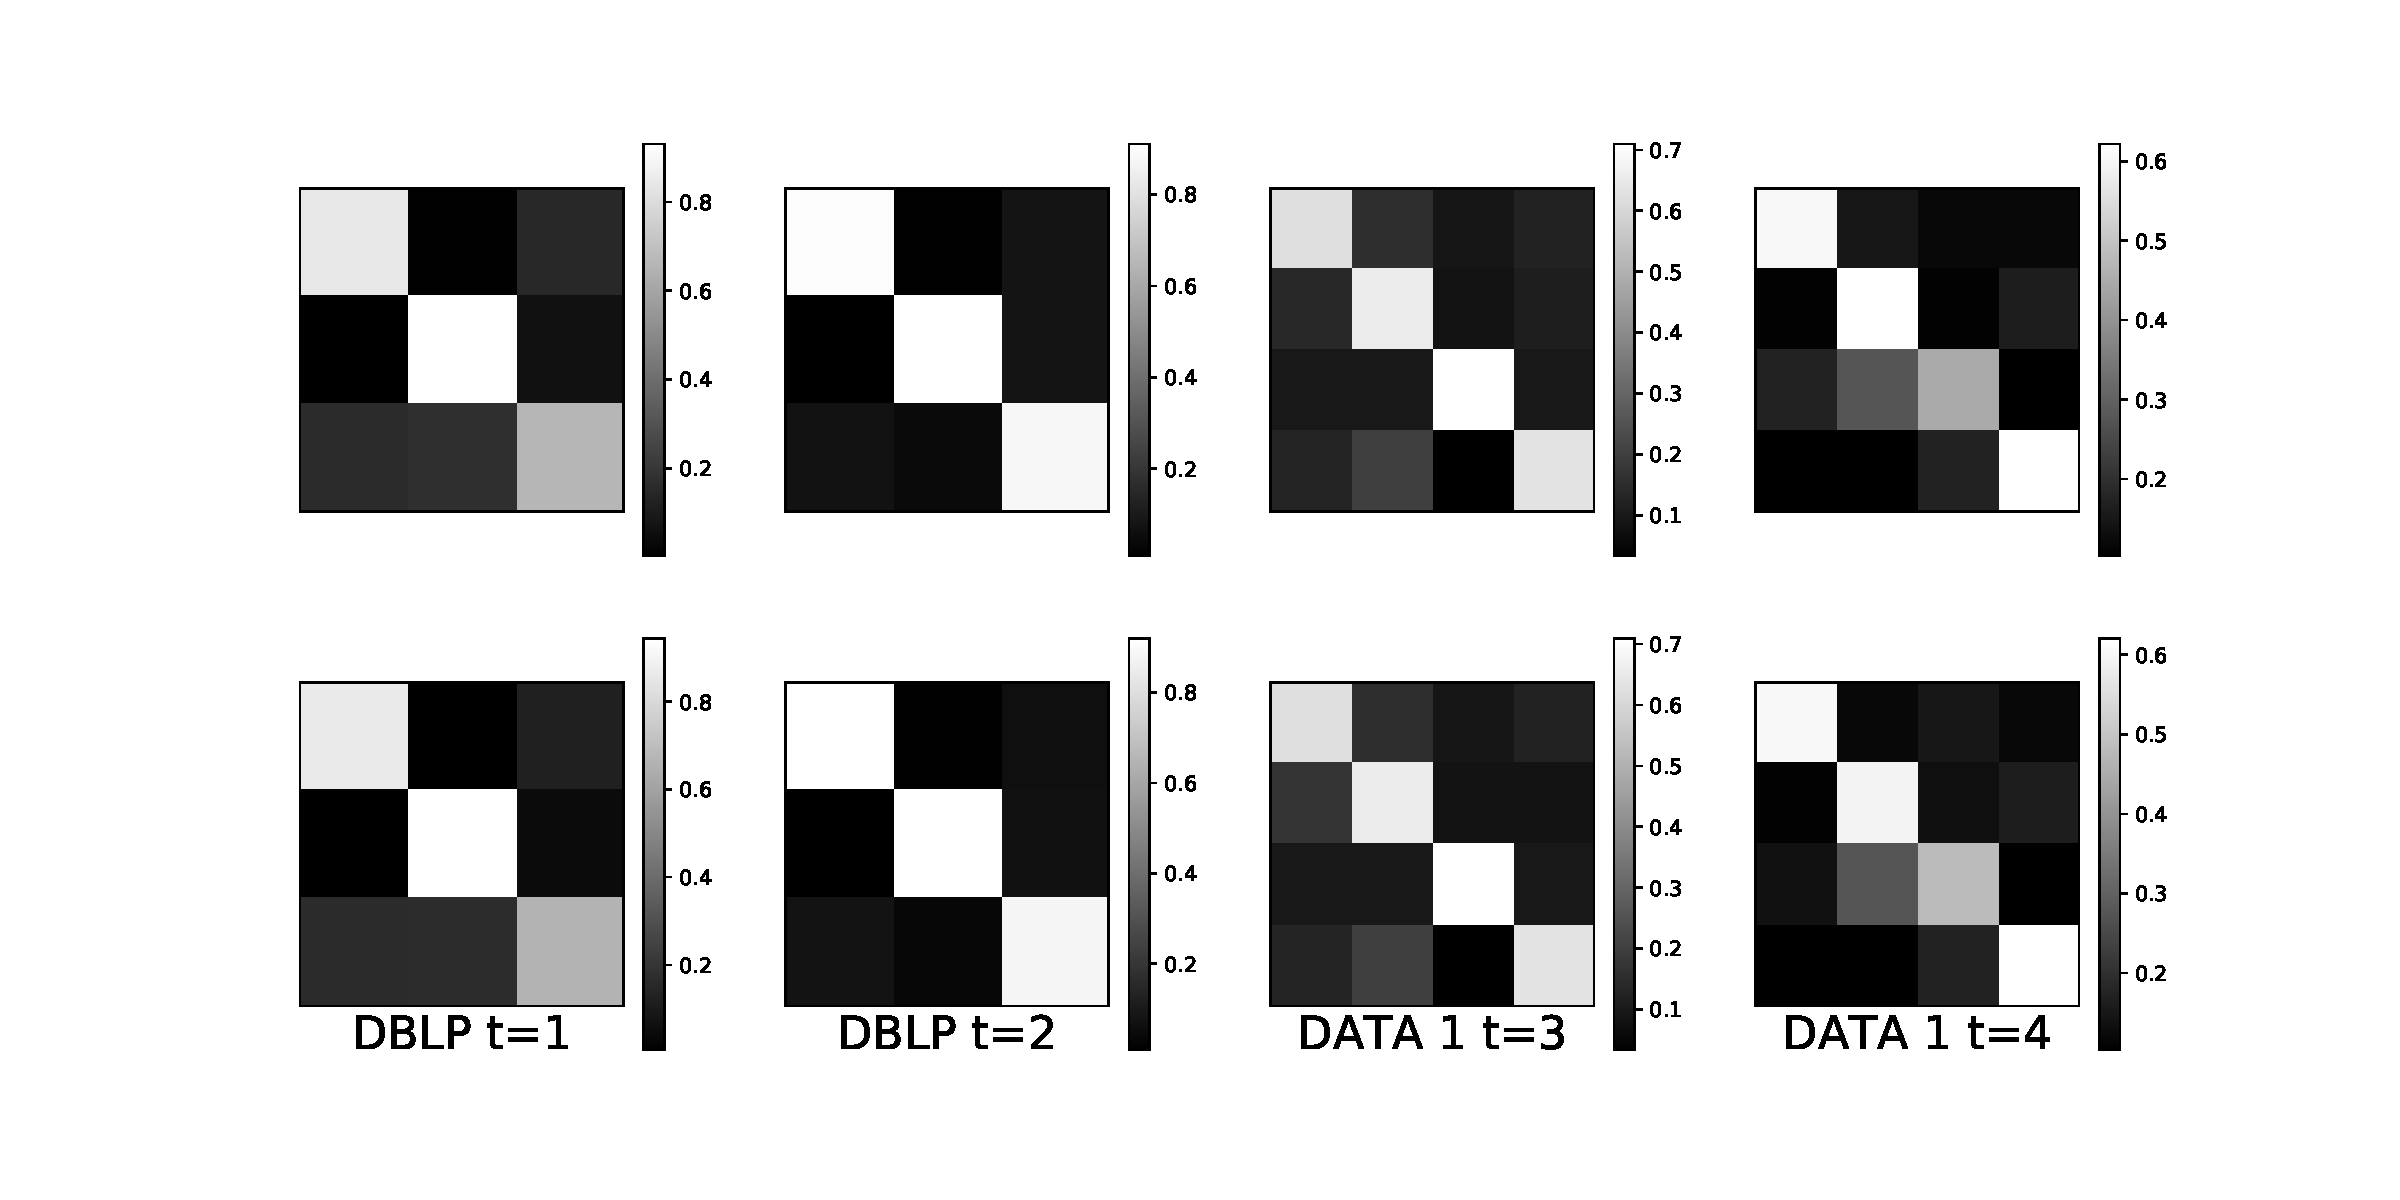
\includegraphics[width=.8\textwidth]{./figure/communityHeatMapt.pdf}
	\caption{基于HB-DSBM模型的社团级别转移矩阵$A$分别在DBLP和$data1$数据的可视化(上半部分)与真实社团转移真相的可视化(下半部分)之间的对比。}
	\label{fig.4.6}
\end{figure}


而同一社团的节点也具有不同的社团转移倾向,图\ref{fig.4.7}展示了DBLP数据中不同研究领域的作者的研究兴趣领域发生转移的倾向的异质性。例如,$Theo Gevers$在$2009$年发表了一篇数据挖掘的论文。根据模型的节点转移矩阵的计算,他有很大的倾向继续在数据挖掘领域发表论文,而事实也验证了模型的推算。
\begin{figure*}[htbp]
	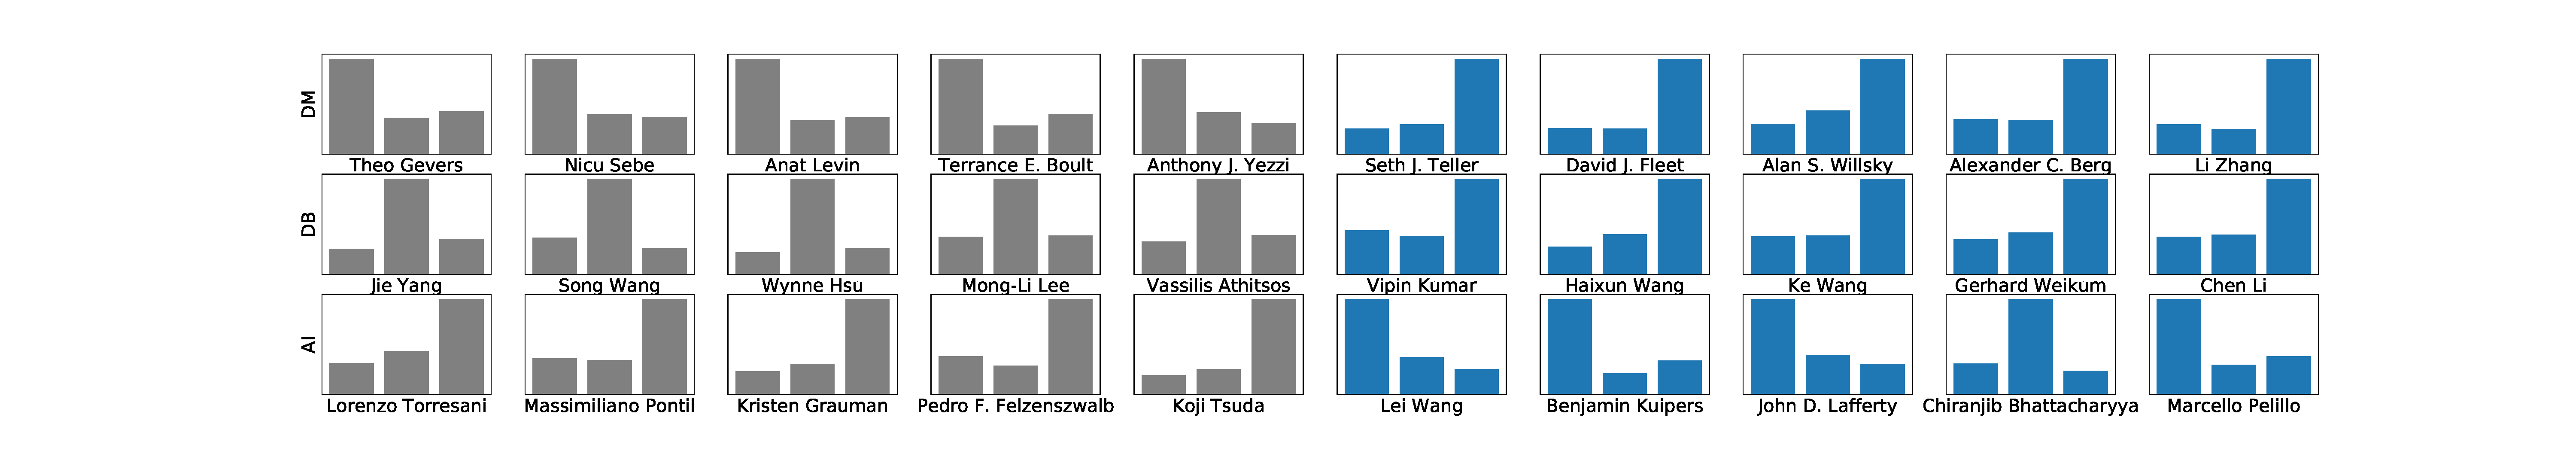
\includegraphics[width=\textwidth]{./figure/nodes_compare.pdf}
	\caption{DBLP数据集中部分节点($2009-2010$年)的社团转移倾向可视化(基于节点级别转移倾向参数$C$)。每个柱状图代表一个节点的转移倾向,从左到右分别为DM,DB,AI。所有柱状图共三行,每行代表一个领域,从上到下分别为DM,DB,AI。灰色的柱状图代表节点社团转移倾向与其所在社团转移倾向一致,而蓝色的柱状图代表节点的转移倾向与其所在社团的转移倾向不一致。}
	\label{fig.4.7}
\end{figure*}

通过HB-DSBM对DBLP数据的分析,本文还发现了一个有趣的现象,即大部分作者都倾向于在几年之内转换他们的研究兴趣领域。换句话说,只有很少一部分的作者会长期停留在同一个研究领域。如图\ref{fig.4.8}所示,$Svetlana Lazebnik$倾向于每两年转换一次研究兴趣领域,而这个时间间隔对$Jing Peng$来说则为三年。同时$Andrew W. Fitzgibbon$从数据挖掘在$t=7$时将研究领域转移到了人工智能领域。$Amnon Shashua$则将研究兴趣领域从人工智能转移到数据挖掘进行研究,四年后又将研究兴趣领域转移回了人工智能。

 \begin{figure}[htbp]
 	\centering
	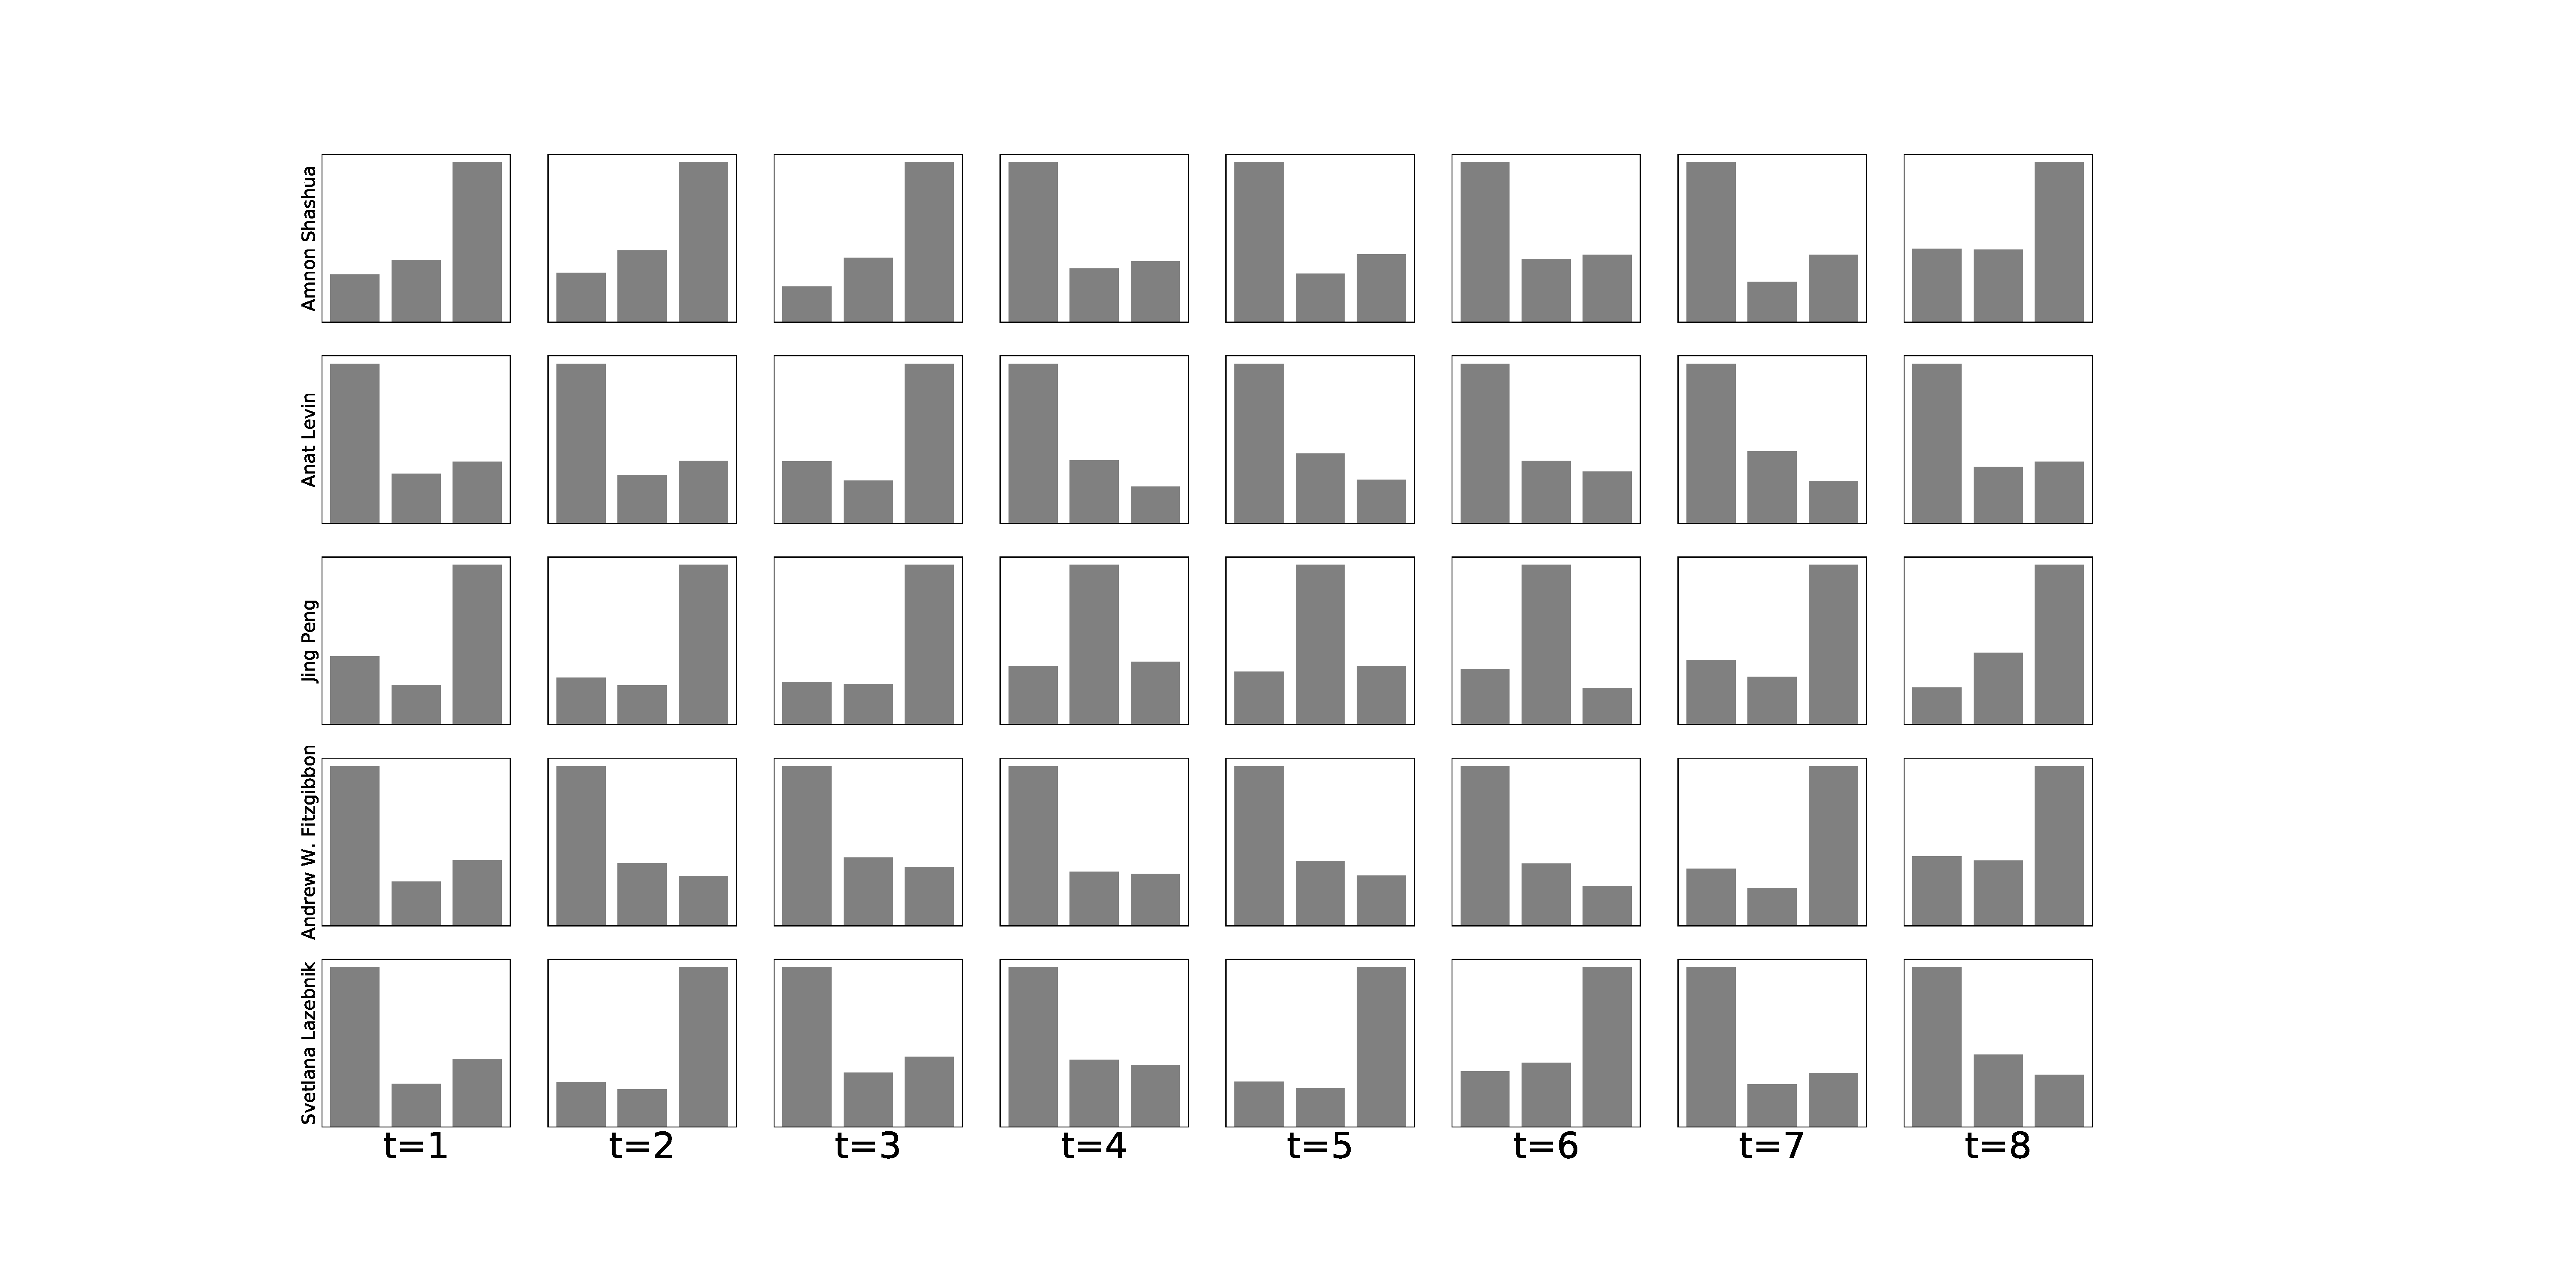
\includegraphics[width=.9\textwidth]{./figure/nodes_evoluton1.pdf}
	\caption{DBLP数据选取的五个作者($Amnon Shashua, Anat Levin, Jing Peng, Andrew  W. Fitzgibbon, Svetlana Lazebnik$)的$8$年的转移倾向可视化。每个柱状图代表作者的社团转移倾向矩阵,从左到右分别为DM,DB,AI。}
	\label{fig.4.8}
\end{figure}

\section{本章小结}
本章介绍了层次贝叶斯动态随机块模型,其层次贝叶斯生成结构能够同时融合节点级别以及社团级别的社团演化模式。同时本文利用变分推断对模型参数进行估计,利用合理的优化策略,模型可以适应大规模数据的计算。同类方法的对比也显示出HB-DSBM在动态网络社团检测任务中更加高效准确。在第五章将会介绍基于手机信令数据结合HB-DSBM的城市风险计算案例分析,以此来验证复杂网络算法在城市风险计算中的重要作用。
\clearpage{\pagestyle{empty}\cleardoublepage}
% !Mode:: "TeX:UTF-8"

%\chapter{城市风险计算案例分析}
%\section{数据集介绍}
%
%\section{小结}

\clearpage{\pagestyle{empty}\cleardoublepage}
% !Mode:: "TeX:UTF-8"

\markboth{总结与展望}{总结与展望}
%\addcontentsline{toc}{chapter}{结\quad 论} %添加到目录中
\chapter{总结与展望}

本文关注于动态复杂网络社团检测问题,依托于随机块模型框架,从模型的角度研究动态网络中的社团演化问题,同时探究了影响动态网络中节点社团转移的结构属性。随后从城市风险计算的角度对本文的方法以及探究的规律的有效性进行了实证分析。本章对本文的研究内容和研究成果进行总结分析,并指出其中模型的不足之处与未来的研究思路。
\section{总结}
社团结构作为复杂网络的重要任务之一,对于理解复杂网络结构形成、功能探索和领域应用如风险计算有重要的作用。而复杂网络的动态演化给社团检测带来了新的挑战,包括社团结构的演化、社团的产生与消亡、社团的分裂与合并等问题,与此同时,动态网络的社团检测也迫切需要我们对社团的演化行为进行建模。作为复杂网络社团检测的重要方法之一,随机块模型对网络的生成机制解释性的非常好,可以有效地建模复杂网络中社团的形成机制。而基于随机块模型构建的动态网络模型能够在有效地建模网络形成机制的同时把握网络中的社团演化机制。本文立足于动态随机块模型框架,从模型的角度对动态网络的社团结构进行建模,旨在解决动态网络中节点社团演化机制的问题。于此同时,本文还对节点的结构属性与节点的社团归属演变之间的关系通过多个真实数据集进行了探究,得到了对社团演化机制探究至关重要的结论。在应用方面,本文利用手机信令数据验证了本文提出的模型对城市风险计算的有效性。本文的主要工作和贡献点总结如下:
\begin{itemize}
	\item 本文利用15个真实复杂网络数据集,包括社交网络数据(如twetter、facebook等)、wiki数据及社区通话数据等,通过TILES方法对数据进行动态网络社团检测,同时利用决策树将相邻时间片的节点是否发生社团转移作为二分类标签,将节点的结构属性通过特征工程组合为决策树的分类特征对节点进行二分类。通过对决策树分类后的分类模型中的特征重要性进行计算,本文得出结论:节点的度和节点的平均邻居度对节点的社团归属变化影响最大。并且在后续的案例分析中,本文找到了与之相佐证的真实情景。
	\item 基于动态随机块模型(DSBM),本文提出了层次贝叶斯动态随机块模型(HB--DSBM)。该模型在相邻时间片引入了节点级别的社团转移参数,并提出了层次贝叶斯结构来生成社团级别的节点社团转移参数和节点级别的社团转移参数,并利用更细粒度的节点级别社团转移参数生成节点的在动态网络的社团归属。同时本文还对HB-DSBM提出了高效的变分推断算法,通过变分推断算法来对模型近似求解,同时提升了其算法运行效率,比之传统的DSBM模型运行效率更能适应大规模数据。通过将HB-DSBM和不同类的动态社团检测方法进行对比,并进行了社团演化分析对比,结果显示HB-DSBM在动态社团检测效果高于同类方法的同时,受益于更细粒度的社团转移参数,对于动态网络的社团演化分析更加精准。
	\item 通过对手机信令数据的处理,结合天津地块信息构建了多层复杂网络,并利用HB-DSBM对手机信令数据进行社团划分,并进一步通过社团标签-事件的提取方法计算出事件以及事件发生地以及事件发生时间。随后根据相关文献,通过合理的设计打分策略评判出每个事件的风险程度,并结合实际评判其合理性,以证明文章提出的HB-DSBM在风险计算中的可行性以及有效性。
\end{itemize}

\section{展望}
本文对于节点结构特征对社团演化的影响的探究以及构建的HB-DSBM模型对动态复杂网络社团演化的探究具有一定的贡献,但是随着最新的动态网络社团检测建模发展趋势以及城市风险计算发展的影响,本文的许多工作需要我们进行改进或者进一步研究。同时针对城市风险计算的需求,本文利用HB-DSBM对天津市手机信令数据进行社团检测,并利用相关文献进行事件提取以及每个事件的风险值评估,得到了风险事件的结果,然而该实证的计算依然存在一些待完善的部分。具体如下:
\begin{itemize}
	
	\item 对于节点结构特征对社团演化的影响的探究中,我们得出结论:节点的度和节点的平均邻居度对节点的社团关系变化影响至关重要。其中,节点的度对节点的社团关系变化的影响是显而易见的,同时目前也有很多方法将节点的度应用于社团检测中来增强社团检测的效果,这些方法也都取得了预期的结果,这侧面证明了节点的度在动态网络社团检测中的重要作用。然而,节点的平均邻居度对节点社团转移的影响的内在规律还需要我们进一步探究,相信在不就的将来,节点的平均邻居度也可以有效的作用于动态网络社团检测。
	\item HB-DSBM模型在融合了节点粒度的转移参数后,确实对动态网络社团检测以及社团演化分析都起到了很大的作用,但是该模型在引入了如此细粒度的参数后,使得其参数空间变得非常大,虽然本文提出了变分推断以及在实现中使用了随机采样等策略一定程度上降低了算法的复杂度,但是仍然达不到真正应用于生产的程度。因此对模型适当改进以降低其参数规模是HB-DSBM的下一步改进方向。
	\item HB-DSBM模型改进自DSBM,这使得其继承了DSBM的一大缺陷,即该模型不能适用于重叠社团的检测。在现实世界大部分情景中,同一个节点可以属于多个社团,例如大学学生可以加入多个兴趣社团等。该问题在静态网络随机块模型中得到了较好的解决,即混合随机块模型。而针对动态随机块模型的重叠社团问题,也已经有一些方法,但是均存在一些缺陷,因此对HB-DSBM进行适当改进使得其能够检测重叠社团也是其下一步重要的改进方向之一。
	\item HB-DSBM模型的一大假设就是需要预先知道动态网络中社团的个数,这在真实数据中是不可行的,例如在社交网络中,兴趣小组的个数不可能在不经聚类之前就提前知晓。同类方法的处理方式一般为在计算时设置社团个数$K=\log N$,其中,$N$为网络中的节点个数。再通过适当的方法将没有实际意义的社团舍弃以达到模型选择的目的(例如仅有一个节点的社团),而此种方法会大大增加算法的计算量,因此也不是很好的模型选择方法。HB-DSBM继承自DSBM,因此该方法的模型选择可以参考现有的针对DSBM的模型选择方法进行改进,如利用狄利克雷过程利用数据自动确定社团个数等。因此通过对HB-DSBM进行适当的改进来使该模型能够根据数据特征自动确定社团个数,即模型选择,也是其下一步改进的方向之一。
	\item 本文在实证部分,仅融合了手机信令数据与天津市地块数据构建了二层复杂网络对事件进行提取并对每个事件进行了风险分析。而真正的城市风险计算需要融合地块、事件、人员、人员行为等包括物理空间和网络空间的数据进行多层次融合以及计算之后才能得出准确的风险计算结果,多源信息融合也是风险计算中进行风险预测、风险决策、风险管控的基础,因此对于风险计算部分,下一步需要改进的就是完善数据收集以及信息融合的底层架构,这样才能在未来进行更深层次的风险计算。
\end{itemize}

\clearpage{\pagestyle{empty}\cleardoublepage}
%%%%%%%%%% 正文部分内容  %%%%%%%%%%

%%%%%%%%%%  参考文献  %%%%%%%%%%
\defaultfont
\bibliographystyle{TJUThesis}
\phantomsection
\markboth{参考文献}{参考文献}
\addcontentsline{toc}{chapter}{参考文献}          % 参考文献加入到中文目录
%\nocite{*}                                        % 若将此命令屏蔽掉,则未引用的文献不会出现在文后的参考文献中。
\bibliography{references/reference}
\clearpage{\pagestyle{empty}\cleardoublepage}
% !Mode:: "TeX:UTF-8"

\markboth{发表论文和参加科研情况说明}{发表论文和参加科研情况说明}
\addcontentsline{toc}{chapter}{发表论文和参加科研情况说明}
\chapter*{发表论文和参加科研情况说明}
\setlength{\parindent}{0em}
\textbf{(一)发表的学术论文}
\vspace*{1em}
\textbf{(二)参与的科研项目}
\vfill
\hangafter=1\hangindent=2em\noindent

\setlength{\parindent}{2em}
                   % 发表论文和参加科研情况说明
\clearpage{\pagestyle{empty}\cleardoublepage}
% !Mode:: "TeX:UTF-8"

\markboth{致\quad 谢}{致\quad 谢}
\addcontentsline{toc}{chapter}{致\quad 谢} %添加到目录中
\chapter*{致\quad 谢}









               % 致谢
\clearpage
\end{CJK*}                                        % 结束中文字体使用
\end{document}                                    % 结束全文
